% CS701 team report. CVPR style (template taken from the team's draft on origin/jinling); the complete experiment log follows as an appendix.
% Build: tectonic main.tex   (tables/ and figures/ are written by gen_report.py)
\documentclass[10pt,twocolumn,letterpaper]{article}
\usepackage[T1]{fontenc}
\usepackage[pagenumbers]{cvpr}
\usepackage{times}
\usepackage{graphicx}
\usepackage{amsmath,amssymb}
\usepackage{booktabs}
\usepackage{enumitem}
\usepackage{xcolor}
\usepackage{microtype}
\definecolor{cvprblue}{rgb}{0.21,0.49,0.74}
\usepackage[breaklinks,colorlinks,allcolors=cvprblue]{hyperref}
\def\paperID{Team 7}
\def\confName{CS701}
\def\confYear{2026}
\newcommand{\dm}{\ensuremath{\Delta m}}
\usepackage{longtable}
\usepackage{array}
\newcommand{\TEAMMATES}{\textcolor{red}{[other authors: TBD]}}
\newcommand{\PTWO}{61.25}
\newcommand{\GPUH}{\textcolor{red}{TBD}}


% Flags and file paths in \texttt, with line breaks allowed at space _ / , ; . = : and inside words after a single
% hyphen, never inside the leading -- of a flag. The argument is detokenized, so no escaping is needed inside.
\newcommand{\flsize}{\fontsize{9}{11}\selectfont}
\ExplSyntaxOn
\tl_new:N \l__fl_p_tl
\tl_new:N \l__fl_pp_tl
\cs_new_protected:Npn \__fl_char:n #1
  {
    \bool_lazy_all:nT
      {
        { \str_if_eq_p:Vn \l__fl_p_tl { - } }
        { ! \str_if_eq_p:nn { #1 } { - } }
        { ! \str_if_eq_p:Vn \l__fl_pp_tl { - } }
        { ! \str_if_eq_p:Vn \l__fl_pp_tl { ~ } }
        { ! \tl_if_empty_p:N \l__fl_pp_tl }
      }
      { \penalty 50 \hskip 0pt \relax }
    \str_case:nnF { #1 }
      {
        { ~ } { \hskip 0.6em plus 0.4em minus 0.1em \relax }
        { _ } { #1 \penalty 50 \hskip 0pt \relax }
        { / } { #1 \penalty 50 \hskip 0pt \relax }
        { , } { #1 \penalty 50 \hskip 0pt \relax }
        { ; } { #1 \penalty 50 \hskip 0pt \relax }
        { . } { #1 \penalty 200 \hskip 0pt \relax }
        { = } { #1 \penalty 200 \hskip 0pt \relax }
        { : } { #1 \penalty 200 \hskip 0pt \relax }
      }
      { #1 }
    \tl_set_eq:NN \l__fl_pp_tl \l__fl_p_tl
    \tl_set:Nn \l__fl_p_tl { #1 }
  }
\NewDocumentCommand \fl { m }
  {
    \texttt
      {
        \flsize \hyphenchar \font = -1 \relax
        \tl_clear:N \l__fl_p_tl
        \tl_clear:N \l__fl_pp_tl
        \str_map_inline:nn { #1 } { \__fl_char:n { ##1 } }
      }
  }
\ExplSyntaxOff
\newcommand{\mn}{\ensuremath{-}}
\newcommand{\x}{\ensuremath{\times}}
\newcommand{\pmm}{\ensuremath{\pm}}
\newcommand{\ap}{\ensuremath{\approx}}
\renewcommand{\to}{\ensuremath{\rightarrow}}
\newcommand{\sg}{\ensuremath{\sigma}}
\newcommand{\lam}{\ensuremath{\lambda}}
\newcommand{\sn}{\textsuperscript{$\dagger$}}
\newcommand{\dc}{\textsuperscript{$\ddagger$}}
\newcommand{\vtp}{v3\ensuremath{'}}

% Keeps the generated tables at their place in the text (they are written as \begin{table}[t]).
\makeatletter
\newenvironment{heretable}[1][]{\par\medskip\noindent\begin{minipage}{\linewidth}\def\@captype{table}}{\end{minipage}\par\medskip}
\makeatother

\newcolumntype{L}[1]{>{\raggedright\arraybackslash\hspace{0pt}}p{#1}}
\newcolumntype{R}[1]{>{\raggedleft\arraybackslash\hspace{0pt}}p{#1}}
\setlength{\LTcapwidth}{\textwidth}
\newenvironment{lt}[1]{\footnotesize\renewcommand{\flsize}{\fontsize{7}{8.5}\selectfont}\setlength{\tabcolsep}{3pt}\setlength{\LTpre}{5pt}\setlength{\LTpost}{6pt}\begin{longtable}{@{}#1@{}}}{\end{longtable}}
\newcommand{\lthead}[2]{\toprule #2\\ \midrule \endfirsthead \multicolumn{#1}{@{}l}{\emph{(continued)}}\\ \toprule #2\\ \midrule \endhead \bottomrule \endlastfoot}
\setlength{\parskip}{3pt plus 1pt}
\setlength{\parindent}{0pt}
\emergencystretch=3em
\setcounter{tocdepth}{1}



\title{One Frozen DINOv3, Wide LoRA and a Tiny-Object Cascade:\\Multi-Task Learning on SAR Images under a 40\,M Budget}
\author{CS701 Team 7 (\texttt{cs701-team07})\\
Junkai Chen, \TEAMMATES\\
Singapore Management University}

\begin{document}
\maketitle

\begin{abstract}
One model must classify a SAR image into nine scene classes and detect its objects, half of which are smaller than a $16{\times}16$ ViT patch, under limits of 130\,M total and 40\,M trainable parameters. Our model keeps a DINOv3 ViT-B/16 frozen and spends the budget on LoRA rank 80 and a three-stage Cascade R-CNN built for tiny boxes. It reached $\dm=56.49$ on the Phase 1 validation board (macro-F1 95.27, mAP 55.10). The final Phase 2 entry uses the same weights plus two local-only post-processing additions. Almost all the gain over the reference comes from detection. We report what each part adds: leave-one-out ablations on a held-out split over several seeds, which we ran specifically for this report, and a post-processing ablation on full-length runs (seed 0 finished; further seeds TBD). We also report what failed, including results that won on a local split and vanished on the board.
\end{abstract}

\section{Introduction}
\label{sec:intro}
Each image has one class label and one or more boxes of that class. Teams are ranked by $\dm = 50\,[(F_1-F_1^{\text{ref}})/F_1^{\text{ref}} + (\text{mAP}-\text{mAP}^{\text{ref}})/\text{mAP}^{\text{ref}}]$, with reference scores 93.31 / 26.13 on val and 93.99 / 25.41 on test. On val, one mAP point is worth 1.91\,\dm{} and one F1 point 0.54\,\dm{}. A point of mAP therefore pays 3.6 times as much as a point of F1, so we spent nearly all our effort on detection.

Three properties of the data shaped the design. (1) Boxes are tiny: at the 512\,px input, 18.4\,\% have side ${<}8$\,px and 50.5\,\% have side ${<}16$\,px. (2) Localisation is the bottleneck, not recall alone: our final local AP falls from about 75 at IoU 0.5 to 22 at IoU 0.9. (3) Annotations carry structure a model can exploit: a sub-pixel offset and, for some class--size cells, an integer coordinate lattice (\S\ref{sec:findings}).

\section{Related work}
LoRA~\cite{hu2022lora} and MTLoRA~\cite{agiza2024mtlora} adapt frozen weights at low cost; we use a single wide LoRA. For tiny objects, NWD~\cite{wang2021nwd} replaces IoU in assignment, Cascade R-CNN~\cite{cai2018cascade} refines boxes, ViTDet~\cite{li2022vitdet} builds a pyramid from one ViT map, and ViT-Adapter~\cite{chen2023vitadapter} adds a CNN spatial prior. Soft-NMS~\cite{bodla2017softnms} and weight averaging along a trajectory~\cite{izmailov2018swa} are the two ideas behind our largest zero-cost gains. \dm{} is the usual multi-task summary~\cite{maninis2019mtl,vandenhende2021mtl}.

\section{Method}
\label{sec:method}
\begin{figure}[t]
\centering
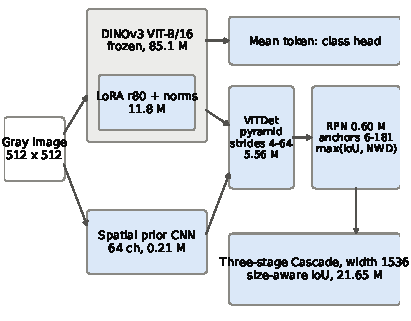
\includegraphics[width=\linewidth]{figures/model.pdf}
\caption{The final model. Only the blue blocks train (39.87\,M). Each image passes through once at $512{\times}512$.}
\label{fig:model}
\end{figure}

\textbf{Backbone.} Timm \texttt{vit\_base\_patch16\_dinov3.lvd1689m}, frozen; the RGB patch kernel is summed to one gray channel. LoRA rank 80, $\alpha{=}160$ wraps \texttt{qkv}, \texttt{proj}, \texttt{fc1} and \texttt{fc2} of all 12 blocks, and LayerNorms train.

\textbf{Neck.} A ViTDet pyramid gives strides 4--64 at 256 channels. A 64-channel randomly initialised CNN (210,688 parameters) reads the raw image and adds to strides 4 and 8 through zero-initialised $1{\times}1$ convolutions, restoring pixel detail a stride-16 token map lacks.

\textbf{RPN.} Anchors of 6--181\,px at cell centres, matched by $\max(\text{IoU},\text{NWD})$ with $C{=}8$, because a 2\,px offset already sends the IoU of an 8\,px box close to zero.

\textbf{Cascade.} Three class-agnostic stages of width 1536 with aligned RoIAlign. Fixed IoU thresholds of 0.5/0.6/0.7 leave tiny objects without positives at later stages, so thresholds depend on box side: .40/.45/.50 below 8\,px, .45/.50/.55 for 8--16\,px, .50/.55/.65 for 16--32\,px.

\textbf{Flip bias.} Boxes carry a systematic offset of about $-0.3$\,px. A plain horizontal flip mirrors it, so targets swing by twice the bias; \texttt{--flip-bias -0.3} moves flipped boxes back.

\textbf{Training.} Flips only; AdamW with head LR $10^{-4}$, backbone LR $3{\times}10^{-4}$, weight decay 0.05; one warm-up epoch, then a 200-epoch cosine; global batch 16; all 9,392 labelled images for the submitted model.

\textbf{Checkpoint averaging.} The nine checkpoints at epochs 100, 110, \dots, 180 of one run are averaged tensor by tensor into one set of weights (234 tensors, FP64 accumulation). The result is one model with one forward pass, not a prediction ensemble. LoRA makes the average inexact, since $\overline{BA}\neq\bar B\bar A$; the measured gap between e180 and e200 was 0.002\,\%.

\textbf{Post-processing} uses only that one forward pass. Boxes are the mean of the three stages, shifted by $-0.2$\,px. With $p$ the stage-averaged box probabilities and $p_{\text{img}}$ the image classifier, box scores use class-agnostic fusion $s_c=(1-p_{\text{bg}})\,p_{\text{img}}(c)$: objectness is dropped, and each image's class prior removes false positives of other classes without discarding true boxes in misclassified images. Then per-class Gaussian soft-NMS with $\sigma{=}0.5$, RPN top 2000, threshold $10^{-5}$, 100 boxes per image. The image label is $\arg\max_c[\log p_{\text{img}}(c)+2\log\max_i p_i(c)]$.

\textbf{Final entry additions} (never scored on val). (a) \texttt{min\_keep} 100 keeps the best 100 boxes of an image when too few clear the threshold. (b) Lattice snapping: predicted corners of aircraft, car and all 256\,px images are rounded to integers in original pixels. For wind turbines, a per-image fractional offset is estimated as a circular mean over confident boxes and applied only when the concentration $R\ge0.5$. Scores and order do not change.

\section{Experiments}
\subsection{Validation and how we chose the entry}
\label{sec:val}
\textbf{Split.} \texttt{prepare\_course\_data.py} splits the train set by class with seed 0 into 7,512 / 940 / 940, used for screening up to 11-01. The ablations here use a second split that shares a pool with it: \texttt{vallike} (992 images from the old holdouts, sampled to match the (predicted class, image size) mix of the official val set) and \texttt{trainvl} (the other 8,400). Official val and test images were only ever predicted; their predicted class counts set the sampling mix.

\textbf{Choosing the Phase 2 entry.} We took the Phase 1 recipe with the highest official val \dm{}, then added two steps each found positive on local holdouts by paired bootstrap, combined $+0.30$\,mAP [+0.20, +0.41]. A twin trained on \texttt{trainvl} confirmed that the averaging window sat within noise (0.1\,mAP) of the best alternatives. These selections reused the same data many times, and many Phase 1 choices were made on the val board itself, so our val score is optimistic.

\textbf{Noise.} One run of the 36-epoch C36 configuration varies by $\pm0.70$ local \dm{} (37 seeds); sampling alone gives an SD of about 2\,\dm{} between test and val. Post-processing comparisons are paired on the same weights and images, so differences of 0.1--0.3\,\dm{} can be real there, while differences between runs below about 1\,\dm{} are not.

\subsection{Official progression}
Table~\ref{tab:official} lists the board milestones. Most steps change several things, so attribution comes from \S\ref{sec:abl}. Between F2 and SC2, wider adaptation and head account for the largest step; from there, a slower cosine helped twice, and the last 3.1\,\dm{} cost no training at all. We finished Phase 1 third of nine, behind Team 9 (67.16) and Team 6 (65.85). Team 6's AP50 was only 0.8 above ours while its mAP was 4.9 above, so its lead lies almost entirely at strict IoU.

\begin{table}[t]
\centering\footnotesize\setlength{\tabcolsep}{3.5pt}
\begin{tabular}{@{}lp{2.35cm}rrrp{2.0cm}@{}}
\toprule
Date & Entry & \dm & F1 & mAP & Change\\
\midrule
10-20 & V2, 120-ep cosine, e100 & 38.23 & 95.06 & 45.62 & first long run, 90\,\% data\\
10-21 & F1, all data, 100 ep & 41.26 & 95.90 & 46.97 & all data, better post-proc.\\
10-27 & F2 & 44.84 & 95.46 & 48.97 & size-aware IoU, flip bias, shift\\
10-28 & SC2, e130 of 150 & 51.86 & 95.35 & 52.66 & LoRA r80, head 1536, longer\\
10-31 & BP7, e130 of 160 & 52.78 & 95.35 & 53.15 & spatial prior, slower cosine\\
11-01 & cos200, e160 & 53.41 & 95.02 & 53.56 & slower cosine again\\
11-01 & e180, $\sigma$.5, obj$^0$, RPN 2k, $\lambda$2 & 54.83 & 95.09 & 54.29 & post-processing only\\
11-01 & avg e100/120/140/160 & 55.41 & 95.20 & 54.56 & checkpoint averaging\\
11-01 & avg e100--180 (9), hard & 56.41 & 95.27 & 55.06 & wider window + hard fusion\\
\textbf{11-01} & \textbf{same, class-agnostic} & \textbf{56.49} & \textbf{95.27} & \textbf{55.10} & \textbf{posted, Phase 1}\\
11-02 & test: + min\_keep 100, snap & \PTWO & & & Phase 2 entry\\
\bottomrule
\end{tabular}
\caption{Official scores (Phase 1 val, reference 93.31 / 26.13; seed 0, 1 run each). V2 and F1 were scored on Codabench, the rest on the course leaderboard.}
\label{tab:official}
\end{table}


\subsection{What each part adds}
\label{sec:abl}
\textbf{Model parts.} Table~\ref{tab:loo} removes one part at a time from the final recipe: 36-epoch cosine on \texttt{trainvl}, scored on \texttt{vallike} with the full FINAL post-processing on the last checkpoint. These runs were trained for this report. Short runs understate parts that pay late, as the slower-schedule gains below show, so they rank parts rather than predict the full-length gain.

\begin{table}[t]
\centering\footnotesize\setlength{\tabcolsep}{3.5pt}
\begin{tabular}{@{}lrrrrr@{}}
\toprule
Variant & Train.\,M & $n$ & mAP & F1 & $\Delta$\dm\\
\midrule
Final recipe & 39.87 & 1 & 45.67 & 96.71 & ---\\
no spatial prior & 39.66 & \textcolor{red}{TBD} & & & \\
no size-aware IoU & 39.87 & \textcolor{red}{TBD} & & & \\
no flip bias (shift $-0.4$) & 39.87 & \textcolor{red}{TBD} & & & \\
no NWD matching & 39.87 & \textcolor{red}{TBD} & & & \\
no Cascade (Faster R-CNN) & 32.16 & \textcolor{red}{TBD} & & & \\
reference anchors & 39.86 & \textcolor{red}{TBD} & & & \\
LayerNorms frozen & 39.83 & \textcolor{red}{TBD} & & & \\
LoRA r32, head 1024 & 24.02 & \textcolor{red}{TBD} & & & \\
\bottomrule
\end{tabular}
\caption{Leave-one-out on \texttt{vallike} (36-epoch cosine, FINAL post-processing, last checkpoint). $\Delta$\dm{} is variant minus final recipe, paired by seed; mean$\pm$std where $n>1$.}
\label{tab:loo}
\end{table}


\textbf{Earlier ladder.} On the 7,512 split, raw local \dm{} against our own reference run rose: DINOv3 instead of ImageNet-21k $+8.1$; LoRA r32 on all linear layers plus norms $+18.1$; Cascade $+21.0$; NWD with small anchors $+19.7$ (both 24 epochs); both at 36 epochs $+31.3$; at 48 epochs $+38.6$. Against the C36 mean of 37 seeds with final post-processing, size-aware IoU added $+1.69$ ($z{=}2.4$; wind turbine AP $+6.5$; AP below 8\,px from 8.2 to 12.9), flip bias $+1.23$ ($z{=}1.75$), and both $+2.26$ ($z{=}3.2$). LoRA r80 with head 1536 added $+5.92$ on top. These screens are single-seed.

\textbf{Schedule.} On official val, cosine length at a fixed stopping epoch gave $+1.29$ (130$\to$160, 7,512 images, e130) and $+1.02$ on the full data, the second also changing the data loader. Then 160$\to$200 gave $+0.63$ at e160 against e130 of cos160. Halving the LR lost 7.2 local \dm{}; e200 lost 0.12 to e180.

\textbf{Post-processing and averaging.} Table~\ref{tab:pp} is a cumulative ablation on the full-length runs (seed 0 finished; seeds 1 and 2 TBD). It reproduces the order of the official steps, with one disagreement: the official gain for objectness power 0 was larger than the local one. Class-agnostic fusion beats hard filtering because hard filtering discards every true box in a misclassified image.

\begin{table}[t]
\centering\footnotesize\setlength{\tabcolsep}{3.5pt}
\begin{tabular}{@{}lrrrr@{}}
\toprule
Step (cumulative) & mAP & F1 & $\Delta$mAP & $\Delta$\dm\\
\midrule
e180, $\sigma$.75, obj$^{.25}$, RPN 1k, $\lambda$1 & 57.00 & 96.46 & --- & ---\\
$\sigma$ 0.5 & 57.15 & 96.46 & +0.15 & +0.29\\
objectness power 0 & 57.56 & 96.46 & +0.41 & +0.79\\
RPN top 2000 & 57.60 & 96.46 & +0.04 & +0.07\\
$\lambda$ 2 & 57.60 & 96.65 & +0.00 & +0.10\\
\textbf{average e100--180} & 58.37 & 96.53 & +0.78 & +1.42\\
hard fusion & 58.53 & 96.53 & +0.16 & +0.31\\
class-agnostic (vs hard) & 58.59 & 96.53 & +0.06 & +0.11\\
min\_keep 100 (vs class-agn.) & 58.61 & 96.53 & +0.02 & +0.03\\
\textbf{snap = FINAL} & 58.81 & 96.53 & +0.20 & +0.39\\
\bottomrule
\end{tabular}
\caption{Cumulative post-processing and averaging on full-length runs (n=1 seed; \texttt{trainvl} $\to$ \texttt{vallike}). Step gains are paired on one seed's weights; \dm{} uses the val reference, on a local split, so its absolute level is not comparable to the board.}
\label{tab:pp}
\end{table}


\subsection{What did not work}
Table~\ref{tab:neg} lists the main failures, single seed unless stated. The context result is the most instructive: $+2.26$ local \dm{} on one holdout, $-0.12$ on the other and $-0.03$ on the board, with harbor AP swinging from $+3.7$ to $-1.3$ between the two. It is why we stopped trusting one holdout. Several negative verdicts are also weaker than they read. The LR $\times1.25$ run was stopped at epoch 69, and E09b's fall was never attributed to one of its several changes.

\begin{table*}[t]
\centering\footnotesize\setlength{\tabcolsep}{3.5pt}
\begin{tabular}{@{}p{7.2cm}p{5.4cm}p{4.2cm}@{}}
\toprule
Idea & Result & Note\\
\midrule
E09b wide LoRA + regularisers (24 ep) & raw local \dm{} 6.18 vs 18.08 & causes never separated\\
ConvNeXt-T full fine-tune (24 ep) & 6.78; AP$_{<8}$ 1.9 & below ViT + LoRA\\
Prior + multi-level neck (24 ep) & 5.14 & prior alone later won\\
D4 + copy-paste; long D4, zoom & 7.13; behind plain at all epochs & augmentation hurt\\
Overlapping patches, stride 8 & $-0.99$, 2.6$\times$ compute & oil tank $-6.8$, harbor $-4.6$\\
EMA 0.9998; IoU branch (36 ep) & $-0.13$; $-0.48$ & lead vanished as LR$\to$0\\
RoI batch 1024 & $-4.02$ & cause not studied\\
Bridge/playground: class weights, oversampling, partial-neg & bridge $\le+0.9$ AP; oversampling $-4.15$ & wind $-10$ AP\\
Classification-only RoI context (160 ep) & $+2.26$, $-0.12$, board $-0.03$ & did not transfer\\
LR $\times0.5$; head/backbone hybrid & $-7.21$; $-2.77$ & early lead lost by e100\\
LingBot-B backbone & board 39.23 at e60 (BP7 e80: 48.40) & paused, no fair pair\\
Box voting; no 100-box cap & val mAP $-0.03$ to $0$ & no effect\\
Rank, size priors; per-class bias tables; refinement & $-3.1$ to $+0.06$ mAP & noise or harm\\
kNN label transfer (local only) & $+0.52/+0.29$ mAP & test-time data, rules; not used\\
\bottomrule
\end{tabular}
\caption{Tried and dropped. Numbers are local \dm{} unless marked; screens are single-seed, so read small values with the $\pm0.70$ noise of \S\ref{sec:val} in mind.}
\label{tab:neg}
\end{table*}


\subsection{Findings in the data}
\label{sec:findings}
\textbf{Annotation lattice.} All training boxes of aircraft and car, and of every 256\,px image, have integer $x,y,w,h$ in original pixels. About 40\,\% of wind-turbine images put all boxes on one lattice with a shared fractional offset. Snapping predictions is the only data-mining finding that survived testing: it adds $+0.20$ and $+0.36$\,mAP on the two holdouts (paired bootstrap $P\approx1$). We assume test shares this lattice; only the Phase 2 score tests it, and only indirectly.

\textbf{Near-duplicates.} By frozen DINOv3 cosine, about 10\,\% of holdout images have a near-copy in train. Local mAP is 83 on these, against 40 for images with no close neighbour (similarity ${<}0.94$), and playground AP is 87 versus 12. This explains part of the local--official gap. Transferring a neighbour's boxes in a recall-only mode gained $+0.52$ / $+0.29$\,mAP locally, but it needs training images at test time and a second network, so we did not use it.

\textbf{Weak classes.} Bridge stays at AP 8 and playground at 33 on \texttt{vallike} even after full training. On the earlier SC1 model, only 49\,\% of bridge boxes had a top-1000 proposal at IoU 0.5. Size alone does not explain it, since wind turbines are smaller and reach 79. Class weights, oversampling and partial-negative losses moved bridge by at most $+0.9$ and cost other classes more. Whether unlabelled same-class objects limit these classes is an unverified hypothesis from viewing 12 images.

\section{Efficiency and required disclosures}
\label{sec:terms}
Table~\ref{tab:terms} gives the items the Terms ask for. We trade parameters for score: 39.87\,M of the 40\,M limit. The cheaper 23.8\,M F2 scored 44.84 at 3.6\,h on two GPUs, so about 7\,\dm{} of the path to 51.86 came with 16\,M more trainable parameters and more epochs together. Every zero-cost step after cos200 needed no extra training time.

\begin{table}[t]
\centering\footnotesize\setlength{\tabcolsep}{3.5pt}
\begin{tabular}{@{}p{1.65cm}p{6.1cm}@{}}
\toprule
Item & Value\\
\midrule
Parameters & \textbf{125,076,960 total, 39,867,360 trainable}: frozen ViT 85.14\,M; LoRA 11.80\,M; norms 0.04\,M; neck 5.56\,M + prior 0.21\,M; RPN 0.60\,M; Cascade 21.65\,M; class head 0.01\,M\\
GPU & 2 $\times$ NVIDIA RTX 6000 Ada (46,068\,MiB), shared with other users\\
Final training & 12.97\,h to e180 on 2 GPUs (25.9 GPU-h); the run continued to e200 at 14.14\,h. Averaging: 30\,s CPU\\
Project GPU-h & About \GPUH{} on this server, tuning included; RTX 3080 runs of teammates not counted\\
Peak GPU memory & Train 12.07\,GiB per GPU (gradient checkpointing, 8 per GPU); inference 1.15\,GiB allocated\\
Inference & 21--25\,ms per image at batch 16 (bf16, including post-processing, GPU shared); 60\,ms at batch 2 under load on the test run\\
Input & One gray image, stretched to $512{\times}512$; train mean/std 0.2526/0.2133; one pass, no tiling, no TTA\\
Pretrained & \textbf{Final:} DINOv3 ViT-B/16 LVD-1689M (timm). \textbf{Exploration only:} ImageNet-21k ViT-B/16; DINOv3 ConvNeXt-T; DINOv3 ViT-S/16 with YOLO; TerraMind; LingBot-Vision-B/16. None trained on SAR\\
Code & Base: TA reference repo; torchvision, timm, pycocotools. Ours: LoRA extensions, Cascade with size-aware IoU, NWD matching, spatial prior, post-processing, averaging, snapping, evaluator\\
Validation & \S\ref{sec:val}. Official val and test only predicted\\
Seeds & Submitted model: 1 run. Final recipe, full length: 1 finished, 2 running (TBD) runs. Ablations: Table~\ref{tab:loo}. C36: 37 runs, $\pm0.70$\\
\bottomrule
\end{tabular}
\caption{Items required by the Terms.}
\label{tab:terms}
\end{table}


\section{Limitations and conclusion}
Averaging, fusion, snapping and \texttt{min\_keep} gains are measured with seeds on one held-out split that also shaped earlier decisions. The 36-epoch ablations do not measure full-length effects, and neither GIoU with an IoU branch (stopped at epoch 145) nor photometric augmentation was evaluated at full length. We also measured no fix for the strict-IoU gap of about 5\,mAP to the leading teams.

A strong generic backbone, frozen and adapted with wide LoRA, plus a detector rebuilt for sub-patch objects carried most of the gain; patient schedules and careful use of one forward pass supplied the rest. The most useful habit was to count a local gain only after a second holdout or the board agreed.

\medskip\noindent\textbf{Use of AI tools.} Most code and experiment execution were done with AI coding assistants (Claude Code and OpenAI Codex), directed by the team. The complete experiment log is in the appendix.

{\small
\bibliographystyle{ieeenat_fullname}
\bibliography{main}
}

\clearpage
\onecolumn
\appendix
\begin{center}{\Large\bfseries Appendix: Complete Experiment Log}\end{center}
\tableofcontents
\clearpage

%======================================================================
\section{How to read this}
\label{sec:read}

This appendix holds what the main report summarises: every idea tried, why, how it was implemented, what it gained on which scale, and why it was kept or dropped. It is a factual record. It makes no recommendations. Line-level sources for every number are in \fl{experiments/report_final_20261105/ledgers/ledger_{A_1013_1027,B_1027_1031,C_1101_1105}.md}.

\subsection{Evidence}

Unless marked otherwise, a number was read from a run artifact (\fl{metrics.json}, \fl{metrics_pp.json}, \fl{log.txt}, \fl{events.log}, a zip, or code) or recomputed on CPU from saved raw dumps. Weaker evidence is marked as follows.

\begin{itemize}\setlength{\itemsep}{1pt}
\item \sn{} \textbf{Recorded only in session notes}: a statement in a working session, with no underlying artifact found.
\item \dc{} \textbf{Repository documents only}: stated in a project document, with no run folder on this server. All Rayner-line numbers are of this kind.
\item Numbers described as \emph{session tool output} were printed by a tool during a working session and are preserved in its log, but not as a separate file.
\item Official scores were entered by the team from board screenshots or pasted JSON and then recorded in files such as \fl{official_scores_phase1.json}. Screenshots hold two decimals. The assistants never uploaded anything; all uploads were manual.
\item \emph{Derived} means simple arithmetic on cited numbers.
\end{itemize}

Paths use these abbreviations. Times are SGT (UTC+8) unless marked.

\begin{lt}{L{2.0cm}L{14.9cm}}
\caption{Path abbreviations.}\label{tab:paths}\\
\lthead{2}{Short & Path}
\fl{$RUNS} & \fl{/mnt/hdd/junkaichen/CS701/cs701_runs}\\
\fl{$EXP} & \fl{experiments/} in the repository\\
\fl{$RPT} & \fl{experiments/report_final_20261105/} (copies of the bootstrap evidence in \fl{prior_evidence/})\\
\fl{$BK44} & \fl{backups/44.84-DINOv3-LoRA-Cascade-NWD-SizeIoU-FlipBias-shift0.2/}\\
\fl{$BK28}, \fl{$BK51} & \fl{backups/} folders whose names start with 28.90 and 51.86\\
\fl{$BK56} & \fl{backups/56.49-full-cos200-avgE100-180-DINOv3-LoRA80-Head1536-SP64-Cascade-NWD-SizeIoU-FlipBias-agn-soft0.5-obj0-shift0.2/}\\
\fl{$PH2} & \fl{.runtime/phase2/}\\
\fl{$SUB} & \fl{submissions/}\\
\end{lt}

\subsection{Metric scales. Never compare across these}
\label{sec:scales}

\begin{lt}{L{2.5cm}L{8.6cm}L{5.4cm}}
\caption{Metric scales used in this log.}\label{tab:scales}\\
\lthead{3}{Scale & Definition & Example}
Official val \dm{} (Phase 1) & $50[(F_1-93.31)/93.31+(\text{mAP}-26.13)/26.13]$ on 1,426 official val images. 1 mAP point = 1.9135\,\dm{}, 1 F1 point = 0.5358\,\dm{}, ratio 3.57 & Posted entry 56.49\\
Official test \dm{} (Phase 2) & Same form with references 93.99 / 25.41 on 2,065 images. 1 mAP point = 1.9677\,\dm{}, 1 F1 point = 0.5320\,\dm{} & No Team 7 score is recorded in project files (\S\ref{sec:shot})\\
Local \dm{}, scale \textbf{L} & Reference = our single run E00 (val 91.50 / 22.41, test 91.61 / 23.31). Mean of local val and local test (940 images each). Post-processing version stated & C36 v3: L 35.46\\
Scale \textbf{LT} & L, local test only, for runs trained on train+val & V2 e70: LT 52.9\\
Scale \textbf{BP} & Same reference as L. Mean of local val and test, shift 0, post-processing \vtp{}. Same construction as L; AA rounds to 37.82 in one source and 37.83 in another & AA 37.83, SC1 43.75\\
Scale \textbf{LR} & Same E00 reference. Local val only (test in a separate file), shift \mn0.2, submission post-processing & lr1x 68.70\\
Scale \textbf{Ry} & Rayner's documents: official val references applied to local-split scores. On this scale E00's raw test score would be \mn6.31 and E04r's raw test +10.11 & Plain YOLO26-s +1.4\\
Local holdout mAP & COCO mAP on local val, local test (940 each) or merged (1,880); model W3 (\S\ref{sec:window}), trained on 7,512 & agn: 52.907 / 53.780\\
vallike mAP & COCO mAP on the 992-image \fl{vallike} holdout; twins trained on 8,400 (\S\ref{sec:vallike}) & TWIN1 FINAL: 58.81\\
vallike \dm{} & Official val references applied to vallike scores (Tables~\ref{tab:loo}, \ref{tab:pp}). Paired differences are usable; the absolute level is not comparable to the board & TWIN1 FINAL: 64.26\\
Proxy score & $1.9135\,\text{mAP}+0.5358\,F_1$ with no reference subtracted. Not a \dm{} & Used only in \fl{proxy_eval.py}\\
\end{lt}

Three examples of why these must not be mixed. (1) lr1x e130 is 68.70 on scale LR and 45.83 on the board; that gap is mainly a difference of references, not a loss. (2) V2 e100 has local test F1 95.59 and mAP 48.91, which gives +44.81 under official references, against 38.23 on the board. (3) The same W3 weights score about 2.4 mAP higher on vallike than on merged local holdouts (\S\ref{sec:vallike}). The reference values are rounded as well: applying the formula to the exact scores of the posted entry gives 56.4911, while the board shows 56.486765.

\newpage
\subsection{Post-processing versions}
\label{sec:ppversions}

\begin{lt}{L{2.5cm}R{0.9cm}R{0.7cm}R{0.6cm}L{1.0cm}R{0.8cm}R{0.8cm}R{0.7cm}R{0.5cm}L{3.3cm}}
\caption{Post-processing versions. Thr = score threshold; \sg{} = soft-NMS parameter; obj = objectness exponent; mk = \texttt{min\_keep}; rpn = RPN test top-$n$. Caps of 100 boxes per class and per image apply from v3 on.}\label{tab:ppversions}\\
\lthead{10}{Version & Thr & \sg{} & obj & Stage box & Shift & mk & rpn & \lam{} & Other}
raw (model's own eval) & 0.05 & & & last & 0 & & 1000 & 0 & \\
v1 & 1e-3 & .75 & .25 & last & 0 & & 1000 & 1 & per-class Gaussian soft-NMS\\
v2 & 1e-3 & .75 & .25 & mean & \mn0.4 & & 1000 & 1 & \\
v3 (\fl{pp_eval.FINAL}) & 1e-5 & .75 & .25 & mean & \mn0.4 & 30 & 1000 & 1 & \\
\vtp{} (for \fl{--flip-bias} runs) & 1e-5 & .75 & .25 & mean & 0 & 30 & 1000 & 1 & automatic in \fl{pp_eval.py}\\
Submission, 10-27 to 10-31 & 1e-5 & .75 & .25 & mean & \mn0.2 & 30 & 1000 & 1 & F2, LR scale; BP scale has shift 0\\
e180 recipe, 11-01 & 1e-5 & .5 & 0 & mean & \mn0.2 & 30 & 2000 & 2 & \\
56.49 recipe & 1e-5 & .5 & 0 & mean & \mn0.2 & 30 & 2000 & 2 & averaged weights; \fl{--fusion agn --gamma 1 --topk 9}\\
\textbf{FINAL} & 1e-5 & .5 & 0 & mean & \mn0.2 & 100 & 2000 & 2 & 56.49 recipe plus lattice snap\\
\end{lt}

\subsection{Run-name collisions}

Names were reused during the project. These are the traps found in the sources.

\begin{lt}{L{3.1cm}L{13.8cm}}
\caption{Run-name collisions.}\label{tab:collisions}\\
\lthead{2}{Name & Meanings}
\fl{V2} & NWD on IN21k (parked, never run), and the 120-epoch 2-GPU run \fl{V2_ddp}\\
\fl{F1}, \fl{F2} & Parked folds, and the full-data models. F1 also means macro-F1\\
\fl{S5} & Mona on E09b (staging, never run), and the spatial prior screen \fl{S5_sp}\\
\fl{D3} = \fl{W3_dino_spml} & The folder name of D3 starts with W3, which is unrelated to \fl{W3}, the averaged local weights e70--120 of Part C\\
\fl{E00} & Folder \fl{ref_s0/vit_pretrained_lora}\\
\fl{BP7} & \fl{BP7_spatial64} (LoRA r32, head 1024, 36 epochs, 7,512 images, \fl{$RUNS/BP7_spatial64}). From 10-29 on, ``BP7'' means LoRA r80, $\alpha$160, head 1536, SpatialPrior64\\
45.83 (rounded) & Two different entries: SC2 e80 (45.8331) and BP7 local lr1x e130\\
\fl{TWIN1}, \fl{TWIN2} & TWIN1 is seed 0 of the final recipe. TWIN2 is the GIoU + IoU-branch variant, not a seed. \fl{RPT_TWIN_cos200_s1} and \fl{_s2} are seeds 1 and 2\\
\fl{v2pp} in zip names & \fl{V2_e100_val_v2pp.zip} and \fl{V2_e120_val_v2pp.zip} use post-processing v3\\
\fl{pp_eval.FINAL} & Is v3, not the FINAL of Table~\ref{tab:ppversions}\\
A, B, C & Context trio submissions (\S\ref{sec:context}); ``candidate A'' on 11-01 is the e100--180 window; A to D are also kNN fusion modes (\S\ref{sec:knn})\\
L, R1, R2 & Scale L versus runs L36, L1, L2. Screens R1, R2 versus R01, a reference seed that never ran\\
\end{lt}

%======================================================================
\section{Timeline and who did what}
\label{sec:timeline}

Two lines ran in parallel from the TA's reference repository.

\begin{lt}{L{2.2cm}L{14.7cm}}
\caption{The two lines of work.}\label{tab:lines}\\
\lthead{2}{Line & Scope}
Rayner line & Branch \fl{origin/rayner}, RTX 3080 on another machine, 10-12 to 10-23. Holds all work dated before 10-20 and the whole YOLO family (\S\ref{sec:rayner}). Also tooling: submission preparation, early stopping, metrics and box visualisers. No run folders on this server, so all numbers come from \fl{git show e9969d3:docs/dino_yolo.md}. An idea list in \fl{docs/improvement.md} on this branch (10-13) names LoRA on MLPs, higher rank, EMA, threshold 0.001, 4--6\,px anchors, soft-NMS, Cascade and retraining on all data. Several later won on the other line; the logs do not show whether that work read this file\\
Junkai line & Branch \fl{junkai} (formerly \fl{junkai-claude}) on the shared server with 2 RTX 6000 Ada. First \fl{events.log} line 10-20 06:05. Everything from E00 through F2, SC1, SC2, BP7, cos200, all post-processing, lattice snapping, the twin protocol and the runs for this report. Code and execution were done with AI coding assistants directed by the team: Claude Code until 10-28, Codex from 10-28 to 11-01, Claude Code again from the evening of 11-01 to 11-02 and from 11-05. The claim in an older repository note that ``experiments ran 10-20 to 10-23'' is true of this line only\\
\end{lt}

\begin{lt}{L{2.1cm}L{14.8cm}}
\caption{Project timeline (SGT). Run details are in the sections below.}\label{tab:timeline}\\
\lthead{2}{When & Event}
10-12 to 10-13 & Rayner line: CNN spatial prior configs, submission and analysis tooling\\
10-20 00:50 & Rayner line: DINOv3 + YOLO family starts\\
10-20 06:05 & Junkai line: first run event. E00 reference, then backbone and adaptation screens\\
10-20 07:07--07:50 & Post-processing v1, without retraining\\
10-20 to 10-21 & Cascade, NWD, longer schedules; V2 to 120 epochs; post-processing v2 and v3; V2 e100 scored 38.23 (10-20 22:23 by session timestamp); F1 scored 41.26 (10-21 04:54); F2 trained\\
10-22 00:57 to 10-23 15:42 & Automatic fallback queue runs 36 seed repeats of C36. GPU work stopped on 10-23 at 15:54\\
10-27 16:11 & F2 shift \mn0.2 recorded at 44.84 on the new leaderboard\\
10-27 17:32--20:11 & SC1 trains; scored 28.90 at 20:53\\
10-28 02:07--08:28 & SC2\_full150 on 2 GPUs. Scored at 09:35: e130 51.86, e150 51.81\\
10-28 09:44 to 10-29 08:31 & Bridge and playground screens BP1--BP5, BP7--BP9\\
10-29 14:49--20:57 & BP7 full, 130-epoch cosine; paired previews scored. At 21:07 the team stops architecture work and turns to LR and epochs\\
10-29 22:04 to 10-30 21:30 & lr1x, lr05x, hybrid130; lr125x stopped at e69\\
10-30 21:31 to 10-31 03:45 & Local cos160, stopped at e154. CPU trials on cached outputs at about the same time\\
10-31 03:34--12:09 & TIDE and data audit; classification-only context (trained 03:48--11:46, submitted 11:50--12:01); backbone audit\\
10-31 12:17--19:16 & BP7 full, cos160, stop at e130: \textbf{52.78}\\
10-31 19:41 & cos200 launched; three interruptions follow (\S\ref{sec:cos200}). LingBot trains alongside and is paused at e64 on 11-01 at about 00:59\\
11-01 11:17--20:59 & Thirteen official BP7 submissions. \textbf{56.49 posted 20:59:42}\\
11-01 21:09--21:48 & AUG1 and DP1 screens: failed or killed, then stopped when the team changed the protocol\\
11-01 21:49 & TWIN1 starts on the vallike protocol\\
11-01 about 23:00 & Annotation lattice found; \fl{snap_submission.py} written\\
11-01 23:59 & Phase 1 closes. Final rank 3 of 9\\
11-02 00:01--00:05 & Test set downloaded; candidates and the FINAL zip built automatically\\
11-02 00:11--00:27 & Local kNN label-transfer experiment; team declines to use it\\
11-02 12:02--12:20 & TWIN1 finishes at e190 and is evaluated. TWIN2 starts 12:04\\
11-02 21:28 & Team stops all experiments. TWIN2 killed in e145; last checkpoint e140\\
11-05 & Report work resumes. Runs for this report start at 11:49:56\\
\end{lt}

%======================================================================
\section{Part A, 10-12 to 10-27: first work up to F2}
\label{sec:partA}

\subsection{Rayner's YOLO line}
\label{sec:rayner}

All numbers in this subsection are from repository documents only\dc{}, on scale Ry. Commit dates are from \fl{git log origin/rayner}.

\begin{lt}{L{1.2cm}L{1.1cm}L{2.9cm}L{4.1cm}L{4.5cm}L{2.2cm}}
\caption{Rayner line. Results are test \dm{} on scale Ry.}\label{tab:rayner}\\
\lthead{6}{Date & Commit & Idea and why & Implementation & Result & Decision}
10-12 & \fl{447367a} & CNN spatial prior for small objects & \fl{sarbench/model.py}, \fl{run_all_3080.sh}: 4 adapter configs with and without prior, batch 8 for a 10\,GB card & vit + MoE-LoRA + prior, 24 ep: 92.8 / 28.6, +4.5. No with/without table in the documents; batch 8 differs from protocol & None recorded\\
10-13 & \fl{2ca51ab} \fl{8f203ca} \fl{27e22cd} \fl{8a224cc} & Tooling & Submission zip preparation, early stopping (\fl{--patience}), metrics and manual box visualisers & n/a & Kept as tools\\
by 10-20 00:50 & runs \fl{full_seed0}, \fl{single_seed0*} & Longer training of TerraMind + MoE-LoRA & Epochs 24 / 50 / 100 & +5.0 / +16.5 / +21.8 & Early evidence that epochs dominate\\
10-20 00:50 & \fl{dea971d} \fl{cbd32e5} \fl{d84efcd} & Second family: fuse DINOv3 features into a YOLO & \fl{sarbench/dino_yolo.py}, \fl{train_yolo.py}; YOLO12-s + ViT-S/16, 31.2M all trainable, ViT at 0.1\x{} LR, zero-init 1\x1 fusion, mosaic and others & 24 ep +7.4; 50 ep +15.0; 100 ep +19.0. \fl{--cls-head} at 24 ep: F1 +3.0/+4.1, mAP \mn1.9/\mn1.4, test +6.9 & Class head off by default\\
10-20 10:42--18:11 & \fl{fea565b} \fl{4d91512} \fl{a0d936d} & YOLO26 and a plain baseline & \fl{--yolo yolo26s}, \fl{--dino none}, \fl{yolo26s-p2} & Plain YOLO26-s +1.4; DINO + YOLO26-s +9.4; P2 +7.6; DINO + YOLO26-s 100 ep +21.3 (3.9\,h) & P2 not better (mAP \mn1.1/\mn1.2, 1.5\,h vs 0.9\,h)\\
10-21 07:57 & \fl{a1e920f} & 90\textdegree{} rotations against small data & \fl{--rot90 0.75}, \fl{RandomRot90} & mAP \mn3.1/\mn2.7, \dm{} \mn6.4/\mn5.2 (YOLO12/26). Untested hypothesis in the document: radar shadow and layover direction & Off by default\\
10-21 21:56 & \fl{cda7acc} & Frozen ViT-B/16 + LoRA, so a bigger ViT fits & \fl{--dino-adapt frozen|lora} & Frozen +2.1; LoRA r16 +8.7; LoRA on MLPs too +8.3 & ``LoRA on MLPs changes nothing''; contrast \S\ref{sec:backbone}\\
10-22 06:55 & \fl{bfac2af} & LoRA rank sweep & r16 / 64 / 256, qkv + proj & +8.7 / +7.8 / +10.0 & See seed note, \S\ref{sec:val}\\
10-22 22:14 & \fl{e85cdfd} & Partial unfreezing and YOLO26-m & \fl{--dino-unfreeze K} & Last 2 blocks +5.5; last 4 +7.0; LoRA + unfreeze 2 +9.2; YOLO26-m +9.2 & Below r256\\
10-23 12:10 & \fl{e9969d3} & Longest ViT-B run & ViT-B/16 + LoRA r256 + YOLO26-s, 100 ep, 8.7\,h & Test +21.2, val +22.5 & ``Level with ViT-S'' at 3.5\x{} total parameters\\
\end{lt}

One further point exists: YOLO11-s ``improved (48 ep)'' 93.08 / 36.93, official +20.53. Its only source is a later team draft from 10-29; there is no code, run or date in this repository\dc{}. The Rayner documents also give a seed note: ``\pmm0.9\,\dm{}, trust only differences above about 1.5''\dc{}.

\subsection{Baseline and infrastructure}

\begin{lt}{L{2.6cm}L{9.8cm}L{4.1cm}}
\caption{Baseline and infrastructure on the Junkai line, 10-20.}\label{tab:infra}\\
\lthead{3}{Item & What & Numbers}
\textbf{E00} \fl{ref_s0/vit_pretrained_lora} & Reference recipe: ViT-B/16 IN21k + LoRA r16 attention only, 24 ep, flips, seed 0, local train 7,512. Purpose: a local \dm{} reference, since split and data amount differ from the official ones. Only one seed, unlike the official 3-seed reference; the planned R01 never ran & 107,039,257 total, 20,997,913 trainable. Raw val 91.50 / 22.41 / AP50 48.63, test 91.61 / 23.31 / 52.77. v1 val 92.45 / 23.70, test 92.67 / 25.12, L +3.93. 1.02\,h\\
Budget guard & \fl{train.py} exits if parameters + float buffers exceed 130M or trainable exceed 40M; \fl{--allow-over-budget} is only for reference runs & Lines 25, 372 of the F2 snapshot of \fl{train.py}\\
Benches A00, A01 & A00: reference 54.5 img/s, DINOv3 all-linear LoRA 44.4; first compile result unusable because compile time was counted. A01: 2-epoch steady state, compile +12\,\% with the same losses. \fl{--compile} on for ViT runs & 37.0 \to{} 41.5; \fl{events.log} shows 37.0 and 41.9\\
Two jobs on one GPU & Tested, then one job per GPU & 23.4 + 23.5 vs about 52 img/s alone\sn{}\\
Queue & Per-GPU runners, \fl{watchdog.sh} (backlog, else a new-seed replicate of \fl{fallback_args.txt}), \fl{events.log}, HOLD jobs for DDP & \fl{$RUNS/queue/}\\
Code review & Automated adversarial review with 13 agents; 6 confirmed bugs fixed in \fl{7afacd7}, \fl{bba17ee}: \fl{_orig_mod} keys broke loading compiled runs; \fl{--train-norms} missed ConvNeXt LayerNorm2d (E03 crash); \fl{predict.py} defaults were not the final post-processing; NWD via \fl{cdist} lost precision under TF32; Cascade appended GT rows at each stage (1\x/2\x/3\x); copy-paste carried neighbours' pixels & E00--E02 and E09b finished or started before the fixes\\
\end{lt}

\subsection{Backbone and adaptation}
\label{sec:backbone}

All runs: 24 epochs, local train, seed 0. L is the mean of local val and test.

\begin{lt}{L{1.6cm}L{4.8cm}L{1.15cm}R{0.55cm}L{1.05cm}L{1.05cm}R{0.65cm}R{0.65cm}L{3.0cm}}
\caption{Backbone and adaptation screens (scale L). M = trainable/total parameters in millions.}\label{tab:backbone}\\
\lthead{9}{Run & Hypothesis; flags vs E00 & M & h & Raw val F1/mAP & Raw test F1/mAP & Raw L & v1 L & Decision and stated reason}
E01 \fl{E01_dino_ref} & Better pretraining. \fl{--backbone dinov3} & 21.0/ 106.25 & 1.06 & 93.42/ 25.49 & 93.07/ 26.80 & 8.10 & 10.88 & Keep backbone. By size, DINOv3 is weak below 16\,px and strong above\sn{}\\
E02 \fl{E02_vit_all32} & Is adaptation capacity the limit? IN21k, LoRA r32 $\alpha$64 on qkv, proj, fc1, fc2, \fl{--train-norms}, \fl{--backbone-lr 3e-4} & 24.87/ 110.87 & 1.13 & 92.92/ 26.70 & 93.85/ 28.52 & 11.37 & 14.91 & Stepping stone: more than the backbone swap alone\\
E03 \fl{p10_E03_cnx_all32} & ConvNeXt-B LoRA for stride-4 features. \fl{--backbone convnext_dinov3}, LoRA on \fl{mlp.fc1,fc2} & n/a & sec & crash & & & & Runtime error in \fl{NativeLayerNorm} backward: the stem LayerNorm had only its bias trainable (bug above). Fixed job parked; \textbf{never run}\\
E09b \fl{E09b_dino_wide64} & Literature ``wide LoRA'' recipe plus both gains. r64, $\alpha$64, \fl{--loraplus 2 --drop-path 0.1 --train-bias --train-ls --wd-hygiene} & 29.66/ 114.80 & 1.04 & 95.23/ 24.36 & 94.74/ 25.30 & 6.18 & 9.07 & Dropped: best F1, detection fell. Dependent jobs held. Cause never isolated (\S\ref{sec:corrections})\\
E07 \fl{E07_cnxT_full} & ConvNeXt-T full fine-tune fits 40M; reference shows full FT $\gg$ LoRA. \fl{--backbone convnext_t_dinov3 --adapt full --box-head small --drop-path 0.1 --backbone-lr 5e-5 --wd-hygiene}, no compile & 35.48/ 35.48 & 0.89 & 94.66/ 24.98 & 93.82/ 25.59 & 6.78 & 9.09 & Dropped: below E02, though most parameter-efficient. AP below 8\,px 1.9, worse than reference 4.0\sn{}; weakness attributed to DINOv3 pretraining\\
\textbf{E04r} \fl{E04r_dino_all32} & Diagnostic: DINOv3 + E02's plain recipe. E02 flags on DINOv3 & 24.87/ 110.08 & 1.00 & 94.77/ 29.65 & 94.85/ 30.98 & 18.08 & 21.40 & \textbf{New base}; val and test equal at v1\\
D6 \fl{D6_r64} & Rank 64. E04r, r64 $\alpha$128 & 29.59/ 114.80 & 1.05 & 94.11/ 30.70 & 94.57/ 30.94 & 18.95 & 22.03 & Dropped: gain too small for +4.7M. Test mAP v1 fell 32.52\to32.03, val rose 31.10\to32.17\\
\end{lt}

Never run: E09c (E09b without drop path), E05, E05b, E06, E08, E10, E04 (cancelled), R01. All sit in \fl{$RUNS/queue/parked} or \fl{staging}, none in \fl{done}. DINOv2 ViT-B/14 was rejected on paper because patch 14 misaligns the grid at 512\sn{}.

\subsection{Post-processing v1}

Done without retraining on 10-20 between 07:07 and 07:50.

\begin{lt}{L{4.1cm}L{8.4cm}L{4.0cm}}
\caption{Post-processing v1 steps.}\label{tab:ppv1}\\
\lthead{3}{Step & Measurement & Decision}
Threshold 0.05 \to{} 0.001 on E00 & Val 22.41 \to{} 22.56, test 23.30 \to{} 23.43 (\fl{ref_s0/pp_study.log}) & Kept\\
Re-score boxes with image-class probability (\fl{mult}, \fl{agn}, \fl{hard}) & Within \pmm0.05 mAP on E00, read as: errors are localisation, not class & Rejected at this point. Class-agnostic fusion returned on 11-01 (\S\ref{sec:fusion})\\
Detection-informed classification \lam{} & E00 F1 val/test: \lam0 91.50/91.61, \lam0.5 92.15/92.33, \lam1 92.45/92.67, \lam2 91.98/93.21. On strong models \pmm0.2--0.6\sn{}; on 3 long models mean F1 at \lam{} 0, 0.5, 1 = 95.02, 95.14, 95.22\sn{} & \lam1 kept; integer to limit tuning\\
Soft-NMS \sg{} 0.75 + objectness$^{0.25}$ & E00 val 22.41 \to{} 23.70, test 23.31 \to{} 25.12, including \lam{} and threshold. \sg{} 0.5--1 and power 0.25--0.5 ``about the same''\sn{} & Kept; first found by a research agent, reproduced by the main session\\
\end{lt}

E00 under this post-processing is +0.84 before soft-NMS and +3.93 after it. These are two stages, not a conflict.

\subsection{Detector for small objects}

Base E04r, or an IN21k control. 24 epochs unless noted. A screening rule was set at this point: both holdouts improve and mean mAP gains at least 0.4.

\begin{lt}{L{1.5cm}L{6.5cm}R{0.75cm}R{0.6cm}L{1.35cm}R{0.65cm}R{0.65cm}L{3.0cm}}
\caption{Detection head and small-object screens (scale L). M = trainable parameters in millions.}\label{tab:head}\\
\lthead{8}{Run & Hypothesis, mechanism, flags & M & h & Raw val/test mAP & Raw L & v1 L & Decision}
V1 \fl{V1_cascade} & Cascade refines boxes; AP50 $\gg$ AP75. IN21k E02 + \fl{--cascade --aligned-roi} (\fl{sarbench/tiny.py}: 3 stages, class-agnostic light heads, weights 1 / 0.5 / 0.25) & 23.80 & 1.30 & 28.34/ 30.18 (+1.64/ +1.66 vs E02) & 15.59 & 17.97 & Passes the rule; control\\
\textbf{D1} \fl{D1_cascade} & Same on DINOv3. E04r + \fl{--cascade --aligned-roi} & 23.80 & 1.28 & 31.04/ 32.21 (+1.39/ +1.23) & 21.01 & 23.35 & \textbf{Keep}\\
\textbf{D2} \fl{D2_nwd} & IoU is near 0 for an offset 8\,px box; use Gaussian distance in RPN matching. \fl{--rpn-nwd 8 --anchor-offset 0.5}, anchors \fl{6,8,11;16,19,23;32,38,45;64,76,91;128,152,181} & 24.87 & 1.12 & 30.53/ 31.55 (+0.88/ +0.57) & 19.74 & 22.95 & \textbf{Keep}\\
D3 \fl{W3_dino_spml} & Spatial prior + multi-level neck to fix objects below 16\,px. \fl{--spatial-prior 64 --ml-levels 2,5,8,11} & 25.08 & 1.19 & 24.36/ 24.67 & 5.14 & 9.04 & Dropped. An older note blames the neck; no neck-only run exists (inference). Prior alone later: S5\\
D4 \fl{D4_d4cp} & Rotations and copy-paste augment rare small objects. \fl{--aug d4 --copy-paste 0.5} & 24.87 & 1.05 & 24.90/ 25.80 & 7.13 & 9.83 & Dropped. Copy-paste alone and D4 alone at 24--36 ep never run; D4 retested long in L1\\
D5 \fl{p18_D5_mona} & Mona multi-scale adapters. \fl{--mona 64 --compile}; 27.56M / 112.76M; exact no-op at init (2.68M, 24 adapters) & 27.56 & crash & & & & cuDNN \fl{BAD_PARAM} error in a depthwise conv of the compiled graph, first iteration. Not retried without \fl{--compile}. Dropped; surer options available\\
\end{lt}

Planned, not run: S1--S5 on E09b, V2--V5 on E02. GIoU loss (\fl{--giou}, commit \fl{938d493}) was implemented and appears only in A01; no scored run in this period has it. \fl{--pretrained-prior} was never used.

\subsection{Training length}

Training length was the largest single gain of this period.

\begin{lt}{L{2.4cm}L{3.8cm}L{1.6cm}L{1.6cm}R{0.8cm}L{3.4cm}L{2.1cm}}
\caption{Length screens (scale L, local train, seed 0).}\label{tab:length}\\
\lthead{7}{Run & Change & h, peak GiB & Raw val/test mAP & Raw L & Post-processed L & Decision}
L36 \fl{L36_dino_36ep} & E04r, 24 \to{} 36 ep & 1.50, 42.6 & 34.91/36.03 & 29.35 & v1 32.77; v3-equivalent 34.30 & ``Largest single gain''\\
C36 \fl{C_casc_nwd_36ep} & E04r + Cascade + NWD, 36 ep & 2.10, 42.6 & 35.34/37.25 & 31.28 & v1 33.16; v3 35.46 & Base for all later screens\\
C48 \fl{C_casc_nwd_48ep} & Same, 48 ep & 2.71, 42.6 & 39.33/39.85 & 38.62 & v1 39.6\sn{}; v3 42.28 & Longer is better on both holdouts\\
\end{lt}

Aborted and not scored: \fl{FINAL_v1} (36 ep full data, killed at e10) and \fl{FINAL_v2} (48 ep, killed at e3), both on team request; \fl{V2L_local} and \fl{V2F_full} (two 1-GPU 120-epoch runs, killed after 2 minutes, because the team wanted a multi-GPU run).

\textbf{V2 \fl{V2_ddp}.} Goal: run until growth stalls. C48 recipe, cosine 120 ep, train+val 8,452 images, local test 940 monitored every 10 epochs, 2-GPU DDP (\fl{--train-split train+val --eval-splits test --eval-every 10 --save-every 10}, \fl{NCCL_P2P_DISABLE=1}), 3.86\,h, peak 37.95\,GiB. The first DDP attempts hung in NCCL at DDP construction; PCIe P2P was the stated cause\sn{} and disabling it worked.

\begin{lt}{l*{12}{r}}
\caption{V2 on local test. v2 and v3 columns recomputed from raw dumps. See \S\ref{sec:corrections} on an older mislabelling of the v2 row as v3.}\label{tab:v2curve}\\
\lthead{13}{Epoch & 10 & 20 & 30 & 40 & 50 & 60 & 70 & 80 & 90 & 100 & 110 & 120}
Raw mAP & 23.52 & 30.21 & 34.10 & 39.07 & 41.37 & 43.44 & 44.79 & 46.10 & 46.48 & 47.03 & 46.62 & 46.86\\
Raw F1 & 93.72 & 94.41 & 93.09 & 94.81 & 95.13 & 95.55 & 95.82 & 95.45 & 95.55 & 95.73 & 95.63 & 95.65\\
v2 mAP & & & & & & & 46.92 & 47.84 & 48.31 & 48.91 & 48.61 & 48.54\\
v3 mAP & & & & & & & 47.04 & 47.97 & 48.44 & 49.07 & 48.77 & 48.70\\
\end{lt}

Decision: e100 chosen on the monitor set. Epochs 100--120 differ by about 0.4, within noise. Selection bias was noted at the time. The count of 100 epochs carried to F1 and F2 as a cosine ending at 100.

\textbf{5-fold.} \fl{tools/make_folds.py} built folds (\fl{86c1bf2}) and jobs \fl{b0..b4_F*_c36} were queued. The team cancelled them in favour of new ideas, and they never ran.

\subsection{Post-processing v2 and v3}

\begin{lt}{L{3.2cm}L{3.0cm}L{8.3cm}L{1.8cm}}
\caption{Post-processing v2 and v3 steps. Numbers are mAP.}\label{tab:ppv23}\\
\lthead{4}{Step & Why & Evidence & Decision}
\textbf{Shift \mn0.4} on 512 input & Research agent hint; tested independently on 3 models & C48 39.85\to40.31, 40.28\to40.95\sn{}. C36 re-score at shift 0 / \mn0.2 / \mn0.4 / \mn0.6: val 36.74 / 37.11 / 37.22 / 37.24, test 38.42 / 38.84 / 39.04 / 38.88 & Kept (\fl{6b9dab2})\\
Separate corners, x/y, original-px shift & Is the offset uniform? & ``Within \pmm0.02 of uniform \mn0.4'' on C48\sn{} & No change\\
\textbf{Stage-box mean} (\fl{stage_box='mean'}) & Cascade already averages class probabilities; same forward pass & C48 40.33\to40.86, 40.97\to41.51; C36 36.71\to37.15, 38.51\to38.98; V2 e70 46.58\to46.92\sn{}. Stage weights differ by at most 0.06; small boxes on an earlier stage at most +0.04 & Kept (\fl{dd87834})\\
\textbf{Threshold 1e-5, at least 30 boxes per image} & 84 official val images had no box in the e100 zip; low-ranked boxes should add recall & V2 +0.16 (recomputed for e100), C48 +0.09, C36 +0.06\sn{} & Kept (\fl{91f024d})\\
\end{lt}

\subsection{36-epoch screens against C36}
\label{sec:screens}

All runs: 36 epochs, local train, seed 0, post-processing v3 or \vtp. ``vs mean'' uses the 37-run C36 mean L 35.56 \pmm{} 0.705 (\S\ref{sec:val}), with $z=\Delta/0.705$. ``vs single'' uses C36 seed 0, L 35.46, which is what was compared at decision time.

\begin{lt}{L{1.4cm}L{5.0cm}L{1.15cm}L{1.15cm}R{0.65cm}L{1.3cm}R{0.75cm}L{3.5cm}}
\caption{Screens on C36. Every row is one seed.}\label{tab:screens}\\
\lthead{8}{Run & Hypothesis; flags & Val F1/mAP & Test F1/mAP & L & vs mean ($z$) & vs single & Decision and reason}
S8 \fl{S8_stride8} & Half of boxes are below 1 patch; overlapping patches double the token grid. \fl{--token-stride 8}, stride-8 neck, DDP, 28 img/s & 94.91/ 37.09 & 95.59/ 38.40 & 34.57 & \mn0.99 (\mn1.4) & \mn0.89 & \textbf{Dropped.} Early lead (e12 +1.29) faded to +0.44 at e24, +0.12 at e36 raw. 2.6\x{} compute. Mean per-class vs C36: oil tank \mn6.8, harbor \mn4.6, bridge +0.7, playground +1.4, wind +1.6. Cause not investigated\\
E1 \fl{E1_ema} & EMA usually helps long runs. \fl{--ema 0.9998} & 95.98/ 37.40 & 95.02/ 38.74 & 35.43 & \mn0.13 (\mn0.2) & \mn0.03 & \textbf{Dropped.} Last iterate 37.51/38.74 in the same run. e8--e24 lead of about +1 mAP vanished as LR\to0\\
\textbf{A4} \fl{A4_sizeiou} & Small objects get no positives at stage IoU 0.6/0.7. \fl{--cascade-size-iou}, table in \fl{tiny.py:122}: below 8\,px .40/.45/.50, 8--16 .45/.50/.55, 16--32 .50/.55/.65, else .5/.6/.7 & 95.27/ 38.15 & 95.27/ 39.78 & 37.25 & +1.69 (+2.4) & +1.79 & \textbf{Kept.} Trailed C36 to e16, led from e20\\
B1 \fl{B1_iou} & Predicted IoU re-ranks boxes. \fl{--iou-branch 0.5} (1,025 params), \fl{quality_pow} & 95.27/ 37.25 & 95.01/ 38.75 & 35.08 & \mn0.48 (\mn0.7) & \mn0.38 & \textbf{Dropped.} Rescoring power 0/1/2: val 37.25/36.88/36.40, test 38.75/38.47/38.09\\
\textbf{A2} \fl{A2_flipfix} & Flips mirror annotation bias, so targets swing \pmm0.3\,px. \fl{--flip-bias -0.3} (\fl{data.py}: a flip moves boxes by $2b$, $b$ in original px; \fl{flip} aug only) & 95.74/ 37.86 & 95.00/ 39.61 & 36.79 & +1.23 (+1.75) & +1.33 & \textbf{Kept.} Removes the need for \mn0.4. Shift sweep: 0: 37.86/39.61; \mn0.2: 38.04/39.80 (L 37.20, +1.65 vs mean); +0.2: 37.44/39.12\\
A4b \fl{A4b_small16} & Protect 32--96\,px by relaxing only below 16\,px. \fl{--size-iou-table small16}: below 8 .40/.45/.50, 8--16 .45/.50/.60 & 95.94/ 37.82 & 95.02/ 39.41 & 36.60 & +1.04 (+1.5) & +1.14 & \textbf{Dropped.} Below A4 by 0.33/0.37; 32--96 AP fell anyway\\
\textbf{AA} \fl{AA_a4a2} & Do A4 and A2 stack? Local twin of F2. Both flags & 95.05/ 38.43 & 95.55/ 40.01 & 37.82 & +2.26 (+3.2) & +2.36 & \textbf{Confirms the F2 combination after F2 ran} (AA started 14:09, F2 ended 12:02). Sub-additive. With \mn0.2 shift: 38.59/40.19, L 38.20, +2.64 (+3.75)\\
R1 \fl{R1_nwd16} & Looser NWD for small boxes. \fl{--rpn-nwd 16} & 95.64/ 38.05 & 95.39/ 39.08 & 36.52 & +0.96 (+1.4) & +1.06 & Not adopted: test +0.04 vs single, within noise\\
R2 \fl{R2_roi1024} & More RoI samples. \fl{--roi-batch 1024} & 95.91/ 35.38 & 95.62/ 37.08 & 31.54 & \mn4.02 (\mn5.7) & \mn3.92 & Not adopted; cause not investigated. Only clearly harmful screen; 2.50\,h\\
S5 \fl{S5_sp} & Spatial prior alone at longer schedule. \fl{--spatial-prior 64}, random init & 95.39/ 38.23 & 95.04/ 39.79 & 37.32 & +1.76 (+2.5) & +1.86 & Finished after F2; flagged as next candidate. Not in F2\\
S6 \fl{S6_pe} & Adapt patch embedding to SAR. \fl{--train-patch-embed --full-lr 5e-5} & 94.98/ 37.62 & 95.23/ 39.39 & 36.16 & +0.60 (+0.9) & +0.70 & Not adopted, small\\
N1 \fl{N1_top2full} & Spend budget on last 2 blocks. \fl{--unfreeze-last 2 --full-lr 3e-5}, 37.19M / 108.23M & 95.05/ 38.05 & 95.21/ 39.69 & 36.96 & +1.40 (+2.0) & +1.50 & Not in F2, finished after it; close to the 40M limit\\
\end{lt}

Per-class means against C36. A4: wind turbine +6.5, oil tank +3.1, playground +1.2, ship +1.2, airport \mn1.6, aircraft \mn0.9, car \mn0.8, harbor \mn0.7. AA: wind turbine +10.6, oil tank +3.3, playground +1.2, aircraft \mn2.0, airport \mn1.6, harbor \mn1.0.

\begin{lt}{lrrrrrr}
\caption{AP by box side at 512 input, mean of local val and test, v3 (recomputed).}\label{tab:sizeap}\\
\lthead{7}{& all & $<$8 & 8--16 & 16--32 & 32--96 & $\ge$96}
C36 & 38.1 & 8.2 & 17.0 & 28.4 & 52.4 & 47.6\\
A4 & 39.0 & 12.9 & 20.7 & 28.2 & 50.4 & 47.6\\
A4b & 38.6 & 12.5 & 21.3 & 29.6 & 49.8 & 47.8\\
\end{lt}

The explanation given for the 32--96 drop is that extra low-IoU positives of small objects affect the shared classifier. It is inference and was not tested. A4 and A2 are single-seed; the seed-0 C36 sits below the mean on val (37.22 vs 37.46), so gains stated at decision time differ from gains against the mean. Val mAP deltas against the mean: A4 +0.69 (was +0.93), A2 +0.40 (was +0.64). Test: A4 +0.87 (was +0.74), A2 +0.70 (was +0.57).

\subsection{Long augmentation screens}

Cosine 100 epochs, train+val, local test, 1 GPU. Added because augmentation might need long training to pay.

\begin{lt}{L{2.3cm}L{2.2cm}R{0.7cm}L{4.1cm}L{1.9cm}R{0.8cm}L{3.4cm}}
\caption{Long augmentation screens. Baseline: V2 e100 v3 49.07, e120 v3 48.70.}\label{tab:longaug}\\
\lthead{7}{Run & Flags & h & Raw mAP by epoch & Final v3 F1/mAP & LT & Decision}
L1 \fl{L1_d4long} & \fl{--aug d4} & 6.15 & e10 20.43 \ldots{} e90 43.60, final 43.70 & 95.89 / 45.43 & 49.80 & Dropped; behind V2 (raw) at every epoch\\
L2 \fl{L2_zoomlong} & \fl{--zoom-p 0.3} (max 1.5) & 6.30 & e10 22.06 \ldots{} e90 45.51, final 45.67 & 95.68 / 47.68 & 54.51 & Dropped\\
\end{lt}

Sessions compared these with 48.91 and about 48.5, which are v2 numbers. The conclusion stands and the gap is larger on v3.

\newpage
\subsection{Submissions up to F2}

\begin{lt}{L{4.5cm}L{3.8cm}R{1.0cm}L{1.9cm}L{4.1cm}}
\caption{Submissions up to F2 (files in \texttt{submissions/}).}\label{tab:subsF2}\\
\lthead{5}{Zip & Model, post-processing & Boxes & Local & Official}
\fl{interim_E02_val.zip}, \fl{interim_E04r_val.zip} & Safety backups & 101,757 / n/a & & Not scored\\
\fl{V2_e70_val.zip} & V2 e70, v2. GPU paused 33\,s & 54,311 & LT 52.9 & No score recorded\\
\fl{V2_e100_val.zip} & V2 e100, \textbf{v2} (thr 1e-3) & 39,485 & v2 48.91 / F1 95.59, LT 57.1 & \textbf{38.2349}, F1 95.0593, mAP 45.6234, AP50 70.3755, acc 95.3717. Codabench. 84 images with no box\\
\fl{V2_e100_val_v2pp.zip}, \fl{V2_e120_val_v2pp.zip} & v3 & 73,244 / 70,509 & & Not scored; fallback only\\
\fl{F1_full_val.zip} & V2 recipe, cosine 100 ep, all 9,392, v3. 3.54\,h & 76,758 & None & \textbf{41.2598}, F1 95.9015, mAP 46.9684, AP50 71.5669, acc 96.2132. Codabench\\
\fl{F2_full_val.zip} & F1 + A4 + A2, \vtp{} shift 0 & 79,992 & None & Not scored, so the \mn0.2 effect on the official set is unmeasured\\
\textbf{\fl{F2_full_val_shift-0.2.zip}} & \fl{predict.py --from-raw --shift -0.2}, 12,363,762 bytes & 79,969 & None; AA twin with \mn0.2: 38.59/40.19 & \textbf{44.84}, F1 95.46, mAP 48.97, AP50 71.53, acc 95.79. New leaderboard\\
\end{lt}

F2 command: \fl{$BK44/run/a3a1_F2_full_ddp.sh}, with \fl{F2_extra_args.txt} = \fl{--flip-bias -0.3}. F2 has 109,014,752 total and 23,805,152 trainable parameters, trained in 3.59\,h with peak 37.95\,GiB.

\textbf{Gains are confounded on the official scale.} V2 e100 \to{} F1 (+3.03) changes three things: 11\,\% more data, a cosine ending at the used epoch, and post-processing v2 \to{} v3. F1 \to{} F2 (+3.58: mAP +2.00, F1 \mn0.44, AP50 about the same) changes A4, A2, shift \mn0.4 \to{} \mn0.2 and retraining noise. No single step was scored alone. The prediction before scoring was +2 to +3\sn{}.

%======================================================================
\section{Part B, 10-27 to 10-31: F2 44.84 to BP7 52.78}
\label{sec:partB}

Every run in this part is seed 0. ``Post-processing'' below means soft-NMS \sg{} 0.75, objectness$^{0.25}$, three-stage box mean, score threshold 1e-5, min\_keep 30, per-class 100, total 100, \lam{} 1, with the shift stated. The later 11-01 settings are in Part C.

\subsection{Scaling to budget: SC1 and SC2}

\textbf{Hypothesis.} F2 used 23.8M of 40M trainable parameters, so widening existing modules could buy score. The team decided to keep the architecture, fill the budget, and test on the 80:20 split first, then on all data.

\textbf{Implementation.} \fl{--lora-rank 80 --lora-alpha 160 --cascade-rep 1536}, plus \fl{--grad-ckpt} only to fit shared GPUs. A candidate table was computed on CPU (\fl{$BK28/REPORT.md} \S1). \fl{--unfreeze-last} was rejected because it adds no parameters. Parameters: 124,866,272 total, 39,656,672 trainable.

\begin{lt}{l l l r}
\caption{SC1 against AA (36 ep, 7,512 images, seed 0, post-processing, shift 0, scale BP).}\label{tab:sc1}\\
\lthead{4}{& Val F1 / mAP & Test F1 / mAP & Local \dm}
AA & 95.05 / 38.43 & 95.55 / 40.01 & 37.83\\
SC1 & 95.65 / 40.96 & 95.05 / 42.87 & 43.75\\
\end{lt}

SC1 minus AA is +5.92 (+5.97 val, +5.87 test). By size, mean of holdouts: below 8\,px +5.6, 8--16 +6.3, 16--32 +3.4, 32--96 +3.2, at least 96 0.0. Shift \mn0.2 on SC1 gives val 41.21, test 43.17, i.e. +0.25 / +0.30 mAP. Official: 28.90, F1 94.69, mAP 40.85, AP50 67.64; not posted. An AA leaderboard score of ``about 24'' is an explicit estimate, since AA was never submitted.

\textbf{SC2.} All 9,392 images, 150-epoch cosine, 2-GPU DDP, global batch 16, seed 0; exact command in \fl{$RUNS/SC2_full150/run.sh}. The team asked for about 150 epochs so that the best checkpoint could be picked; a cosine depends on total epochs and could not be extended mid-run.

\begin{lt}{l r r r r r}
\caption{SC2 against F2 (official val).}\label{tab:sc2}\\
\lthead{6}{& \dm & F1 & mAP & AP50 & Acc}
F2 (100 ep, 23.8M) & 44.84 & 95.46 & 48.97 & 71.53 & 95.79\\
SC2 e130 & \textbf{51.86} & 95.35 & 52.66 & 73.18 & 95.58\\
SC2 e150 & 51.81 & 95.44 & 52.61 & 73.24 & 95.72\\
\end{lt}

e130 was picked by official score; the 0.05 gap is called noise. The +7.02 over F2 mixes scaling and 100 \to{} 150 epochs and cannot be split. Head-only and LoRA-only ablations of the scaling were proposed and never run. SC2 stayed the best entry until 10-31. Aborted attempts: \fl{SC2_full_aborted_e8} (100 ep, restarted to 150 at team request), a 150-epoch attempt that died at e1 with its parent session, \fl{SC2_full150_1gpu_aborted_e22} (stopped for the 2-GPU run), and \fl{SC1s1_aborted} (seed-1 repeat, stopped at e1 by the team to spend the GPUs on full data).

\subsection{Bridge and playground screens}
\label{sec:bp}

\textbf{Why.} On AA these classes sat at AP 1.7 and 3.7, and raising both was estimated as a large gain. The team asked for a literature search before training, on one GPU. Common config: LoRA r32, $\alpha$64, head 1024, 36 ep, 7,512 images, seed 0, batch 16, A4 + flip-bias \mn0.3, NWD 8, \fl{--grad-ckpt}. Commands: \fl{$RUNS/BP_queue/run_all.sh}, \fl{run_queue2.sh}, \fl{followup_20261028/queue.log}.

\begin{lt}{L{2.3cm}L{3.1cm}R{0.75cm}L{1.3cm}L{1.15cm}L{1.15cm}L{3.2cm}L{2.0cm}}
\caption{Small-config screens (scale BP; class AP is the mean of val and test, difference to AA in brackets).}\label{tab:bp}\\
\lthead{8}{Run & Flags & Local \dm & Val/test mAP & Bridge & Playgr. & Other class moves vs AA & Decision}
AA\_a4a2 & Baseline & 37.83 & 38.43/ 40.01 & 1.70 & 3.72 & & Baseline\\
BP1\_ctx3 & \fl{--roi-context 3} (shared) & 40.08 & 39.45/ 40.84 & 2.54 (+0.84) & 4.49 (+0.77) & Oil +3.14, airport +2.71, wind \mn1.07 & Not carried as is; see BP8\\
BP2\_clsw3 & \fl{--cls-weights 3:3,7:3} & 38.29 & 38.19/ 40.42 & 2.60 (+0.90) & 6.49 (+2.77) & Wind \mn2.09, harbor \mn1.52, oil +1.22 & Dropped\\
top-$n$ 2000 & \fl{predict.py --rpn-topn 2000} on AA & n/r & 38.44/ 39.98 & 1.69 & 3.73 & & Dropped: no change\\
top-$n$ 3000 & \fl{--rpn-topn 3000} on AA & n/r & 38.44/ 39.97 & 1.67 & 3.70 & & Dropped\\
BP4\_partial & \fl{--partial-neg} & 37.94 & 38.52/ 40.12 & 2.27 (+0.57) & 4.78 (+1.06) & Test F1 \mn0.85 & Dropped\\
BP4 + fusion & Image-class probability \x{} score & 39.25 & 39.19/ 40.65 & 2.10 & 4.90 & & Dropped\\
BP5\_partial\_ctx3 & \fl{--partial-neg --roi-context 3} & 39.14 & 38.91/ 40.76 & 2.31 (+0.61) & 4.31 (+0.58) & Airport +3.34, harbor +2.26, ship \mn1.26 & Dropped\\
BP5 + fusion & & 40.63 & 39.71/ 41.33 & 2.32 & 4.38 & & Dropped\\
BP3\_os2 & \fl{--oversample 2:2,6:2} & 33.68 & 36.72/ 37.73 & 2.33 (+0.63) & 7.06 (+3.33) & Wind \mn9.97, harbor \mn4.70, airport \mn4.67, oil \mn3.49 & Dropped\\
BP7\_spatial64 & \fl{--spatial-prior 64} & \textbf{41.06} & 40.02/ 41.37 & 2.32 (+0.62) & 5.25 (+1.53) & Airport +3.60, oil +3.11, harbor +2.28, car +1.20 & \textbf{Moved to full scale}\\
BP8\_ctx3\_cls\_only & \fl{--roi-context 3 --roi-context-mode classification} & 40.86 & 39.82/ 41.33 & 2.29 (+0.59) & 5.13 (+1.41) & Oil +5.35, airport +1.97, aircraft +1.57 & Retested big (\S\ref{sec:context})\\
BP9\_ctx3\_clsw3 & \fl{--roi-context 3 --cls-weights 3:3,7:3} & 39.19 & 39.34/ 40.31 & 2.60 (+0.91) & 6.31 (+2.59) & Wind \mn2.10 & Dropped\\
\end{lt}

\textbf{Mechanisms} (\fl{sarbench/tiny.py}, \fl{train.py}).
\begin{itemize}\setlength{\itemsep}{1pt}
\item \emph{RoI context:} \fl{context_boxes()} enlarges each RoI, each side = $\max(3\times\text{side},32\,\text{px})$. \fl{LightBoxHead} adds a second 1\x1 \fl{ctx_reduce} conv: 49,344 parameters over 3 stages.
\item \emph{Classification mode:} the same head runs twice. \fl{feat = head(local, ctx)} feeds classification and \fl{box_feat = head(local)} feeds regression.
\item \fl{partial_negative_ce}: in a class-$c$ image an unmatched RoI learns only $-\log(1-p_c)$ rather than ``background''.
\item \fl{--cls-weights}: class weights in the RoI cross-entropy. \fl{--oversample}: \fl{WeightedRandomSampler}, same epoch length, single GPU only.
\item \fl{--spatial-prior 64}: \fl{SpatialPrior} CNN on raw pixels at strides 4 and 8, added through zero-initialised 1\x1 convs into \fl{SimpleFeaturePyramid} (\fl{sarbench/model.py}). 210,688 parameters (derived: 24,015,840 $-$ 23,805,152). Random initialisation; \fl{--pretrained-prior} not used.
\end{itemize}

\textbf{Fusion check on AA}\sn{}. Multiplying by image-class probability gave mAP val/test 38.49--38.51 / 40.04--40.08, with bridge and playground unchanged. Dropped at that point. Class-agnostic fusion returned on 11-01.

\begin{lt}{l r r r}
\caption{Error analysis on AA. Recorded only in session notes\sn{}; no artifact found.}\label{tab:errbp}\\
\lthead{4}{& AP at IoU 0.1 & RPN recall (IoU $\ge$ 0.5) & Median detector class probability on matched boxes}
Bridge & 17 & 53\,\% & 0.08\\
Playground & 18 & 67\,\% & 0.06\\
Wind turbine & 97 & 96\,\% & 0.97\\
\end{lt}

\begin{lt}{l l l l}
\caption{Positive-sample diagnostic (AA model, 16 fixed train images per class, 144 in total; a sampling diagnostic, not an AP). Tool \texttt{tools/diagnose\_roi\_samples.py}, output \texttt{roi\_diagnostic.json}.}\label{tab:roisamples}\\
\lthead{4}{Class & Stage 1/2/3 positives & GT covered excl. appended GT, stage 1/2/3 & CE neg/pos ratio}
Bridge & 296 / 323 / 283 & 0.76 / 0.72 / 0.60 & 0.31 / 0.36 / 0.39\\
Playground & 274 / 338 / 328 & 0.96 / 0.96 / 0.81 & 0.41 / 0.42 / 0.38\\
Wind turbine & 1373 / 1681 / 1764 & 1.00 / 1.00 / 1.00 & 0.98 / 0.89 / 0.86\\
\end{lt}

The diagnostic shows fewer positives for the two classes, and that negative loss does \emph{not} dominate. This contradicts the earlier framing that background swamps them.

\textbf{Proposed, never run:} BP6 (down-weight high-confidence negatives), self-training pseudo-labels, EQL v2, Seesaw, dynamic or separately normalised positive/negative loss. None of these screens was submitted to the board in small config. Bridge and playground moved by at most +0.91 and +3.33 AP, and the largest playground gain cost about 4 local \dm{} (BP3).

\subsection{Spatial prior on the big model}
\label{sec:bp7full}

\textbf{Hypothesis.} S5 was cheap and fits the 0.34M of remaining budget. Config (\fl{$EXP/bp7_full130/README.md}): SC2 + \fl{--spatial-prior 64}, 9,392 images, 130-epoch cosine, DDP, per-rank workers 2 (SC2 used 8). 125,076,960 total, 39,867,360 trainable. 6.13\,h; rank-0 peak 11.77\,GiB.

\begin{lt}{l l l r}
\caption{Paired stage previews on official val (\dm{} / mAP / F1).}\label{tab:bp7prev}\\
\lthead{4}{Epoch & BP7 cos130 & SC2 cos150 & BP7$-$SC2 \dm}
e40 & 32.89 / 42.68 / 95.61 & 30.70 / 41.45 / 95.88 & +2.19\\
e80 & 48.40 / 50.75 / 95.71 & 45.83 / 49.37 / 95.86 & +2.57\\
e110 & 51.60 / 52.45 / 95.65 & not scored & \\
e130 & 51.76 / 52.53 / 95.65 (AP50 73.32) & 51.86 / 52.66 / 95.35 & \textbf{\mn0.10}\\
\end{lt}

Confounds stated in the run's README: 130 vs 150 cosine, workers 2 vs 8, one seed, same trajectory across epochs. At e80 the LR was 3.27e-5 for BP7 vs 4.53e-5 for SC2\sn{}. At e130 of a 150-epoch plan the LR factor is about 4.4\,\% (derived), while BP7 cos130 at e130 is at 0, so the \mn0.10 does not isolate the prior. SC2 stayed best, but the BP7 architecture was kept as the base for schedule work because the team chose to stop changing architecture.

\subsection{Learning-rate search}

\textbf{Why.} LR had never been searched, and the team chose to stop architecture changes and optimise LR and epochs. Fixed BP7, local 7,512 images, 130 epochs.

\textbf{Added support.} \fl{--schedule-epochs}, \fl{--resume}, \fl{--stop-after-epoch}, \fl{--reproducible-loader}, \fl{--save-training-state}; \fl{sarbench/training_state.py} (full state with AdamW, scheduler, per-rank RNG, compatibility signature); \fl{tools/evaluate_lr_checkpoint.py} (local eval with submission post-processing).

\textbf{Pre-fixed rule.} Metric = local val \dm{} at e130, submission post-processing. Within 1.0, prefer lr1x, then hybrid, then lr05x. The 1.0 is operational, not statistical. A planned local-test confirmation never ran because the queue was superseded.

\begin{lt}{l l r r r r r r r l}
\caption{LR search (scale LR: local val, shift \mn0.2, seed 0).}\label{tab:lr}\\
\lthead{10}{Run & Head / backbone LR & \dm & F1 & mAP & AP50 & Bridge & Playgr. & Train h & Decision}
lr1x & 1e-4 / 3e-4 & \textbf{68.70} & 95.32 & \textbf{52.27} & 73.12 & 4.78 & 22.94 & 5.79 & Kept\\
lr05x & 5e-5 / 1.5e-4 & 61.49 (\mn7.21) & 95.54 & 48.99 & 72.45 & 3.52 & 17.23 & 6.03 & Dropped\\
hybrid130 & 1e-4 / 2e-4 & 65.92 (\mn2.77) & 95.23 & 51.05 & 72.18 & 4.52 & 20.37 & 9.31 (shared) & Dropped\\
lr125x & 1.25e-4 / 3.75e-4 & no final eval & & & & & & stop e69 & Dropped by team\\
\end{lt}

\begin{lt}{l l l l l l}
\caption{Raw curves on local val: mAP (F1).}\label{tab:lrcurve}\\
\lthead{6}{Epoch & lr1x & lr05x & hybrid & lr125x & cos160}
10 & 22.24 (93.51) & 21.14 (92.11) & 23.78 (93.18) & 21.94 (92.93) & 22.91 (92.83)\\
30 & 32.35 (93.35) & 35.97 (95.34) & 37.51 (95.56) & 32.05 (93.99) & 32.26 (92.97)\\
60 & 45.61 (96.10) & 44.35 (95.21) & 45.41 (95.96) & 43.88 (95.41) & 43.83 (95.26)\\
100 & 51.05 (95.33) & 47.74 (95.48) & 50.02 (95.47) & & 49.74 (95.14)\\
120 & 51.49 (95.33) & 47.90 (95.52) & 50.09 (95.39) & & 51.51 (95.01)\\
final / e130 & 51.43 (95.24) & 47.89 (95.43) & 50.19 (95.39) & & 51.99 (94.92)\\
\end{lt}

Early leaders at e30 (lr05x +3.62, hybrid +5.16 mAP over lr1x) finish behind. The assistant's prior had favoured hybrid; that prior lost. lr1x official: 45.83, F1 94.80, mAP 49.66, AP50 72.07, acc 95.09. lr125x was stopped at e69 with mAP 1.73 behind lr1x at e60, when the team chose to leave LR unchanged and try a longer schedule. The verdict on +25\,\% therefore rests on a partial curve.

\subsection{Slower cosine}
\label{sec:cos160}

\textbf{Hypothesis.} LR reaches 0 too quickly, so tail gains are limited. Under warm-up then cosine, changing the horizon changes the LR at every epoch (\fl{lr_factor} in \fl{train.py}). Comparing 130- and 160-epoch plans is therefore not ``30 extra epochs''.

\textbf{Local cos160} (\fl{$EXP/bp7_fixed160/README.md}). Only \fl{--epochs} and \fl{--schedule-epochs} differ from lr1x. Stopped at e154 by the team; no e160 and no post-processed e130 local file exist.

\begin{lt}{l l l}
\caption{Pair at e130, 7,512 images.}\label{tab:cos160pair}\\
\lthead{3}{& Official & Raw local val}
cos130 (lr1x) & \dm{} 45.83, F1 94.80, mAP 49.66, AP50 72.07 & mAP 51.43, F1 95.24, AP50 73.25\\
cos160 & \dm{} 47.12, F1 94.58, mAP 50.41, AP50 71.62 & mAP 51.99, F1 94.92, AP50 73.14\\
Change & +1.29, F1 \mn0.22, mAP +0.75, AP50 \mn0.45 & mAP +0.56, F1 \mn0.32, AP50 \mn0.11\\
\end{lt}

Later cos160 checkpoints were not better on the board: e130 47.12, e150 46.92. Post-processed cos160 e150: local val \dm{} 69.60, mAP 52.63, F1 95.51; local test \dm{} 65.80, mAP 53.23, F1 94.57. Update counts: local130 = 61,100; local160 = 75,200; full130 = 76,310; full160 = 93,920. Local 160 and full 130 differ by about 1.5\,\%. An auto-queue (\fl{tools/run_bp7_full_selected.py}) would have selected 160 only if more than 1.0 better locally and then trained on all data; it was cancelled before it ran.

\textbf{Full cos160, stop at e130} (\fl{$EXP/bp7_full_cos160_stop130/README.md}, \fl{tools/run_bp7_full_stop130.py}). \fl{--epochs 160 --schedule-epochs 160 --stop-after-epoch 130 --reproducible-loader --save-training-state}, BP7 architecture, seed 0, 9,392 images, 76,310 updates. LR at e130: 8.53\,\% of peak. e130 was pre-specified as the sole candidate.

\begin{lt}{l r r r r r}
\caption{Full-data models at e130 (official val).}\label{tab:cos160full}\\
\lthead{6}{Model & \dm & F1 & mAP & Acc & AP50}
BP7 cos130 e130 & 51.76 & 95.65 & 52.53 & 95.93 & 73.32\\
SC2 cos150 e130 & 51.86 & 95.35 & 52.66 & 95.58 & 73.18\\
\textbf{BP7 cos160 e130} & \textbf{52.78} & 95.35 & \textbf{53.15} & 95.58 & \textbf{73.76}\\
\end{lt}

Differences: +1.02 vs BP7 cos130, +0.92 vs SC2. The +1.02 is not a pure schedule effect: BP7 cos130 lacked \fl{--reproducible-loader} and cos160 had it. An interim preview (BP7 cos160 e50, \fl{aaa.zip}, 121,485 boxes) has no score recorded anywhere.

\textbf{Next schedule choices.} Whether no LR decay would be better was raised, and constant LR to e130 versus a WSD tail from a shared e110 was proposed; the literature was mixed. With one day left the team chose the likely best option without control groups: cos200 with stops at e130 and e160, sharing GPUs with LingBot (\fl{tools/run_bp7_cos200_final.py}, \fl{tools/train_gpu_limited.py}, 20\,\% per-process allocator cap). Constant LR and WSD were never run. Details of cos200 are in \S\ref{sec:cos200}.

\subsection{CPU post-processing trials}

All on \fl{$RUNS/SC1_r80h1536/raw_val.pt} (940 images, CPU), shift \mn0.2. Baseline val mAP 41.2098, AP50 68.0708, AP75 43.0989, F1 95.6468, 78,365 boxes.

\begin{lt}{L{3.3cm}L{3.3cm}L{4.1cm}L{4.3cm}L{1.3cm}}
\caption{CPU trials on cached SC1 outputs.}\label{tab:cputrials}\\
\lthead{5}{Trial & Hypothesis & Mechanism & Result (val mAP) & Decision}
Box voting \fl{tools/evaluate_box_voting.py} & Pre-NMS same-class candidates can refine coordinates & IoU \{0.8, 0.9\} \x{} $\alpha$ \{0.10, 0.25\}, weighted mean of same-forward candidates, scores unchanged & 41.2040 / 41.1810 / 41.1993 / 41.2027, all below baseline (\mn0.0058 to \mn0.0288) & Dropped; test not opened\\
Small-box voting \fl{tools/evaluate_size_gated_voting.py} & Only small boxes gain & $\sqrt{\text{area}}<16$ or $<32$ & 41.2036 / 41.2015 & Dropped; exploratory\\
Remove total-100 cap \fl{tools/evaluate_detection_cap.py} & 603 of 940 images hit the cap, 345 multi-class; wrong classes may crowd out right ones & \fl{total=None}, per-class 100 kept & 41.2073 (\mn0.0025), boxes 78,365 \to{} 129,283 & Dropped\\
\end{lt}

Official check of voting: \fl{$SUB/SC2_e130_val_shift-0.2_boxvote_iou0.8_alpha0.10.zip}. The team noted almost no difference; no number was recorded.

\begin{lt}{l r r r r}
\caption{Proposal coverage on SC1 local val: GT with any RPN proposal at IoU $\ge$ 0.5 (not recall or AP). \texttt{proposal\_coverage.json}.}\label{tab:coverage}\\
\lthead{5}{Group & GT & Top 500 & Top 1000 & Top 1000 at IoU $\ge$ 0.75}
All & 3,323 & 88.44\,\% & 89.77\,\% & 60.58\,\%\\
Below 16\,px & 1,698 & 80.74\,\% & 82.51\,\% & 47.82\,\%\\
Bridge & 357 & 45.94\,\% & 48.74\,\% & 10.64\,\%\\
Playground & 276 & 56.88\,\% & 66.30\,\% & n/r\\
\end{lt}

\textbf{SC2 RPN 2000} (\fl{tools/make_rpn2000_submission.py}): RPN test pre- and post-NMS 1000 \to{} 2000 on SC2 e130. 61,896 boxes vs 61,683; 0 classification labels changed; 53.2\,ms/image on a shared GPU; 0.96\,GiB peak. No official score recorded for this file.

\subsection{TIDE error decomposition}

\fl{$EXP/autoresearch_20261031/}, tool \fl{tools/research_bp7_errors.py}, CPU only. TIDE 1.0.1 on \fl{lr1x/predictions_val.json}, native post-processing. AP matches COCO exactly.

\begin{lt}{l r r r r}
\caption{TIDE on lr1x. The oracle dAP values are headroom; they are neither additive nor achievable gains.}\label{tab:tide}\\
\lthead{5}{IoU & AP & Miss dAP & Loc dAP & Bkg dAP}
0.50 & 73.246 & 14.736 & 3.461 & 1.341\\
0.75 & 56.319 & 9.323 & 20.437 & 0.741\\
\end{lt}

Candidates ranked by that note: (A) classification-only context on BP7, \emph{run}, \S\ref{sec:context}; (B) NWD ranking assignment, not run; (C) Cascade GIoU, not run in this period (\fl{--giou} was then unsupported in Cascade mode); (D) step-aligned schedules (partly done as cos200), \fl{--wd-hygiene} (not run), small post-processing calibration (done on 11-01). The old EMA 0.9998 same-run comparison was \mn0.221 val and \mn0.024 test mAP against the last iterate.

\subsection{Classification-only context and its failure to transfer}
\label{sec:context}

\textbf{Hypothesis.} BP8 had positive small-config evidence, and bridge--playground confusion is half of image errors: 24 of 48 in lr1x. The team stopped local cos160 at e154 for this and cancelled the full queue.

\textbf{Config.} \fl{$EXP/bp7_context160/README.md}: BP7 + \fl{--roi-context 3 --roi-context-mode classification}, cos160, 7,512 images, seed 0. 125,126,304 total, 39,916,704 trainable (83,296 left). 7.93\,h. Initialisation RNG consumption differs from baseline. Pairing used e150, since the baseline stopped at e154. After the positive val result the team asked for a second-holdout check and for three board submissions.

\begin{lt}{l l r r r}
\caption{Context, paired at e150. Local \dm{} on scale LR (val) and the same form on local test.}\label{tab:context}\\
\lthead{5}{Holdout or board & Metric & Base cos160 e150 & Context e150 & Difference}
Local val & \dm & 69.60 & 71.86 & \textbf{+2.26}\\
& mAP & 52.63 & 53.60 & +0.97\\
& F1 & 95.51 & 95.69 & +0.19\\
Local test & \dm & 65.80 & 65.69 & \textbf{\mn0.12}\\
& mAP & 53.23 & 53.05 & \mn0.18\\
& F1 & 94.57 & 95.06 & +0.49\\
\textbf{Official} & \dm & 46.92 (A) & 46.89 (B) & \textbf{\mn0.03}\\
& mAP & 50.32 & 50.19 & \mn0.13\\
& F1 & 94.48 & 94.89 & +0.41\\
& AP50 & 71.65 & 72.07 & +0.42\\
\end{lt}

Other official context points: e130 (C) 46.93, F1 94.78, mAP 50.24, AP50 72.33, i.e. \mn0.19 against the no-context e130 47.12; e160 46.80, F1 94.89, mAP 50.15, AP50 72.02 (local val 72.00, mAP 53.69, F1 95.60).

\begin{lt}{l*{9}{r}}
\caption{Per-class AP, context minus base, e150.}\label{tab:contextcls}\\
\lthead{10}{Split & Aircraft & Airport & Bridge & Car & Harbor & Oil & Playgr. & Ship & Wind}
Val & +0.34 & +0.22 & \textbf{\mn0.38} & +1.46 & \textbf{+3.66} & +0.79 & +1.40 & +1.64 & \mn0.45\\
Test & +1.91 & \textbf{\mn4.02} & \textbf{\mn0.24} & \mn1.16 & \textbf{\mn1.33} & +1.92 & +0.31 & +1.15 & \mn0.14\\
\end{lt}

The local gain was mainly harbor, ship and car, about 78\,\% of the net val gain\sn{}. Bridge did not improve on either holdout, so the original aim was not met. Image classification went from 892 to 895 of 940 correct\sn{}; \fl{accuracy} 94.89 \to{} 95.21. \textbf{Decision:} context dropped and the cheaper plain BP7 kept. The sources say this is not proof that context is harmful. Raw mAP at e130 also favoured context on val (52.95 vs 51.99), and the official pair at e130 was \mn0.17 mAP.

\subsection{Backbone audit}

\fl{$EXP/backbone_audit_20261031/}. Public-source and meta-device parameter counts only; no training.

\begin{lt}{L{5.6cm}R{2.6cm}R{2.4cm}L{5.6cm}}
\caption{Backbone audit. $^*$ = backbone plus adapter plus same-size SC2 heads, not integrated end to end.}\label{tab:audit}\\
\lthead{4}{Candidate & Total with heads & Trainable & Status}
SC2 DINOv3-B gray, r80 & 124,866,272 & 39,656,672 & Reconstruction matches \fl{metrics.json}\\
LingBot-B gray, r80 & 124,894,688 & 39,656,672 & Trialled, next subsection\\
TIPSv2-B/14 RGB, r80 & 125,934,560$^*$ & 39,656,672$^*$ & Not run\\
RADIOv3-B timm-512 RGB, r80 & 126,074,336$^*$ & 39,655,136$^*$ & Not run; NVIDIA original 137.87M exceeds budget\\
DINOv3 ConvNeXt-B, MLP r80 / r64 & 127,116,192 / 124,228,512 & 39,594,016 / 36,706,336 & Not run\\
ConvNeXtV2-B & 127,242,528 & 39,594,016 & Not run\\
\end{lt}

Screened out with reasons in the README: PE-Spatial, EVA-02, SAM2.1 Hiera-B+, SwinV2, VMamba, MambaVision, InternImage, Franca-B, TerraMind/DOFA. DINOSAR was excluded because UniSAR-7M includes SAR detection and classification datasets. DINOv3-L/SAT and larger are over budget. No official ``DINOv4'' release was found.

\subsection{LingBot}

\textbf{Config} (\fl{$EXP/lingbot_full_cos160_stop130/README.md}, \fl{sarbench/lingbot.py}, \fl{sarbench/vendor/lingbot_vision}, \fl{tools/run_lingbot_full_stop130.py}). Only the backbone changes from BP7 (\fl{--backbone lingbot_b}): LoRA80, head 1536, SP64, 9,392 images, cos160, planned stop e130. 125,105,376 total, 39,867,360 trainable, 27,664 floating buffers. Gray patch kernel = sum of RGB kernel; RoPE random coordinate scaling off.

\textbf{Zero-training splice, \fl{bbb.zip}.} At the team's request, 88 head tensors (28,032,480 parameters) were copied from BP7 cos160 e50, with 0 training steps. Classification agreement with \fl{aaa.zip} was 26.37\,\%, and predicted class counts shifted heavily. No official score is recorded for \fl{bbb.zip} or \fl{aaa.zip}.

\textbf{Trained run.} The first queue failed at first backward in the smoke test: per-block \fl{torch.compile} with non-reentrant gradient checkpointing. \fl{--compile} was removed and the run restarted. e60 official: \textbf{39.23}, F1 94.02, mAP 46.44, AP50 72.63, acc 94.60.

\textbf{Decision.} The team paused it to leave one BP7 job running: stopped at e64, step 37,568, resumable. No same-epoch, same-schedule comparison exists. The nearest references are BP7 cos130 e40 32.89 and e80 48.40, on a different schedule.

\subsection{Official scores recorded in this period}

\begin{lt}{l L{4.6cm} l r r r r r}
\caption{Official scores 10-27 to 11-01 00:53, in order. Images = training images. The file \texttt{official\_scores\_phase1.json} omits the 10-29 previews, so it is not a complete list.}\label{tab:officialB}\\
\lthead{8}{SGT & Submission & Images & \dm & F1 & mAP & AP50 & Acc}
10-27 & F2 shift \mn0.2 & 9,392 & 44.84 & 95.46 & 48.97 & 71.53 & 95.79\\
10-27 & SC1 & 7,512 & 28.90 & 94.69 & 40.85 & 67.64 & \\
10-28 & SC2 e130 & 9,392 & 51.86 & 95.35 & 52.66 & 73.18 & 95.58\\
10-28 & SC2 e150 & 9,392 & 51.81 & 95.44 & 52.61 & 73.24 & 95.72\\
10-29 & BP7 cos130 e40 & 9,392 & 32.89 & 95.61 & 42.68 & 70.72 & 95.93\\
10-29 & SC2 e40 & 9,392 & 30.70 & 95.88 & 41.45 & 70.00 & 96.14\\
10-29 & BP7 cos130 e80 & 9,392 & 48.40 & 95.71 & 50.75 & 74.00 & 96.00\\
10-29 & SC2 e80 & 9,392 & 45.83 & 95.86 & 49.37 & 72.78 & 96.07\\
10-29 & BP7 cos130 e110 & 9,392 & 51.60 & 95.65 & 52.45 & 73.48 & 95.93\\
10-29 & BP7 cos130 e130 & 9,392 & 51.76 & 95.65 & 52.53 & 73.32 & 95.93\\
10-30 & BP7 lr1x cos130 e130 & 7,512 & 45.83 & 94.80 & 49.66 & 72.07 & 95.09\\
10-30 & SC2 e130 box voting & 9,392 & \multicolumn{5}{l}{almost no difference; no number recorded}\\
10-31 & BP7 cos160 e130 & 7,512 & 47.12 & 94.58 & 50.41 & 71.62 & 94.95\\
10-31 & Context cos160 e160 & 7,512 & 46.80 & 94.89 & 50.15 & 72.02 & 95.16\\
10-31 & A: BP7 cos160 e150 & 7,512 & 46.92 & 94.48 & 50.32 & 71.65 & 94.88\\
10-31 & B: context e150 & 7,512 & 46.89 & 94.89 & 50.19 & 72.07 & 95.16\\
10-31 & C: context e130 & 7,512 & 46.93 & 94.78 & 50.24 & 72.33 & 95.09\\
10-31 & \textbf{BP7 full cos160 e130} & 9,392 & \textbf{52.78} & 95.35 & 53.15 & 73.76 & 95.58\\
11-01 00:53 & LingBot e60 & 9,392 & 39.23 & 94.02 & 46.44 & 72.63 & 94.60\\
\end{lt}

Generated with no recorded score: \fl{aaa.zip}, \fl{bbb.zip}, \fl{SC2_e130_val_shift-0.2_rpn2000.zip}, SC2 e120 and e140.

%======================================================================
\section{Part C, 11-01 to 11-05: cos200, post-processing, lattice, Phase 2}
\label{sec:partC}

\textbf{Model recipe common to all BP7 cos200 work} (\fl{$BK56/run/args.json}, \fl{$PH2/launch_twin.sh}).
Backbone: \fl{--backbone dinov3 --init pretrained --adapt lora --lora-targets attn.qkv,attn.proj,mlp.fc1,mlp.fc2 --lora-rank 80 --lora-alpha 160 --train-norms}.
Heads: \fl{--cascade --cascade-rep 1536 --aligned-roi --cascade-size-iou --spatial-prior 64}.
Anchors and matching: \fl{--rpn-nwd 8 --anchor-offset 0.5 --anchor-sizes=6,8,11;16,19,23;32,38,45;64,76,91;128,152,181}.
Training: \fl{--flip-bias -0.3 --grad-ckpt --backbone-lr 0.0003 --lr 0.0001 --weight-decay 0.05 --warmup-epochs 1}, batch 16 (8 per GPU), 2-GPU DDP, seed 0.
Parameters: 125,076,960 total, 39,867,360 trainable, 16 float buffers.

\subsection{cos200, its interruptions and fixes}
\label{sec:cos200}

\textbf{Hypothesis.} The slower cosine had already won once on full data (51.76 \to{} 52.78, cos130 \to{} cos160), so a still slower cosine should win again with no architecture change. With one day left the team chose to maximise the likely score without control groups. \textbf{Config:} \fl{--epochs 200 --schedule-epochs 200}, 9,392 images, 587 steps per epoch, checkpoints every 10, \fl{--save-training-state}. Stops were planned at e130 and e160, then extended to e200.

\begin{lt}{*{11}{r}}
\caption{LR factor $0.5(1+\cos(\pi(e-1)/199))$ (derived; matches recorded e130 0.2755, e160 0.0964, e180 0.0247).}\label{tab:lrfactor}\\
\lthead{11}{e100 & e110 & e120 & e130 & e140 & e150 & e160 & e170 & e180 & e190 & e200}
0.504 & 0.425 & 0.349 & 0.276 & 0.208 & 0.148 & 0.096 & 0.055 & 0.025 & 0.006 & 0\\
\end{lt}

Cumulative training hours: e130 9.90\,h, e160 11.75\,h, e180 12.97\,h, e200 14.14\,h.

\begin{lt}{R{0.4cm}L{1.9cm}L{3.8cm}L{4.5cm}L{3.5cm}L{1.9cm}}
\caption{cos200 interruptions: three during training, plus one failure before training. Calendar span 10-31 19:41 to 11-01 17:12, about 21.5\,h.}\label{tab:interrupt}\\
\lthead{6}{\# & When & Symptom & Cause & Fix & Lost}
1 & 10-31 19:51, e2 iter about 100 & OOM: tried to allocate 2.25\,GiB, GPU 1 had 3.92\,GiB free & Memory fraction 0.2 cap: 7.53\,GiB used of 8.88\,GiB allowed, 2.34\,GiB reserved but unallocated (fragmentation). The GPU also held 8.57\,GiB (LingBot, according to session notes) and another process with 24.34\,GiB & \fl{PYTORCH_ALLOC_CONF=expandable_segments:True}; resumed from the e1 checkpoint & Under 1 epoch; about 1.75\,h wall\\
2 & 11-01 07:29, right after e130 & OOM: tried to allocate 8.38\,GiB, about 15\,GiB physically free, 8.87\,GiB allowed & Per-process cap (fraction 0.2) too low for a resumed RPN allocation; physical memory was sufficient\sn{} & Fraction 0.35 (about 15.5\,GiB per GPU); e131 validated first. Resumed 11:11 & About 3.7\,h idle; no training lost\\
3 & 11-01 12:15, end of e147 & Log frozen while the controller reported ``running'' & DataLoader \fl{resource_sharer} could not create \fl{/tmp/pymp-*} (ENOSPC); ranks waited forever. Detected 13:07--13:12 (\fl{stall_diagnosis.json}) & Private HDD \fl{TMPDIR}; 300\,s step-progress watchdog; 17 CPU tests. Resumed 13:19; e160 done 14:09 & About 1.1\,h idle\\
(4) & 11-01 14:42 & \fl{ValueError: Expected exactly one --save} & A driver check required an explicit flag & Parse with \fl{train.parse_args()}; 38 tests; \fl{_v2} suite started 14:47; e200 done 17:11 & No GPU time\\
\end{lt}

\textbf{Trajectory integrity.} Strict resume kept model, AdamW, scheduler and two-rank RNG states (validation JSONs: \fl{optimizer_and_rank_rng_saved}, \fl{trained_tensors_match}). The nine source checkpoints come from four directories; paths and SHAs are in \fl{$BK56/run/averaging_manifest.json}. The first 29 epochs shared GPUs with LingBot at 11 to 12 img/s per GPU, against 25 to 26 after LingBot paused\sn{}.

\subsection{Every official submission of 11-01}
\label{sec:official1101}

All BP7 rows use \fl{--shift -0.2} and stage box mean unless stated. rpn = \fl{--rpn-topn}; obj = \fl{--obj-pow}; \sg{} = \fl{--soft-sigma}; \lam{} = \fl{--cls-lambda}. Sources: \fl{$BK56/run/official_scores_phase1.json}, exact values from \fl{official_result.json} files where present, otherwise pasted by the team.

\begin{lt}{R{0.35cm}R{0.75cm}L{3.0cm}L{2.5cm}R{0.95cm}R{0.95cm}R{0.95cm}R{0.95cm}R{0.95cm}R{0.85cm}L{2.2cm}}
\caption{All official submissions on 11-01 SGT.}\label{tab:official1101}\\
\lthead{11}{\# & SGT & Weights & Post-processing & \dm & F1 & mAP & AP50 & Acc & Boxes & Decision}
0 & 00:53 & LingBot-Vision-B e60 (BP7 heads, cos160, full) & default & 39.23 & 94.02 & 46.44 & 72.63 & 94.60 & n/c & Paused at e64\\
1 & 11:17 & e130 & rpn1000 obj.25 \sg.75 \lam1 & 52.76 & 95.04 & 53.22 & 73.65 & 95.37 & n/c & Below prior best 52.78; continue\\
2 & 14:27 & e160 & same & 53.41 & 95.02 & 53.56 & 73.41 & 95.37 & 60,355 & New best\\
3 & 14:53 & e160 & + \lam2 & 53.4467 & 95.0964 & 53.5632 & 73.4094 & 95.4418 & 60,355 & Kept. 4 labels change, detection bytes identical\\
4 & 16:19 & e180 & \lam2 & 53.4703 & 95.0918 & 53.5768 & 73.3117 & 95.4418 & 58,599 & Plateau noted\\
5 & 16:41 & e180 & \fl{--stage-box last} & 52.7957 & 95.0918 & 53.2242 & 73.0881 & 95.4418 & 52,958 & \textbf{Rejected} (\mn0.6746)\\
6 & 17:04 & e180 & \sg.5 & 53.7639 & 95.0918 & 53.7302 & 73.7589 & 95.4418 & 50,722 & Kept (+0.2936)\\
7 & 17:19 & e180 & \sg.5 obj0 & 54.8147 & 95.0918 & 54.2794 & 74.1149 & 95.4418 & 60,846 & Kept (+1.0508)\\
8 & 17:36 & e180 & + rpn2000 & 54.83 & 95.09 & 54.29 & 74.09 & 95.44 & 62,865 & Kept (neutral, +0.02)\\
9 & 17:40 & e200 & same & 54.71 & 95.09 & 54.23 & 73.90 & 95.44 & 62,532 & \textbf{Rejected} (\mn0.12 vs e180)\\
10 & 20:04 & avg e160, 170, 180 & same & 55.26 & 95.01 & 54.53 & 74.21 & 95.37 & 63,756 & Kept (+0.43 vs \#8); 2 labels changed\sn{}\\
11 & 20:14 & avg e100, 120, 140, 160 & same & 55.41 & 95.20 & 54.56 & 74.91 & 95.51 & 75,848 & Kept (+0.15 vs \#10; only +0.03 mAP)\\
12 & 20:40 & avg e100..e180 (9) & + \fl{--fusion hard} & 56.41 & 95.27 & 55.06 & 74.79 & 95.58 & 59,134 & Kept (+1.00 vs \#11; two changes at once)\\
13 & 20:59 & same & \fl{--fusion agn --gamma 1 --topk 9} & \textbf{56.4868} & 95.2730 & 55.1025 & 74.8487 & 95.5820 & 59,711 & \textbf{Posted} 20:59:42\\
\end{lt}

\begin{lt}{R{0.5cm}L{16.4cm}}
\caption{Zip files of Table~\ref{tab:official1101}, in \texttt{submissions/}. n/c above = box count not checked.}\label{tab:zips1101}\\
\lthead{2}{\# & Zip}
0 & \fl{lingb_e60.zip}\\
1, 2 & \fl{BP7_full_cos200_e130.zip}, \fl{BP7_full_cos200_e160.zip}\\
3, 4 & \fl{BP7_e160_cls2.zip}, \fl{BP7_e180_cls2.zip}\\
5, 6 & \fl{BP7_e180_last_cls2.zip}, \fl{BP7_e180_soft05_cls2.zip}\\
7, 8 & \fl{BP7_e180_obj0_soft05_cls2.zip}, \fl{BP7_e180_rpn2000_obj0_soft05_cls2.zip}\\
9 & \fl{BP7_e200_rpn2000_obj0_soft05_cls2.zip}\\
10 & \fl{BP7_avg160170180_rpn2000_obj0_soft05_cls2.zip}\\
11 & \fl{BP7_avg100120140160_rpn2000_obj0_soft05_cls2.zip}\\
12 & \fl{BP7_avg100-180x9_rpn2000_obj0_soft05_cls2_hardfuse.zip}\\
13 & \fl{BP7_avg100-180x9_rpn2000_obj0_soft05_cls2_agn_g1_k9.zip}. Classification CSV hash \fl{51fbb4bce1}, identical to \#12\\
\end{lt}

\textbf{Generated, never scored officially:} \fl{BP7_avg100-180x9_rpn2000_obj0_soft05_cls2.zip} (window without fusion, 71,802 boxes), \fl{..._soft04_cls2.zip} (67,040), \fl{BP7_avg100-200x11_rpn2000_obj0_soft05_cls2.zip} (69,741), the \fl{avg100-200x11} and \fl{avg100120140160} hard-fusion variants, \fl{BP7_avg80-160x9_...}, \fl{BP7_avg80-180x11_...}, \fl{..._agn_g1_k2.zip}, \fl{BP7_full_cos200_e180.zip}, \fl{BP7_full_cos200_e200.zip} (58,390), \fl{BP7_avg100-180x9_agn_SNAP_lattice.zip} (59,711), \fl{BP7_avg100-180x9_agn_mk100_SNAP.zip} (103,701).

\subsection{Shared post-processing pipeline}
\label{sec:pipeline}

From \fl{sarbench/postprocess.py::detections_from_raw}, \fl{sarbench/tiny.py}, \fl{predict.py}, \fl{pp_eval.py}. Let $p$ be the mean over the three stages of softmax outputs and $p_{\text{img}}$ the image classifier. With \fl{--stage-box mean}, $b=(b_{s1}+b_{s2}+b_{s3})/3$, then $b\leftarrow b+\text{shift}$ (\mn0.2\,px on the 512 input), clipped to the image. Box scores by \fl{--fusion}:
\begin{align*}
\text{none:}\quad & s_c=p_c &
\text{mult:}\quad & s_c=p_c\,p_{\text{img}}(c)^{\gamma}\\
\text{hard:}\quad & s_c=1-p_{\text{bg}}\ \text{ for } c=\arg\max p_{\text{img}},\text{ else }0 &
\text{agn:}\quad & s_c=(1-p_{\text{bg}})\,p_{\text{img}}(c)^{\gamma}\quad(\gamma{=}1,\ \text{topk}{=}9)
\end{align*}
Then $s_c\leftarrow s_c\cdot\text{obj}^{\text{obj\_pow}}$ if obj\_pow $>0$; threshold $s>10^{-5}$; the min\_keep rule (\S\ref{sec:minkeep}). Gaussian soft-NMS per class picks the argmax repeatedly with $s_j\leftarrow s_j\exp(-\text{IoU}^2/\sigma)$. Caps: 100 per class, 100 per image. Classification: $\arg\max_c[\log p_{\text{img}}(c)+\lambda\log q(c)]$, with $q(c)=\max_{\text{proposals}}p_{\text{det}}(c)+10^{-6}$ (\fl{predict.py::image_class}).

\subsection{Each post-processing idea}

\textbf{Classification fusion \lam.} A low-cost F1 gain. A local prior on two old models and two holdouts found \lam0.5 worst in all four, \lam1 best on BP7, \lam2 best on SC1, hence ``keep \lam1, try \lam2 cheaply'' (\fl{$EXP/bp7_full_cos200_final/classification_lambda_prior.json}). Official: 53.41 \to{} 53.4467 (F1 about +0.08, 4 labels changed, net about one more correct image). Kept. On W3 averaged weights \lam2 was not better locally (val \lam1 95.148 vs \lam2 94.956; test 95.105 vs 95.096), so its adoption rests on the official score alone.

\textbf{More epochs.} e160 \to{} e180 with the same post-processing: \dm{} +0.0237, mAP +0.0136. e180 \to{} e200 with best post-processing: \mn0.12. Lengthening stopped. It was noted that a plateau under fixed post-processing does not bound the model.

\textbf{Last-stage boxes} (rejected). The last stage is the most strictly trained. Replayed from the cached raw output; a CPU replay gave small ranking differences, so a GPU replay was used. Official: \mn0.6746 (mAP \mn0.3526, AP50 \mn0.2236). Local later, \fl{agn_last} vs \fl{agn_k9}: \mn0.306 [\mn0.477, \mn0.138] val, \mn0.418 [\mn0.605, \mn0.251] test.

\textbf{Soft-NMS \sg.} Official \sg{} 0.75 \to{} 0.5: +0.2936 (mAP +0.1534, AP50 +0.4472). \sg{} 0.35 was recommended twice and never scored officially, because the averaging request superseded it.

\begin{lt}{l l l}
\caption{\sg{} variants on W3 under agn, mAP vs \texttt{agn\_k9} (\texttt{boot2}, \texttt{boot5} logs).}\label{tab:sigma}\\
\lthead{3}{Variant & Val & Test}
\sg0.4 & +0.008 [\mn0.033, +0.049] & +0.034 [\mn0.013, +0.086], P .913\\
\sg0.6 & \mn0.052 [\mn0.099, \mn0.003] & \mn0.021 [\mn0.063, +0.020]\\
Per-class \sg{} (dense 0.4 / sparse 0.4 / dense 0.35) & \mn0.033 / \mn0.011 / \mn0.012 & \mn0.006 / +0.020 / \mn0.001\\
\end{lt}

After snapping, \sg0.4 vs the snapped base gave \mn0.004 (P .19) val, +0.017 (P .73) test, \mn0.016 (P .38) vallike (session tool output). \sg{} stayed at 0.5.

\textbf{Objectness exponent.} The original score was $p_{\text{det}}\cdot\text{obj}^{0.25}$. Dropping it gave official +1.0508 (mAP +0.5492, AP50 +0.3561); local +0.36 val, +0.23 test. Mechanism evidence, unlabelled and cached\sn{}: candidates above 1e-5 went 199,557 \to{} 297,238; min\_keep fallback images 268 \to{} 186; final boxes 50,722 \to{} 60,846; images at the 100-box cap 158 \to{} 244; only 26,130 boxes identical; median objectness of proposals with $p_{\text{det}}\ge0.1$ was 3.83e-5 (fourth root about 0.079). The effect is not only re-ranking and cannot be decomposed without labels.

\textbf{RPN 1000 \to{} 2000.} Pre- and post-NMS test limits both change (\fl{--rpn-topn}); all 1,426 images have 2,000 proposals; 0 classification changes. Official +0.02, local \mn0.024 / +0.011. Kept as neutral, at twice the RoI compute.

\subsection{Checkpoint parameter averaging and the window sweep}
\label{sec:window}

\textbf{Hypothesis.} Weights wander in a flat basin near the end of training; averaging the trajectory removes noise. The team asked to try combining checkpoints at 17:42, specifying that parameters be averaged, not predictions.

\textbf{Implementation.} $\bar\theta=\sum_e w_e\theta_e$ with equal weights, on the 234 saved trained tensors (39,867,360 values); accumulated in FP64, cast to FP32; loaded with \fl{--weights}; one model, one forward pass (\fl{tools/average_ckpts.py}, \fl{$BK56/run/averaging_manifest.json}). Budget unchanged; frozen tensors unaffected. LoRA subtlety: $\overline{B}\,\overline{A}\ne\overline{BA}$. The measured relative Frobenius difference for e180/e200 was 0.00214\,\%, and a rank-160 exact form would give 136.9M / 51.7M, over budget\sn{}. Parameter distance: e180 \to{} e200 0.619\,\%, e160 \to{} e180 2.628\,\%\sn{}. Checks: 234 of 234 tensors exact in \fl{average_validation.json}; backup re-averaging matched bitwise\sn{}.

\textbf{What the official rows identify.} \#10 vs \#8: +0.24 mAP, \mn0.08 F1. \#11 vs \#8: +0.27 mAP, +0.11 F1. \#10 vs \#11 differ by 0.03 mAP, and the 0.15\,\dm{} gap comes from 0.19 F1 (2 to 3 images\sn{}). \textbf{The e100--180 window alone was never scored.} \#12 changed window and fusion together. One estimate of the window effect, +0.27 mAP (sd 0.09), came from a normal posterior with priors N(0.10, 0.15) and N(0.12, 0.12)\sn{}. That is an inference, not a measurement.

\textbf{Local window sweep.} W-series on \fl{$RUNS/BP7_LR130_local_s0_20261029_v2/lr1x} (7,512 images, cos130), rpn2000, obj0, \sg.5, \lam2, shift \mn0.2, no fusion. Full-run equivalents are matched by LR position (local e70 factor 0.445 vs full e100 0.504). Source: \fl{$BK56/run/local_holdout_window_sweep.json}.

\begin{lt}{l l r r r r}
\caption{Averaging window sweep on local weights.}\label{tab:window}\\
\lthead{6}{Window (checkpoints) & Full equivalent & Val mAP & Test mAP & Val F1 & Test F1}
e130 single & e200 & 52.70 & 53.10 & 95.24 & 94.45\\
e100--130 (4) & e160--200 & 52.72 & 53.22 & 95.24 & 94.56\\
e70--100 (4) & e100--160 & 52.26 & 53.30 & 95.30 & 94.75\\
\textbf{W3 e70--120 (6)} & \textbf{e100--180} & 52.62 & 53.57 & 95.20 & 94.66\\
e70--130 (7) & e100--200 & 52.71 & 53.54 & 95.20 & 94.66\\
e50--130 (9) & e80--200 & 52.13 & 53.31 & 95.48 & 94.87\\
e50--100 (6) & e80--160 & 51.53 & 52.97 & 95.48 & 94.96\\
\end{lt}

The pattern reported at the time: the window must include the low-LR tail, and starting before about half the peak LR costs strict-IoU mAP. Local val alone shows averaging not winning (W3 \mn0.08 vs single); test alone shows +0.47.

\subsection{Hard fusion, then class-agnostic fusion, with bootstrap}
\label{sec:fusion}

\textbf{Hypothesis.} Each image has exactly one class. Boxes of another class in a correctly classified image are false positives for that class's PR curve, and they use up the 100-box slots. Evidence on candidate A: 1,206 images with other-class boxes, 15,677 such boxes, only 4 scoring above 0.3, 339 images at the cap\sn{}. Earlier negative signals: on an old BP7 model \fl{mult} moved val mAP 40.017 \to{} 40.005\sn{}, and hard filtering had been ranked low. The result reversed that view.

A proof sketch was recorded in session notes\sn{}: removing false positives from a class's list cannot lower that class's AP; agn is weakly better than hard on misclassified images; rescoring with $1-p_{\text{bg}}$ has no monotonicity guarantee and is empirical. Any post-processing that only rescales one class's scores cannot change that class's AP, since AP$_c$ depends only on within-class ordering\sn{}.

\textbf{Official.} Hard + window +1.00 (mAP +0.50, F1 +0.07). agn over hard +0.08 (mAP +0.04, F1 0, CSV identical). A prediction of +0.13\,\dm{} for agn\sn{} scaled the local gain by second-class probability mass (0.54\,\% per image on official val vs 0.88 / 1.01\,\% local; total 7.75 across 1,426 images; 902 such boxes, 10 with score above 0.1).

\textbf{Local bootstrap.} W3, 500 image resamples, paired. Our COCO evaluator was validated against pycocotools to 4 decimals: 52.6223 / 52.8107 val, 53.5740 / 53.6188 test (\fl{tools/boot_eval.py}, \fl{$RPT/prior_evidence/boot/}, \fl{$BK56/run/local_holdout_postprocess_bootstrap_*.json}).

\begin{lt}{L{3.5cm}L{3.5cm}R{0.75cm}L{3.5cm}R{0.75cm}L{2.5cm}}
\caption{Fusion variants against hard fusion, mAP points on W3 (bootstrap mean [95\,\% CI]).}\label{tab:fusionboot}\\
\lthead{6}{Variant vs hard & Val & P$>$0 & Test & P$>$0 & Full-set val / test}
None & \mn0.174 [\mn0.373, +0.016] & .036 & \mn0.035 [\mn0.274, +0.246] & .372 & 52.622 / 53.574\\
\textbf{agn $\gamma$1 k9} & \textbf{+0.091 [+0.019, +0.176]} & \textbf{.996} & \textbf{+0.151 [+0.015, +0.363]} & \textbf{.992} & \textbf{52.907 / 53.780}\\
agn k2 & +0.092 [+0.020, +0.177] & .996 & +0.131 [\mn0.005, +0.332] & .966 & 52.907 / 53.763\\
agn k3 & +0.091 [+0.020, +0.177] & .996 & +0.149 [+0.011, +0.361] & .992 & 52.907 / 53.777\\
agn $\gamma$.5 k2 & +0.063 [\mn0.000, +0.134] & .972 & +0.107 [\mn0.022, +0.323] & .904 & 52.877 / 53.734\\
agn k2 with fused probs & +0.007 [\mn0.033, +0.037] & .684 & +0.164 [+0.014, +0.411] & .990 & 52.819 / 53.780\\
hard with \lam2 fused label & \mn0.055 [\mn0.174, +0.008] & .124 & +0.141 [\mn0.005, +0.393] & .962 & 52.750 / 53.756\\
mult $\gamma$1 & \mn0.032 [\mn0.238, +0.172] & .366 & \mn0.041 [\mn0.262, +0.206] & .376 & 52.762 / 53.570\\
hard \sg.4 & +0.001 [\mn0.042, +0.047] & .500 & +0.029 [\mn0.022, +0.083] & .860 & 52.816 / 53.634\\
hard \sg.6 & \mn0.052 [\mn0.098, \mn0.003] & .018 & \mn0.020 [\mn0.060, +0.021] & .176 & 52.756 / 53.593\\
hard shift \mn0.1 & +0.006 [\mn0.122, +0.134] & .534 & \mn0.095 [\mn0.230, +0.057] & .108 & 52.815 / 53.522\\
hard shift \mn0.3 & \mn0.469 [\mn0.619, \mn0.330] & .000 & \mn0.411 [\mn0.572, \mn0.242] & .000 & 52.335 / 53.197\\
\end{lt}

agn vs none by bootstrap: +0.266 [+0.057, +0.479] val, +0.186 [\mn0.007, +0.366] test. By size (none / hard / agn; session tool output): val APs 46.06 / 46.30 / 46.35, APm 61.42 / 61.87 / 61.93, APl 64.24 / 59.89 / 61.55; test APs 45.20 / 45.36 / 45.39, APm 62.88 / 63.07 / 63.11, APl 60.99 / 55.30 / 55.92. So hard and agn lower large-object AP on both holdouts.

\textbf{Decision on the last two submissions.} At 20:45 an estimate favoured A + hard, with expected +0.36 and P(beat 55.41) about 75--80\,\%\sn{}. The actual change was +1.00. The planned second shot (55.41 weights + hard) was replaced by agn because its estimated chance of beating the new score fell to about 0.2\,\%\sn{}. The team submitted and posted agn at 20:59.

\subsection{Rejected post-processing}
\label{sec:rejected}

W3 weights unless stated; values against \fl{agn_k9}; 300 resamples. Source: \fl{$RPT/prior_evidence/boot/boot{2,3,5}_*.log}; comparisons are session tool output. Absolute values are shown where only those were logged; base was 52.89 / 53.78.

\begin{lt}{L{4.6cm}L{4.1cm}L{3.5cm}L{3.3cm}L{0.8cm}}
\caption{Post-processing rejected on local holdouts (mAP).}\label{tab:rejected}\\
\lthead{5}{Idea & Flags, definition & Val & Test & Keep}
$\gamma$ 1.5, $\gamma$ 2 & \fl{--gamma} & +0.005, +0.009 & \mn0.037, \mn0.051 & no\\
Score threshold 1e-3 & & \mn0.079 [\mn0.099, \mn0.057] & \mn0.097 [\mn0.124, \mn0.072] & no\\
Stage-box weights (.2,.3,.5) & \fl{stage_weights} (opt-in, added this night) & +0.015 & \mn0.005 & no\\
(0,.5,.5) & & \mn0.099 & \mn0.149 & no\\
(.25,.25,.5) & & +0.005 & +0.025 & no\\
(.5,.3,.2) & & \mn0.309 & \mn0.357 & no\\
(.25,.5,.25) & & \mn0.055 & \mn0.016 & no\\
\sg.4 + weights (.2,.3,.5) & & +0.046 [\mn0.044, +0.148] & +0.042 [\mn0.076, +0.135] & no\\
Iterative refine 1\x & \fl{--extra-iters 1} (with snap, vs snapped base 53.111 / 54.142) & +0.037 [\mn0.063, +0.148] & \mn0.052 [\mn0.149, +0.026] & no\\
Iterative refine in prob avg & \fl{--extra-iters 1 --extra-probs} & Full-set 52.68 (vs 52.89) & 53.65 (vs 53.78) & no\\
Stage prob weights (.5,1,1.5) & \fl{--prob-weights} & 52.74 & 53.63 & no\\
(0,1,1) & & 52.06 & 52.89 & no\\
(0,0,1) & & 46.29 & 46.87 & no\\
(1.5,1,.5), snapped & & +0.061 [\mn0.019, +0.183], P .963 & +0.041 [\mn0.058, +0.136], P .793 & no\\
(1.25,1,.75), snapped & & \mn0.004 [\mn0.049, +0.089] & +0.050 [\mn0.010, +0.117], P .950 & no\\
Per-class corner-bias table & Fit on one holdout, apply to the other; \fl{snap_eval2.py} & \mn0.162 [\mn0.345, +0.078] & +0.033 [\mn0.127, +0.183] & no; does not transfer\\
bias\_int + snap vs snap & & \mn0.045 [\mn0.198, +0.100] & \mn0.152 [\mn0.306, \mn0.003] & no\\
Per-class affine calibration & \fl{box_bias.py}, cross-fit & not recorded & \mn0.006 & no\\
Round w, h (wind, rest) & \fl{wh_eval.py}, vs snap + wind & \mn0.096 [\mn0.145, \mn0.051] & \mn0.102 [\mn0.147, \mn0.059] & no\\
Round w, h (oil tank 512) & & \mn0.083 [\mn0.128, \mn0.043] & \mn0.105 [\mn0.143, \mn0.072] & no\\
Oil tank lattice $r_0$ = .3 / .5 & \fl{lattice_eval.py}, vs snap & \mn0.023 / +0.004 & about \mn0.008 / +0.001 & no\\
Count/rank prior & $s'=s\cdot P_c(N\ge r)^\alpha$, $\alpha$ .25 / .5 / 1 & \mn2.011 / \mn2.432 / \mn3.123 & \mn1.840 / \mn2.256 / \mn3.118 & no\\
Size-to-class prior & $\log p'=\log p+\beta[\log P(c|\text{size})-\log P(c)]$, $\beta$ .5 / 1 & F1 94.956 / 95.055 (one image); mAP \mn0.014 / \mn0.027 & F1 unchanged; mAP +0.004 / \mn0.001 & no\\
Weight ``soup'' & Average of base + AUG1 averaged weights & not run & not run & queued only\\
\end{lt}

\textbf{IoU profile} (W3, agn; session tool output). Val at IoU .50 to .95 in steps of .05: 74.6, 73.7, 71.6, 68.8, 64.5, 58.2, 49.7, 37.4, 22.4, 8.1. Test: 75.0, 73.9, 72.3, 69.3, 64.9, 59.8, 50.9, 38.2, 23.3, 10.2. AP90 is 1.3 to 8.1 for aircraft, car and ship, and 30 to 58 for airport, harbor, oil tank and wind turbine.

\begin{lt}{*{9}{l}}
\caption{Per-class AP on W3, agn (val / test).}\label{tab:w3class}\\
\lthead{9}{Aircraft & Airport & Bridge & Car & Harbor & Oil tank & Playground & Ship & Wind}
57.1/57.4 & 75.6/81.3 & 4.2/6.2 & 63.8/58.9 & 66.8/69.2 & 72.6/71.2 & 22.3/18.9 & 43.3/43.2 & 70.5/77.6\\
\end{lt}

Training-side options mentioned but not run on any full-scale schedule: SABL, DFL + high-resolution stride, DETR family, COCO-pretrained heads, a small IoU head on frozen BP7 (1,537 parameters). A survey concluded they were not worth switching to in the remaining 6 days; its citations were not independently verified\sn{}.

\subsection{Annotation-lattice snapping}
\label{sec:lattice}

\textbf{Trigger.} The team looked at other teams' public scores at 22:15. Team 6 had AP50 only +0.76 above ours but mAP +4.86, which reads as a strict-IoU gap. Checking training labels found integer coordinates. Table~\ref{tab:cells} is session tool output on all 32,533 training boxes.

\begin{lt}{L{4.4cm}R{1.4cm}L{5.2cm}L{5.4cm}}
\caption{Lattice by (class, image px) cell. The last column is the share of images with at least 2 boxes that share one fractional offset.}\label{tab:cells}\\
\lthead{4}{Cell & $n$ & \texttt{xywh} all integer & Images with shared fractional offset}
Aircraft 224 / 256 / 512 & 312 / 72 / 2,148 & 100\,\% & 100\,\% of 38 / 4 / 524\\
Car 512 & 4,089 & 100\,\% & 100\,\% of 423\\
Bridge 256 & 336 & 100\,\% & 100\,\% of 64\\
Harbor 256 & 781 & 100\,\% & 100\,\% of 225\\
Oil tank 256 & 2,325 & 100\,\% & 100\,\% of 475\\
Ship 256 & 1,484 & 100\,\% & 100\,\% of 195\\
Ship 336 & 5 & 100\,\% & 100\,\% of 1\\
Ship 512 & 53 & 50.9\,\% & 61.5\,\% of 13\\
Oil tank 512 & 3,255 & 11.2\,\% & 29.4\,\% of 630\\
Wind turbine 512 & 8,625 & $w,h$ integer 51.1\,\%, $x,y$ integer 19.7\,\% & \textbf{40.2\,\% of 819}\\
Bridge 512 & 3,648 & 0.4\,\% & 0.5\,\% of 664\\
Harbor 512 & 1,869 & 0.0\,\% & 2.3\,\% of 395\\
Airport 512 & 919 & 0.0\,\% & 0.5\,\% of 209\\
Playground 512 & 2,610 & 0.0\,\% ($w,h$ integer 1.6\,\%) & 1.2\,\% of 516\\
Ship 273, 391 & 1, 1 & 0\,\% & n/a\\
\end{lt}

Wind turbine GT concentration $R\ge0.9$ holds in .46 / .47 of holdout images. Median corner errors of true positives (W3, val, original px): oil tank 512 .20, wind .23, oil tank 256 .33, harbor 512 .63, playground .63, aircraft 256 .86, bridge 512 1.16, harbor 256 1.14, car 1.42, airport 1.58, ship 256 1.54, bridge 256 1.65, aircraft 512 2.83.

\textbf{Algorithm.} \fl{tools/snap_submission.py IN.zip images.json OUT.zip [--no-lattice] [--r0 0.5] [--smin 0.3] [--nmin 3]}. It edits only the written boxes in the zip. Scores, categories, order and CSV are untouched.
\begin{enumerate}\setlength{\itemsep}{1pt}
\item \emph{Integer cells.} For category aircraft (1) or car (4) at any size, or bridge (3), harbor (5), oil tank (6), ship (8) when $\max(w_0,h_0)<400$: $x_1,y_1,x_2,y_2\leftarrow\text{round}(x),\text{round}(y),\text{round}(x+w),\text{round}(y+h)$, clipped so that $x_1\le w_0-1$, $x_2\le w_0$, $x_2\ge x_1+1$, and likewise for $y$.
\item \emph{Wind-turbine lattice (category 9), per image.} Take boxes with score $\ge0.3$; at least 3 are required. Compute the circular mean of fractional parts, $z=\text{mean}(\exp(2\pi i\,\text{frac}(v)))$, over $\{x_1,x_2\}$ and over $\{y_1,y_2\}$, which gives the offset $o=\arg z/2\pi$ and concentration $R=|z|$.
\item Only if $\min(R_x,R_y)\ge0.5$: $v\leftarrow\text{round}(v-o)+o$ for all wind boxes in the image, clipped likewise.
\end{enumerate}
Fixes during development: the first version left 59 boxes outside the image, clipping left 32, and an edge fix got 0. Maximum corner move 0.998\,px; mean move of changed boxes 0.487\,px; 28,507 of 59,711 val boxes changed.

\begin{lt}{L{5.4cm}L{5.6cm}L{5.5cm}}
\caption{Snapping results on W3 agn, local holdouts, mAP (session tool output).}\label{tab:snap}\\
\lthead{3}{Variant & Val & Test}
Integer snap (round), full set & 52.907 \to{} 53.084 (+0.177) & 53.780 \to{} 54.089 (+0.309)\\
Bootstrap & +0.185 [+0.045, +0.337], P 1.000 & +0.326 [+0.197, +0.459], P 1.000\\
Half-way ($\alpha$ = 0.5) & +0.061 & not printed\\
Wind $R_0$ = 0 / .3 / \textbf{.5} / .7, on top of snap & \mn0.266 / +0.046 / \textbf{+0.027} / +0.001 & \mn0.192 / +0.034 / \textbf{+0.053} / +0.014\\
Wind $R_0$ = .5 bootstrap & +0.030 [+0.007, +0.060], P 1.000 & +0.051 [+0.021, +0.084], P .995\\
Integer + wind, total & 53.111 & 54.142\\
Per-class gains, integer snap & Aircraft .12, bridge .05, car .06, harbor .13, oil tank .89, ship .34 & Aircraft .47, bridge .05, car .34, harbor .01, oil tank 1.02, ship .88\\
\end{lt}

Merged estimates\sn{}: 992 vallike +0.31 [+0.17, +0.45], i.e. +0.59\,\dm{}; 1,880 merged +0.28 [+0.18, +0.40], i.e. +0.54\,\dm{}. On TWIN1 the same step gives +0.20 [+0.07, +0.36] on vallike (Table~\ref{tab:ppseed0}).

\textbf{Status.} The snapped val zip \fl{BP7_avg100-180x9_agn_SNAP_lattice.zip} (sha \fl{65dc8ae5}\ldots) was offered at 23:00, one hour before Phase 1 closed. No score appears in any artifact or note. \textbf{Snap has no official validation of its own}, unless a Phase 2 score is obtained (\S\ref{sec:shot}). Predicted $R$ on official val: 220 wind images with at least 3 confident boxes; $R$ quantiles 10/25/50/75/90 = .07, .14, .32, .65, .81; share with $R\ge.5$ = 0.39. Local val predicted share .14, test .33; GT $R\ge.9$ share .46 / .47. The assumption that val and test share this lattice was never tested on official data.

\subsection{min\_keep}
\label{sec:minkeep}

Code in \fl{sarbench/postprocess.py}:

{\scriptsize
\begin{verbatim}
keep = torch.where(scores > score_thresh)[0]
if len(keep) < min_keep:  # every image has objects: keep its min_keep best boxes even when all score low
    keep = scores.topk(min(min_keep, len(scores))).indices
    score_thresh = 0.0  # (only this image) soft-NMS must not drop them again
\end{verbatim}
}

\fl{min_keep=30} was the default inside every earlier submission. Flag: \fl{predict.py --min-keep 100}. Box counts: val 59,711 \to{} 103,701, test 89,110 \to{} 155,989.

\begin{lt}{l l l}
\caption{min\_keep on W3, mAP vs \texttt{agn\_k9}, unsnapped.}\label{tab:minkeep}\\
\lthead{3}{min\_keep & Val & Test}
0 & \mn0.000 & +0.000\\
60 & +0.005 [+0.001, +0.014], P 1.0 & +0.007 [+0.001, +0.023], P 1.0\\
\textbf{100} & \textbf{+0.011 [+0.006, +0.019], P 1.0} & \textbf{+0.015 [+0.007, +0.028], P 1.0}\\
\end{lt}

After snapping: +0.013, +0.016, +0.016 on val, test and vallike, P 1.00 (session tool output). See \S\ref{sec:corrections} on the claim that AP cannot drop.

\subsection{Combined gain estimate}
\label{sec:combined}

FINAL (min\_keep 100 + integer + wind) against the plain 56.49 recipe on W3 (session tool output, \fl{phase2_gain.py}). Bootstrap 95\,\% CI; P$>$0 = 1.000 everywhere; \dm{} uses the test slope.

\begin{lt}{l r r l l}
\caption{Combined gain of the two Phase 2 additions, mAP.}\label{tab:combined}\\
\lthead{5}{Set & Full-set $\Delta$ & Bootstrap mean & 95\,\% CI & \dm{} (test slope)}
Local val 940 & +0.218 & +0.232 & [+0.092, +0.383] & +0.46 [+0.18, +0.75]\\
Local test 940 & +0.378 & +0.397 & [+0.262, +0.532] & +0.78 [+0.51, +1.05]\\
Merged 1,880 & +0.297 & +0.307 & [+0.208, +0.404] & +0.60 [+0.41, +0.79]\\
vallike 992 & +0.325 & +0.326 & [+0.174, +0.475] & +0.64 [+0.34, +0.93]\\
Test-like reweighted & +0.297 & +0.300 & [+0.197, +0.405] & +0.59 [+0.39, +0.80]\\
\end{lt}

This was widened at the time to +0.2 to +1.1\,\dm{} using the 0.3 to 1.9 local-to-official ratio\sn{}.

\subsection{Phase 2 protocol}
\label{sec:protocol}

\textbf{Plan at 21:15 on 11-01} (\fl{$PH2/PLAN.md}). AUG1: \fl{--speckle 0.2 --gamma-jitter 0.29 --photo-p 0.5} on the exact local cos160 recipe (7,512 images, stop e150). Speckle is multiplicative Gamma$(L,L)$ with sd $\sim U(0.02,0.2)$, $L=1/\text{sd}^2$; gamma is $I^{\exp(U(-.29,.29))}$; each with probability .5 (\fl{sarbench/data.py}). Why: only flip augmentation so far and overfitting signals. Decision rule: at least +0.3 mAP on both holdouts with averaged e80..e150. It was never applied.

\begin{lt}{l L{3.5cm} l L{8.3cm}}
\caption{AUG1 and DP1 attempts.}\label{tab:aug1}\\
\lthead{4}{Attempt & Time & Result & Reason}
1 & 21:09:23 to 21:20:36 & rc=1, SIGABRT & NCCL collective timeout 600\,s on ALLGATHER. The log filename blames compile\\
DP1 & 21:20:57 to about 21:22:55 & Killed & The queue started it in error after attempt 1 failed\\
2 & About 21:23 to 21:32 & Killed & Eager mode still hung\\
3 & 21:38:07 to about 21:48 & Stopped at e3 & NCCL fix applied; the team changed the protocol\\
\end{lt}

Root cause of the hang, from \fl{nccl_test} logs: default rc=124, \fl{NCCL_CUMEM_ENABLE=0} rc=124, \fl{NCCL_P2P_DISABLE=1} rc=0. An IOU1 smoke test hit an OOM (tried 8.26\,GiB, 10.63\,GiB reported free) at 21:40. The DP1, IOU1 and SA1 queues gave no meaningful training.

\begin{lt}{l r r r}
\caption{Local-to-official calibration of post-processing deltas, mAP (\texttt{prior\_evidence/boot/proxy\_*}).}\label{tab:calib}\\
\lthead{4}{Change & Official & Local val, full set & Local test, full set}
\sg{} .75 \to{} .5 & +0.153 & +0.159 & +0.157\\
obj .25 \to{} 0 & +0.549 & +0.360 & +0.226\\
rpn 1k \to{} 2k & +0.010 & \mn0.024 & +0.011\\
Last vs mean & \mn0.353 & \mn0.228 & \mn0.484\\
agn vs hard & +0.040 & +0.096 & +0.162\\
$r$ / MAE / sign agreement & & .981 / .082 / .80 & .853 / .116 / 1.00\\
\end{lt}

Val-like reweighted: $r$ .982 / MAE .086 on val, .834 / .122 on test, so reweighting did not improve agreement. Here $n=5$ deltas, and the two largest (objectness, last stage) dominate the correlation.

\subsubsection*{The vallike split}
\label{sec:vallike}

The team asked for a held-out subset matching the official val mix, because local holdouts also go into final training. External SAR data was considered for this and rejected (\S\ref{sec:rules}). Built instead: \fl{cs701_data/dataset/SARFact-Course-20K/vallike_split.json}, \fl{classification/{vallike,trainvl}.csv}.
\begin{itemize}\setlength{\itemsep}{1pt}
\item \textbf{vallike} (992 images, 4,156 boxes): a subset of the old local val + test, with a per-cell target from official val's (predicted class, size) mix, seed 0. Class shares within 0.1 point of val. No official labels are used.
\item \textbf{trainvl} (8,400 images, 28,377 boxes): the rest, 89.4\,\% of train.
\end{itemize}
Cell targets / available (session tool output): aircraft 256 4/11, 512 99/225; airport 130/130; bridge 256 10/45, 512 74/205; car 64/88; harbor 256 59/63, 512 24/209; oil tank 256 68/111, 512 38/135; playground 131/236; ship 256 106/230, 512 5/8; wind 180/184. vallike therefore has few 512\,px harbors and many wind turbines and airports. The same W3 weights score about 2.4 mAP higher on it: snapped 55.909 (min\_keep 30) vs merged uniform 53.461 (min\_keep 100). The contributions of composition and near-duplicate share (.264 vs about .205 above .98) were not separated.

\subsubsection*{Consistency checks, including the weak six-model check}

The check above (Table~\ref{tab:calib}) is on post-processing deltas. A second check asked whether local measures rank \emph{models} as the board does. Six 7,512-image models with official scores, post-processing of that time (\fl{fusion=none}, \sg.75, obj.25, rpn1000, min\_keep 30). Source: \fl{$RPT/prior_evidence/hist_eval.log}.

\begin{lt}{l r r r l r l}
\caption{Six-model historical check.}\label{tab:six}\\
\lthead{7}{Model & Off.\ \dm & Off.\ mAP & Off.\ F1 & Merged 1,880 mAP / F1 & Merged val-like mAP & vallike 992 mAP / F1}
cos130 e130 & 45.83 & 49.66 & 94.80 & 52.237 / 95.245 & 53.464 & 55.268 / 95.659\\
cos160 e130 & 47.12 & 50.41 & 94.58 & 52.788 / 94.980 & 53.894 & 55.610 / 96.406\\
cos160 e150 & 46.92 & 50.32 & 94.48 & 52.759 / 95.047 & 53.919 & 55.631 / 96.386\\
ctx e130 & 46.93 & 50.24 & 94.78 & 53.073 / 95.240 & 54.091 & 55.943 / 96.157\\
ctx e150 & 46.89 & 50.19 & 94.89 & 53.139 / 95.382 & 54.153 & 56.054 / 96.454\\
ctx e160 & 46.80 & 50.15 & 94.89 & 53.154 / 95.336 & 54.165 & 56.027 / 96.351\\
\end{lt}

Pearson $r$ with official, $n=6$ (derived). mAP: merged uniform 0.651, merged val-like 0.691, vallike 0.517. F1: merged uniform 0.942, vallike \mn0.212. Proxy score vs \dm{}: merged 0.694, vallike 0.750. Local sets rank the context models above cos160, and the board does the opposite. Paired (session tool output): \fl{ctx_e150} $-$ \fl{cos130_e130} on vallike is +0.792 mAP [+0.204, +1.394]. This check is weak: $n=6$, and it shows vallike can mis-rank whole models. It was not cited when the protocol was chosen; the correlations of .98 and .85 quoted at the time belong to the post-processing deltas of Table~\ref{tab:calib}.

\subsubsection*{TWIN1}
\label{sec:twin1}

\textbf{Config} (\fl{$PH2/launch_twin.sh}): \fl{--train-split trainvl --eval-splits vallike --epochs 200 --schedule-epochs 200 --stop-after-epoch 190 --save-every 5 --eval-every 10 --save-training-state --reproducible-loader --batch-size 16 --workers 2 --eval-batch-size 4}, \fl{NCCL_P2P_DISABLE=1}, HDD \fl{TMPDIR}, 2-GPU DDP, seed 0. 525 steps per epoch. Run \fl{$RUNS/TWIN1_base_trainvl8400_cos200_s0_20261101}, 11-01 21:49:31 to 11-02 12:02:16, rc=0. With \fl{--stop-after-epoch} training writes no \fl{model.pt}, so e190 is scored from \fl{ckpt_e190.pt}.

\begin{lt}{L{3.0cm}R{0.85cm}R{0.85cm}L{3.1cm}L{8.3cm}}
\caption{TWIN1 with FINAL post-processing on vallike (\texttt{\$PH2/eval\_twin1/verdict.txt}, 400 resamples). Per-class order: aircraft, airport, bridge, car, harbor, oil tank, playground, ship, wind.}\label{tab:twin1}\\
\lthead{5}{Weights & mAP & F1 & Bootstrap vs e130 mAP & Per-class AP}
e130 & 57.295 & 96.005 & n/a & 59.4, 79.9, 7.8, 62.2, 80.7, 77.6, 30.4, 43.0, 74.6\\
e160 & 58.273 & 96.343 & +0.972 [+.585, +1.371] & 59.7, 81.3, 8.4, 61.6, 82.2, 77.9, 32.5, 41.8, 78.9\\
e180 & 58.254 & 96.647 & +0.983 [+.572, +1.380] & 59.6, 81.0, 7.9, 61.3, 83.0, 77.5, 32.6, 42.3, 79.1\\
e190 & 58.131 & 96.647 & +0.864 [+.464, +1.269] & 59.3, 81.0, 8.0, 61.0, 82.9, 77.6, 32.5, 41.8, 79.0\\
avg140--190 s5 & 58.494 & 96.700 & +1.221 [+.839, +1.615] & 59.7, 81.2, 8.0, 61.7, 83.6, 78.1, 32.8, 42.3, 79.1\\
avg120--190 s5 & 58.654 & 96.573 & +1.367 [+.995, +1.723] & 60.1, 81.4, 8.2, 61.9, 83.4, 78.6, 33.0, 42.3, 79.0\\
\textbf{avg100--180 s10} (the entry's window) & \textbf{58.812} & \textbf{96.528} & +1.534 [+1.153, +1.892] & 60.7, 81.3, 8.1, 62.2, 83.8, 78.8, 33.0, 42.4, 79.2\\
avg100--180 s5 & 58.876 & 96.550 & +1.607 [+1.227, +1.951] & 60.8, 81.1, 8.2, 62.5, 83.3, 79.2, 33.0, 42.5, 79.2\\
avg100--190 s5 & 58.897 & 96.573 & +1.614 [+1.258, +1.991] & 60.8, 81.1, 8.2, 62.6, 83.6, 79.0, 33.0, 42.5, 79.3\\
avg80--180 s10 & 58.782 & 96.799 & +1.527 [+1.175, +1.886] & 61.2, 81.1, 7.4, 63.3, 83.1, 79.2, 32.5, 42.5, 78.6\\
\end{lt}

\textbf{Decision.} The first shot needed no change; the window spread of about 0.1 was treated as noise\sn{}. \fl{verdict.txt} compares each row only against e130. The window minus best single (e160) is +0.539 mAP; \S\ref{sec:added} now gives its bootstrap interval.

Training-time vallike mAP (TWIN1, training defaults): e10 24.96, e20 31.65, e30 37.50, e40 41.07, e50 43.00, e60 44.63, e70 49.03, e80 50.44, e90 51.42, e100 53.01, e110 53.78, e120 54.54, e130 55.53, e140 55.75, e150 56.25, e160 56.13, e170 56.39, e180 56.28, e190 56.19.

\subsubsection*{TWIN2: stopped, nothing concluded}
\label{sec:twin2}

\textbf{Why.} Teams 6 and 9 gain at strict IoU and our AP90 is low. Run \fl{$RUNS/TWIN2_giou3_iou1_trainvl8400_cos200_s0_20261102}, flags \fl{--giou 3.0 --iou-branch 1.0}. GIoU was added for Cascade at 22:24 on 11-01 (previously asserted off): each stage has \fl{loss_giou_s{t}} $=w_t\cdot3\cdot$ GIoU loss on decoded positive boxes (\fl{sarbench/tiny.py:270-280}). The IoU branch sits on the last stage: BCE to the IoU of the decoded box with GT, \fl{loss_iou} weight 1 (\fl{sarbench/tiny.py:281-291}). Parameters 125,078,497 / 39,868,897 (+1,537). Test-time \fl{quality_pow} rescoring at 0.5, 1, 2 was to be evaluated and never ran; there is no \fl{eval_twin2}.

\begin{lt}{l*{14}{r}}
\caption{TWIN2 training-time vallike mAP (training-default post-processing: no snap, no agn, no averaging, no quality rescoring).}\label{tab:twin2}\\
\lthead{15}{Epoch & 10 & 20 & 30 & 40 & 50 & 60 & 70 & 80 & 90 & 100 & 110 & 120 & 130 & 140}
TWIN2 & 26.01 & 33.82 & 38.27 & 39.07 & 42.28 & 47.26 & 50.15 & 51.04 & 52.04 & 53.12 & 54.13 & 55.01 & 55.68 & 55.79\\
$-$TWIN1 & +1.05 & +2.17 & +0.77 & \mn2.00 & \mn0.72 & +2.63 & +1.12 & +0.60 & +0.62 & +0.11 & +0.35 & +0.47 & +0.15 & +0.04\\
AP50 $\Delta$ & \mn0.01 & +1.99 & \mn0.50 & \mn1.66 & \mn0.96 & +1.03 & +0.26 & +0.40 & \mn0.35 & +0.55 & \mn0.19 & \mn0.52 & \mn0.36 & \mn0.31\\
\end{lt}

It was killed at e145 iter about 300 (11-02 21:28:46) when the team stopped all experiments; no reason is recorded. There is no verdict, and \textbf{no conclusion about GIoU + IoU branch is supported}. The e80 to e120 points were read at the time as a strict-IoU lead\sn{}; the later e130 and e140 points narrow it.

\textbf{Chain never reached:} \fl{TWIN3_aug} (\fl{--speckle .2 --gamma-jitter .29 --photo-p .5}), \fl{TWIN4_smallanchors} (\fl{--anchor-sizes=5,7,10;...}), \fl{TWIN5_droppath01} (\fl{--drop-path 0.1}). No full-data retrain followed.

\subsection{kNN label transfer}
\label{sec:knn}

\textbf{Motivation.} Near-duplicates strongly affect scores (\S\ref{sec:neardup}). Raised as a rules grey zone at 23:00 on 11-01 and tried at the team's request on local data only, never in a submission. \textbf{Implementation} (session scratch scripts \fl{knn_eval.py}, \fl{knn_eval2.py}, \fl{align.py}): database of 7,512 local train images, queries of 1,880 local holdouts; nearest neighbour by frozen DINOv3 ViT-B/16 embedding; best of 8 dihedral transforms plus integer translation by phase correlation; $\rho$ = Pearson correlation on the overlap; transfer the GT boxes.

\begin{lt}{l r r r l r}
\caption{Alignment quality (session tool output).}\label{tab:knnalign}\\
\lthead{6}{$\rho$ & $n$ & Share & Same class & Recall @.5 / .75 / .9 & Precision @.5}
$\ge$ .95 & 588 & 31\,\% & 1.00 & .91 / .69 / .39 & .95\\
.85--.95 & 85 & & 1.00 & .90 / .80 / .73 & .96\\
.70--.85 & 70 & & 1.00 & .88 / .73 / .58 & .88\\
.50--.70 & 122 & & .95 & .67 / .45 / .24 & .82\\
.30--.50 & 159 & & .87 & .38 / .20 / .09 & .50\\
$<$ .30 & 856 & & .72 & .04 / .01 / .00 & .07\\
\end{lt}

\begin{lt}{L{7.5cm}L{4.7cm}L{4.5cm}}
\caption{Fusion results against FINAL (val 53.125, test 54.158), mAP.}\label{tab:knn}\\
\lthead{3}{Mode & Val & Test}
A: top score, drop overlapping model boxes & \mn1.28 to \mn1.70 & \mn3.25 to \mn3.91\\
B: replace coordinates & \mn1.98 to \mn2.87 & \mn2.59 to \mn3.32\\
C: add only & \mn2.68 to \mn4.35 & \mn4.88 to \mn6.11\\
D: recall-only $\rho\ge.5$, $s$=.3 (add where no same-class model box has IoU $\ge$ .3) & \textbf{+0.517 [+.230, +.899], P 1.00} (+67 boxes) & \textbf{+0.288 [+.139, +.517], P 1.00} (+33 boxes)\\
D, $\rho\ge.7$, $s$=.3 & +0.162 [+.042, +.304] (+20) & +0.076 [+.019, +.167] (+11)\\
D, $\rho\ge.5$, $s$=.05 & +0.196 [+.088, +.342] & +0.109 [+.050, +.185]\\
D, $\rho\ge.5$, $s$=1 & \mn0.546 [\mn1.166, +.375] & \mn0.028 [\mn.525, +.632]\\
\end{lt}

The losses in A, B and C come mostly from wind turbine (\mn16 to \mn27 AP), where the model's sub-pixel fit beats the duplicate annotation. Classification override fixes 1 to 2 and breaks 0 to 1 of 940. Gains under D: playground +2.6 / +1.5, oil tank +1.6 / +0.7, plus harbor and bridge. \textbf{Rule analysis}\sn{}: it needs training images plus features at test time, which count against ``every weight it uses at test time'' (4.9M headroom); a second frozen network conflicts with ``one model''; it exploits train/test duplicates; and it would need TA approval. \textbf{Decision:} the team declined to ask the TA and dropped it.

\subsection{Shot selection and what is known about Phase 2}
\label{sec:shot}

\begin{lt}{R{0.8cm}L{8.6cm}L{3.4cm}R{0.8cm}L{1.9cm}}
\caption{Automatic build on 11-02 (\texttt{\$PH2/watch\_test\_release.sh}, \texttt{snap\_after\_watch.sh}, \texttt{final\_after\_watch.sh}).}\label{tab:phase2build}\\
\lthead{5}{Time & Output & Boxes & Size MB & SHA256}
00:03 & \fl{PHASE2_shot1_avg100-180x9_rpn2000_obj0_soft05_cls2_agn_g1_k9.zip} (exact 56.49 recipe) & 89,110 & 13.8 & \fl{799cfecb}\ldots\\
00:03 & \fl{PHASE2_backup_..._hardfuse.zip} & 88,203 & 13.7 & \fl{da97370c}\ldots\\
00:04 & \fl{..._agn_g1_k9_SNAP.zip} (56.49 + snap) & 89,110; 28,582 int, 11,813 wind & 2.9 & \fl{e1700e69}\ldots\\
00:04 & \fl{PHASE2_shot1_mk100.zip} (intermediate) & 155,989 & 24.2 & not noted\\
00:05 & \textbf{\fl{PHASE2_shot1_FINAL_avg100-180x9_agn_mk100_SNAP.zip}} & 155,989; 62,708 int, 11,812 wind & 4.8 & \fl{c90b0d5b}\ldots\\
\end{lt}

All pass \fl{tools/check_submission.py}: 2,065 images, 0 outside. All three shot zips share classification CSV hash \fl{27b69b2d18}. Exact commands are in \S\ref{sec:repro}.

\textbf{Selection logic at the time.} The 56.49 recipe, plus two additions tested only locally. Shot 1 was first planned to stay exact (\fl{PLAN.md}, 21:15), then FINAL was preferred. TWIN1 gave no reason to change the window.

\begin{lt}{L{4.6cm}L{12.3cm}}
\caption{What is recorded about the Phase 2 submission.}\label{tab:phase2known}\\
\lthead{2}{Question & Finding}
Was a Phase 2 score recorded? & \textbf{No.} No file, session log or note holds a Team 7 test score. Score on the Phase 2 board: \PTWO{}. Leaderboard API queries on 11-05 timed out\\
Which file was uploaded? & \textbf{Not established from project records.} Upload was manual and no upload log exists. On 11-05 the team recalled the FINAL zip, as a recollection\\
Evidence pointing elsewhere & At 21:22--21:23 on 11-02 a screenshot showed a file picker on the plain-recipe zip (\fl{PHASE2_shot1_avg100-180x9_..._k9.zip}), with a question whether that file had the 56.49 recipe. Five minutes later all experiments were stopped\\
One or two submissions used? & Unknown. The plain recipe could have been an earlier submission. No evidence either way\\
Was a second submission planned? & Planned, then not pursued in any recorded form. The plan was: winner of the twin chain \to{} full-data retrain \to{} shot 2 by 11-06. The chain and retrain never ran. No \fl{PHASE2_*} zip was written after 11-02 00:05\\
Why was TWIN2 stopped? & Team instruction with no reason recorded\\
Grading weight of the phases & Not in the docs. What is posted at the deadline counts; if nothing is posted, the last successful submission counts\\
\end{lt}

\textbf{Other analyses of the same night.} From the public leaderboard API (\fl{GET /api/leaderboard?phase=N}): strict band $(10\,\text{mAP}-\text{AP50})/9$ was ours 52.9, Team 6 58.3, Team 9 58.8\sn{}; AP50 74.85 vs 75.61 and 78.99; F1 similar. Phase 2 board at 20:30 on 11-02: Team 6 71.57 (mAP 61.21, F1 96.11), Team 9 71.40 (61.08, 96.27). Our expected test \dm{} was calibrated at about 60 to 62 from this\sn{}. Arithmetic: the 56.49 recipe's F1 and mAP under the test reference give 59.10\,\dm{}; FINAL was expected at about 59.7\sn{}.

%======================================================================
\section{Runs added for this report}
\label{sec:added}

\fl{$RPT/queue.py} adds repeats of the final recipe and leave-one-out ablations, because the submitted model has one seed and most screens were single-seed against older bases. All runs use a frozen code copy in \fl{$RPT/code}, the split \fl{trainvl} (8,400) \to{} \fl{vallike} (992), and FINAL post-processing for scoring. Training was still in progress when this text was written, so only the design is described here; results appear in the two generated tables below. A smoke pass (\fl{queue.py --smoke}: 64 images, 1 epoch) of all seed-0 variants, one twin and the reference finished before launch at 11-05 11:49:56.

\subsection{Design}

\textbf{Twin seeds.} Seeds 1 and 2 of the final recipe with \fl{--epochs 200 --schedule-epochs 200 --stop-after-epoch 180 --save-every 10 --eval-every 20 --save-training-state}. Rationale: the final recipe at full length has a single seed (TWIN1), so the averaging and post-processing gains have no seed spread yet. After training, \fl{queue.py} averages e100--180 with step 10 (\fl{eval_tools/average_local.py}) and dumps raw vallike predictions for the average and for e130, e160, e180. \fl{eval_tools/ablate_pp.py} then scores the cumulative ladder and the removals. These runs are not strict replicates of TWIN1:

\begin{lt}{L{3.5cm}L{6.5cm}L{6.5cm}}
\caption{Seed 0 twin against seeds 1 and 2.}\label{tab:twindiff}\\
\lthead{3}{& TWIN1 (seed 0) & \texttt{RPT\_TWIN\_cos200\_s\{1,2\}}}
GPUs and batch & 2-GPU DDP, 8 per GPU, global 16 & One GPU, batch 16\\
Stop & e190 (averaging window still e100--180) & e180\\
Checkpoints & Every 5 & Every 10\\
Eval during training & Every 10 & Every 20\\
Workers & 2 & 4\\
\end{lt}

The spread between the three therefore mixes seed and parallelism. One GPU per twin leaves the second GPU free for the leave-one-out queue.

\textbf{Leave-one-out.} Each variant removes one part from the final recipe and trains a 36-epoch cosine (\fl{--epochs 36 --schedule-epochs 36 --eval-every 36 --save-training-state}), scored on the last checkpoint without averaging. Seeds 0, 1, 2. 36 epochs is the length of the earlier C36 screens (SC1 at this length took 2.64\,h on 7,512 images). Short runs rank parts rather than predict full-length gains, since \S\ref{sec:cos160} shows that some gains pay late.

\begin{lt}{L{2.6cm}L{5.7cm}R{0.7cm}L{7.4cm}}
\caption{Leave-one-out variants in \texttt{queue.py}. Shift is the box shift used when scoring.}\label{tab:loodesign}\\
\lthead{4}{Variant & Change from the final recipe & Shift & Rationale}
\fl{base} & None & \mn0.2 & Paired baseline for every other row\\
\fl{noSP} & No \fl{--spatial-prior} & \mn0.2 & The prior's effect was never isolated on the board (\S\ref{sec:bp7full})\\
\fl{noSizeIoU} & No \fl{--cascade-size-iou} & \mn0.2 & A4 is single-seed on the small model\\
\fl{noFlipBias} & No \fl{--flip-bias} & \mn0.4 & Without the fix the earlier best shift was \mn0.4 (\S\ref{sec:offset}). Scoring this variant at \mn0.2 would charge it for a mismatched shift. The row measures flip bias together with its shift\\
\fl{noNWD} & No \fl{--rpn-nwd} & \mn0.2 & D2 predates every later change\\
\fl{noCascade} & No \fl{--cascade}, \fl{--cascade-rep}, \fl{--cascade-size-iou}; \fl{--aligned-roi} stays & \mn0.2 & Removes the largest head. Scored with the same FINAL settings\\
\fl{noSmallAnchors} & No \fl{--anchor-offset}, \fl{--anchor-sizes} (reference anchors) & \mn0.2 & D2 changed anchors and matching at once\\
\fl{noTrainNorms} & No \fl{--train-norms} & \mn0.2 & Never ablated alone\\
\fl{smallCapacity} & LoRA r32 $\alpha$64, head 1024 & \mn0.2 & Scaling (SC1, SC2) was never split or repeated\\
\end{lt}

\textbf{Reference.} \fl{RPT_REF24_s0} trains the reference recipe (\fl{--backbone vit --init pretrained --adapt lora}, 24 epochs, seed 0) on the same split, for a same-split reference point. \fl{eval_tools/analyze_loo.py} loads its metrics but does not use them in Table~\ref{tab:loo}, where \dm{} uses the official val references applied to vallike.

\textbf{Queue.} Two GPU lanes. GPU 0 runs twin seed 1 then seed 2, then shares the remaining list. GPU 1 takes the shared list in order: all seed-0 variants, the reference, all seed-1 variants, all seed-2 variants. A failed training resumes from \fl{training_state.pt} with up to 3 retries, 5 minutes apart. A job named in \fl{skip.txt} is skipped, so the $n$ column of Table~\ref{tab:loo} can be below 3. Every run uses \fl{--grad-ckpt}, \fl{--reproducible-loader}, \fl{--batch-size 16}, \fl{--workers 4}, \fl{--eval-batch-size 4}. The raw dump uses \fl{--rpn-topn 2000 --obj-pow 0 --soft-sigma 0.5 --cls-lambda 2 --fusion agn --gamma 1 --topk 9 --dump-raw}; min\_keep 100 and snapping are applied afterwards in \fl{ablate_pp.py}.

\subsection{Results}

The two tables below are generated by \fl{report_final/gen_report.py} from \fl{$RPT/results/}.

\begingroup
\let\table\heretable
\let\endtable\endheretable
Results of the leave-one-out runs are in Table~\ref{tab:loo}.

Results of the post-processing ablation are in Table~\ref{tab:pp}.
\endgroup

\subsection{Seed 0 detail of the post-processing ablation}

\fl{$RPT/results/pp_ablation_TWIN1_s0.json} is finished: TWIN1, on vallike, paired bootstrap with 200 image resamples. \dm{} uses val references, and its interval uses the slopes 1.9135 and 0.5358. Table~\ref{tab:ppseed0} adds intervals and removals to the cumulative ladder, for this one seed only.

\begin{lt}{L{4.4cm}R{0.8cm}R{0.8cm}R{0.8cm}R{1.0cm}L{2.7cm}R{0.7cm}L{3.0cm}}
\caption{TWIN1 (seed 0) on vallike. Upper block: cumulative ladder, each step against the row named in the first column. Lower block: FINAL with one thing changed, difference = variant minus FINAL. P is the bootstrap share of FINAL or the later step being better on mAP; it carries no meaning when the mAP difference is exactly 0 (\lam{} rows).}\label{tab:ppseed0}\\
\lthead{8}{Step & mAP & AP50 & F1 & Boxes & $\Delta$mAP [95\,\%] & P & $\Delta$\dm{} [95\,\%]}
\multicolumn{8}{@{}l}{\emph{Cumulative ladder}}\\
e180, \sg.75, obj$^{.25}$, RPN 1k, \lam1 & 57.00 & 76.89 & 96.46 & 43,035 & & & \\
\sg0.5 (vs previous) & 57.15 & 77.24 & 96.46 & 36,841 & +0.15 [+0.08, +0.19] & 1.000 & +0.29 [+0.15, +0.37]\\
Objectness power 0 & 57.56 & 77.33 & 96.46 & 45,851 & +0.41 [+0.21, +0.70] & 1.000 & +0.79 [+0.40, +1.34]\\
RPN 2000 & 57.60 & 77.34 & 96.46 & 47,455 & +0.04 [\mn0.01, +0.09] & .955 & +0.07 [\mn0.01, +0.16]\\
\lam2 & 57.60 & 77.34 & 96.65 & 47,455 & +0.00 [+0.00, +0.00] & n/a & +0.10 [\mn0.14, +0.37]\\
Average e100--180 & 58.37 & 78.24 & 96.53 & 53,058 & +0.78 [+0.50, +1.05] & 1.000 & +1.42 [+0.74, +2.11]\\
Hard fusion & 58.53 & 78.06 & 96.53 & 42,579 & +0.16 [\mn0.13, +0.35] & .855 & +0.31 [\mn0.26, +0.68]\\
agn (vs hard) & 58.59 & 78.14 & 96.53 & 43,034 & +0.06 [+0.01, +0.11] & 1.000 & +0.11 [+0.03, +0.22]\\
min\_keep 100 (vs agn) & 58.61 & 78.15 & 96.53 & 66,912 & +0.02 [+0.01, +0.02] & 1.000 & +0.03 [+0.02, +0.04]\\
\textbf{Lattice snap = FINAL} & \textbf{58.81} & 78.19 & 96.53 & 66,912 & +0.20 [+0.07, +0.36] & 1.000 & +0.39 [+0.13, +0.69]\\
\midrule
\multicolumn{8}{@{}l}{\emph{FINAL with one change}}\\
Without snap & 58.61 & 78.15 & 96.53 & 66,912 & \mn0.20 [\mn0.36, \mn0.07] & 1.000 & \mn0.39 [\mn0.69, \mn0.13]\\
min\_keep 30 & 58.80 & 78.18 & 96.53 & 43,034 & \mn0.02 [\mn0.02, \mn0.01] & 1.000 & \mn0.03 [\mn0.04, \mn0.02]\\
No fusion & 58.76 & 78.30 & 96.53 & 65,254 & \mn0.06 [\mn0.23, +0.19] & .680 & \mn0.11 [\mn0.45, +0.37]\\
Hard fusion & 58.74 & 78.11 & 96.53 & 64,777 & \mn0.07 [\mn0.12, \mn0.02] & 1.000 & \mn0.13 [\mn0.23, \mn0.04]\\
\sg0.75 & 58.69 & 77.76 & 96.53 & 73,505 & \mn0.12 [\mn0.20, \mn0.03] & .995 & \mn0.23 [\mn0.39, \mn0.07]\\
Objectness$^{.25}$ & 58.46 & 78.09 & 96.53 & 66,128 & \mn0.36 [\mn0.56, \mn0.20] & 1.000 & \mn0.68 [\mn1.07, \mn0.38]\\
RPN 1000 & 58.82 & 78.21 & 96.54 & 72,657 & +0.01 [\mn0.03, +0.04] & .430 & +0.02 [\mn0.19, +0.19]\\
Last-stage box & 58.45 & 78.36 & 96.53 & 58,188 & \mn0.36 [\mn0.53, \mn0.21] & 1.000 & \mn0.69 [\mn1.02, \mn0.40]\\
Shift 0 & 58.14 & 78.14 & 96.53 & 66,921 & \mn0.67 [\mn0.93, \mn0.41] & 1.000 & \mn1.29 [\mn1.78, \mn0.79]\\
Shift \mn0.4 & 57.69 & 78.28 & 96.53 & 66,907 & \mn1.12 [\mn1.38, \mn0.81] & 1.000 & \mn2.14 [\mn2.65, \mn1.55]\\
\lam1 & 58.81 & 78.19 & 96.53 & 66,912 & +0.00 [+0.00, +0.00] & n/a & +0.00 [\mn0.37, +0.29]\\
Single e180 & 58.25 & 77.37 & 96.65 & 69,942 & \mn0.56 [\mn0.77, \mn0.32] & 1.000 & \mn1.00 [\mn1.56, \mn0.47]\\
Single e160 & 58.27 & 77.52 & 96.34 & 69,579 & \mn0.54 [\mn0.82, \mn0.29] & 1.000 & \mn1.13 [\mn1.88, \mn0.57]\\
\end{lt}

Four readings of this table, for seed 0 only. (1) The window beats the best single checkpoint by +0.54 mAP [+0.29, +0.82] against e160 and +0.56 [+0.32, +0.77] against e180. (2) Fusion is order-dependent: added before min\_keep and snap, hard + agn is +0.22; removed from FINAL it costs 0.06, with an interval that spans 0. (3) In the shift rows, snapping runs after the shift, so they include an interaction with rounding. (4) Last-stage and objectness removals keep the direction of the official steps, and \lam2 has no measurable effect on F1 once weights are averaged (\lam1 is +0.002 F1).

%======================================================================
\section{Dataset findings}
\label{sec:appfindings}

\subsection{Basic statistics}

\begin{lt}{L{4.0cm}L{12.9cm}}
\caption{Dataset statistics (recomputed from annotations unless marked).}\label{tab:datastats}\\
\lthead{2}{Finding & Value}
Images, split & 9,392 labelled; local 7,512 / 940 / 940 by \fl{prepare_course_data.py} seed 0, stratified by class, not grouped by scene or source. Official val 1,426, test 2,065\\
Boxes & 32,533 total (train 26,015, val 3,323, test 3,195). Objects per image mean 3.46 / 3.54 / 3.40, median 2, max 41\\
Size & COCO small (original px area below $32^2$) 69.7\,\%, medium 25.1\,\%, large 5.1\,\%. Side at 512 input, $\sqrt{wh}$: 18.4\,\% below 8, 50.5\,\% below 16, 62.4\,\% below 32, 93.2\,\% below 96; median 15.87\\
Class imbalance, images (local train) & Harbor 1,083; bridge 999; oil tank 987; ship 949; aircraft 946; playground 939; wind turbine 734; airport 520; car 355 (3.1:1)\\
Class imbalance, boxes (all) & Wind turbine 26.5\,\%, oil tank 17.2\,\%, car 12.6\,\%, bridge 12.2\,\%, harbor 8.1\,\%, playground 8.0\,\%, aircraft 7.8\,\%, ship 4.7\,\%, airport 2.8\,\%\\
Image resolution & Local train 5,578 at 512, 1,873 at 256, 48 at 224, a few non-square. Official val 1,067 at 512 (74.8\,\%), 349 at 256 (24.5\,\%), 6 at 224, one 500\x302. Test: 512 bucket 1,621, 256 bucket 444. Ship almost all 256; aircraft mostly 512 with 224. $P(\text{class}\mid224)=1$ for aircraft; $P(\text{ship}\mid256)\approx.496$; airport, car, playground, wind only at 512\\
Class median side at 512 (p10--p90) & Wind turbine 8.3 (5.5--15.0), bridge 9.9 (7.0--25.7), oil tank 11.5 (7.0--60.9), playground 14.8 (10.7--19.5), car 41.4, harbor 42.9, ship 55.1, aircraft 76.4, airport 146.0\\
Share below 16\,px, share aspect above 3 & Bridge 82.8\,\% / 3.3\,\%; playground 64.0\,\% / 0.1\,\%; wind 94.2\,\% / 0\,\%; oil 57.7\,\%; ship 0.5\,\% / 13.2\,\% (\fl{data_audit.json})\\
Object class = image class & Every annotated image has exactly one class in all three local splits (0 multi-class, 0 empty)\\
Boxes per training image, median / P(N$\ge$2) / P(N$\ge$5) / max & Aircraft 1 / .49 / .07 / 21; airport 1 / .33 / .01 / 5; bridge 2 / .59 / .24 / 23; car 8 / .95 / .80 / 28; harbor 1 / .47 / .07 / 15; oil tank 5 / .89 / .51 / 8; playground 1 / .43 / .09 / 19; ship 1 / .17 / .01 / 8; wind 8 / .89 / .70 / 41 (session tool output)\\
Source datasets & SARDet-100K, RSAR, M4-SAR, HRSID via SARFact, per the data package's \fl{SOURCES_AND_LICENSES.md}\\
\end{lt}

\begin{lt}{L{2.2cm}L{5.5cm}R{1.2cm}R{1.3cm}R{1.8cm}R{1.2cm}}
\caption{Class composition on all 9,392 images (session tool output). Classes on official val and test are \emph{predicted}, not labelled. Median $\sqrt{\text{area}}$ here is computed in a different scope from the side table above, so aircraft, harbor, oil tank and ship differ.}\label{tab:classmix}\\
\lthead{6}{Class & Train images by size & Median $\sqrt{\text{area}}$ & Train share & Val pred.\ share & Test pred.}
Aircraft & 1,182: 512 1,119 / 224 59 / 256 4 & 74.4 & 12.6\,\% & 10.4\,\% & 13.1\,\%\\
Airport & 650: 512 & 146.0 & 6.9\,\% & 13.1\,\% & 9.4\,\%\\
Bridge & 1,249: 512 1,011 / 256 238 & 9.8 & 13.3\,\% & 8.4\,\% & 10.2\,\%\\
Car & 443: 512 & 41.4 & not rec. & not rec. & 7.4\,\%\\
Harbor & 1,355: 512 982 / 256 373 & 41.1 & 14.4\,\% & 8.3\,\% & 6.2\,\%\\
Oil tank & 1,233: 512 684 / 256 549 & 10.7 & 13.1\,\% & 10.7\,\% & 9.8\,\%\\
Playground & 1,175: 512 & 14.8 & 12.5\,\% & 13.2\,\% & 12.5\,\%\\
Ship & 1,187: 256 1,157 / 512 13 & 28.2 & 12.6\,\% & 11.2\,\% & 12.3\,\%\\
Wind turbine & 918: 512 & 8.3 & 9.8\,\% & 18.2\,\% & 19.1\,\%\\
\end{lt}

\subsection{Annotation offset}
\label{sec:offset}

\emph{Measurement.} Moving every predicted box by \mn0.4\,px at the 512 input raised mAP on 3 models and 2 holdouts by +0.4 to +0.7\sn{}; a C36 re-score confirms +0.48 / +0.62. Split by original resolution (C36, v3, recomputed):

\begin{lt}{l r r r r r}
\caption{Shift sweep by original resolution, C36.}\label{tab:offset}\\
\lthead{6}{Shift at 512 input & 0 & \mn0.2 & \mn0.4 & \mn0.6 & \mn0.8}
Val, 512-px originals (712 images) & 29.45 & 29.86 & \textbf{29.94} & 29.91 & 29.54\\
Val, 256-px originals (220) & 43.35 & 43.44 & 43.57 & 43.70 & \textbf{43.74}\\
Test, 512-px originals (705) & 33.80 & 34.25 & \textbf{34.38} & 34.15 & 33.64\\
Test, 256-px originals (228) & 40.51 & 40.79 & 40.96 & 40.97 & \textbf{40.98}\\
\end{lt}

A uniform shift at 512 input is \mn0.4 original px for 512 images but \mn0.2 original px for 256 images. The 256 curve keeps rising to \mn0.6/\mn0.8 (\mn0.3 to \mn0.4 original px), so the data fit a constant offset in \emph{original} pixels of about \mn0.3 to \mn0.4, though the 256 curve is shallow. On A2 (corrected in training), 512 originals peak at \mn0.2 (val 30.81, test 34.88; \mn0.4 gives 30.65, 34.59) and 256 originals peak at \mn0.4/\mn0.6 (val 45.06, test 42.31). The residual is about \mn0.2 original px on both, so \fl{--flip-bias -0.3} removes part of the offset, not all.

\emph{Cause.} ``Most likely the annotation coordinate convention'' is inference: no annotation was inspected for it in that period. The integer lattice was found later (\S\ref{sec:lattice}), and the link between the two was not established.

\subsection{Annotation lattice}

See Table~\ref{tab:cells} and \S\ref{sec:lattice}. The lattice was measured on training labels only.

\subsection{Near-duplicates}
\label{sec:neardup}

Nearest-neighbour cosine on frozen DINOv3 embeddings (session tool output; embeddings in \fl{.runtime/emb/}).

\begin{lt}{l r r r r}
\caption{Near-duplicate bands.}\label{tab:neardup}\\
\lthead{5}{Similarity & Official val \to{} train & Train leave-one-out & Local val share / mAP & Local test share / mAP}
$\ge$ .99 & 9.9\,\% & 9.9\,\% & 9.5\,\% / 83.0 & 8.7\,\% / 83.7\\
.97--.99 & 29.1\,\% & 27.8\,\% & 24.4\,\% / 62.0 & 23.5\,\% / 60.1\\
.94--.97 & 33.0\,\% & 32.7\,\% & 33.5\,\% / 52.0 & 35.0\,\% / 55.8\\
$<$ .94 & 28.0\,\% & 29.6\,\% & 32.7\,\% / 40.6 & 32.8\,\% / 39.9\\
\end{lt}

Nearest-neighbour median: train leave-one-out .960, official val .961, local val .957, local test .955, vallike .962. Share above .98: .240, .257, .202, .209, .264. Playground: AP 86.9 / 80.8 on copies against 12.3 / 1.1 with no partner. Bridge images rarely have partners: 80 and 83 of 307--308 are ``none'', with 0 and 1 ``copy''; AP stays about 4 to 9, except one test copy (86.5, $n=1$). The interpretation given\sn{} is that the score is strongly driven by whether a near-duplicate exists. Near-duplicates were named as a likely reason for local above official as early as 10-20, but were measured only on 11-01.

\subsection{Weak classes}

Bridge and playground over the project: E00 AP 0.2--0.4 and 0.4--0.6; C48 v3 2.5 and 4.5; AA 1.7 and 3.7; V2 raw e120 4.2 and 12.8; SC1 2.9 and 5.5; lr1x (val) 4.78 and 22.94; W3 agn 4.2 / 6.2 and 22.3 / 18.9; TWIN1 FINAL (vallike) 8.1 and 33.0. Scopes differ between these values. Size alone does not explain weakness: wind is smaller and far better (lr1x AP 72.98). Bridge--playground confusion is 24 of 48 image-classification errors in lr1x; in lr05x bridge\to{}playground 15, playground\to{}bridge 11. A visual check found labels not misaligned, with bridges as 6--10\,px dots at river and road crossings and playgrounds about 15\,px in dense city\sn{}. Median best IoU of GT against predictions was 0\sn{}. Recall at IoU 0.1 was only 50--60\,\% on C48\sn{}. On E00, AP50 vs AP75 was aircraft 71 vs 16 and wind turbine 46 vs 4\sn{}; overall val 48.63 vs 18.32.

\begin{lt}{L{7.0cm}L{9.9cm}}
\caption{Hypotheses about the data, not verified.}\label{tab:hypo}\\
\lthead{2}{Claim & Status}
Bridge and playground come mainly from M4-SAR, Sentinel-1, with labels drawn on optical images & Session notes\sn{}, external paper\\
M4-SAR SAR-only YOLOv8: AP50 bridge 44.9, playground 67.9, vs ours about 5 and 10 & Session notes\sn{}; different data composition and splits\\
Other-class objects in a scene were left unlabelled (the basis for \fl{--partial-neg}) & Gain was small (BP4, +0.11 local \dm{} without fusion). Later withdrawn as a confirmed main cause\\
Same-class objects are also unlabelled: many river crossings with 1--2 labelled, boxes where no river is visible, dense-urban playground blocks & From 12 rendered local val images\sn{}. No saved images, no count\\
``Natural ceiling'' for these classes & Stated, withdrawn, and restated in a backup note. Evidence is the 12 images above; meanwhile playground reaches 22.94 at lr1x from 3.72 on AA by training longer and larger, with different scope\\
\end{lt}

\subsection{Local versus official}

Size mix is similar between local and official val; class mix is not (Table~\ref{tab:classmix}). V2 e100: official-reference value on local test +44.81 against official 38.23, a mAP gap of 3.29 and an F1 gap of 0.53. Transfer for later models:

\begin{lt}{l r r r r}
\caption{Local to official transfer, mAP points.}\label{tab:transfer}\\
\lthead{5}{Model & Local val & Local test & Official & Official $-$ val}
SC1 (shift \mn0.2) & 41.21 & 43.17 & 40.85 & \mn0.36\\
lr1x e130 & 52.27 & n/r & 49.66 & \mn2.61\\
cos160 e150 & 52.63 & 53.23 & 50.32 & \mn2.31\\
Context e150 & 53.60 & 53.05 & 50.19 & \mn3.41\\
Context e160 & 53.69 & n/r & 50.15 & \mn3.54\\
\end{lt}

Macro-F1, local val / local test \to{} official: cos160 e150 95.51 / 94.57 \to{} 94.48; context e150 95.69 / 95.06 \to{} 94.89.

%======================================================================
\section{Noise, seeds and bootstrap}

\subsection{C36 repeats}

37 runs (seeds 11--46 plus seed 0), all with post-processing v3, sample std. SEED\_47 (killed at e16) and SEED\_48 (killed at start) have no metrics and are excluded.

\begin{lt}{l r r}
\caption{C36 repeats.}\label{tab:c36seeds}\\
\lthead{3}{& 36 seeds & 37 runs (with C36)}
Val F1 & 95.387 \pmm{} 0.295 & 95.391 \pmm{} 0.292\\
Val mAP & 37.462 \pmm{} 0.354 & 37.456 \pmm{} 0.351\\
Test F1 & 95.212 \pmm{} 0.367 & 95.210 \pmm{} 0.362\\
Test mAP & 38.903 \pmm{} 0.367 & 38.907 \pmm{} 0.363\\
\textbf{L (mean)} & 35.558 \pmm{} 0.715 & \textbf{35.556 \pmm{} 0.705}\\
L range & 33.89 (seed 45) to 36.83 (seed 13) & \\
Raw L & 31.723 \pmm{} 0.713 & 31.711 \pmm{} 0.707\\
\end{lt}

Val mAP range 36.53--38.16, test 38.26--39.61. Per-class AP std (val + test mean, native post-processing; derived): bridge 0.20, playground 0.34, aircraft 0.81, airport 1.60, car 0.50, harbor 1.04, oil 0.67, ship 0.73, wind 0.84. These apply to C36 under native post-processing; comparisons in \S\ref{sec:bp} use AA with A4 + A2 under final post-processing.

These seeds were not planned. The team had asked to prioritise more ideas over multi-seed review, and \fl{watchdog.sh} queued fallback seeds automatically once the backlog emptied (first 10-22 00:57, last 10-23 15:42). Mean 2.05\,h per seed, 73.72\,h in total. The session later called this a problem for GPU use, though the numbers are useful.

\subsection{What is single-seed}

Every screen in Parts A and B is one seed, including A4, A2, AA, S5, N1, SC1, SC2, BP7 and F2. In 10-27 to 10-31 no experiment was repeated with a second seed. The one attempt (SC1 seed 1) was stopped by the team after minutes in favour of full-data training, and BP7 seed repeats were proposed and never started. The full-data 56.49 run has one seed, and the twins have one seed each, until the runs of \S\ref{sec:added} finish.

\begin{lt}{L{7.5cm}L{9.4cm}}
\caption{Other noise evidence.}\label{tab:noise}\\
\lthead{2}{Evidence & Value}
Official reference & \dm{} 0.0 \pmm{} 0.9 (3 seeds), val (\fl{docs/DETAILS.md})\\
Terms: one reference-config run varies & About \pmm1\,\dm{}; gains below about 2 need mean \pmm{} std over seeds\\
Rayner, 2 seeds\dc{} & LoRA r16 +8.7/+8.1, r256 +10.0/+10.3, ViT-S +9.4/+9.2 (test, Ry)\\
Sampling SD of mAP & $n$=1,426: 0.765 (F1 0.543). $n$=2,065: 0.659 (F1 0.419) (session tool output)\\
SD of (test $-$ val) from sampling & mAP 1.010, F1 0.686, so test-scale \dm{} SD 2.02 (session tool output)\\
Same trajectory, adjacent checkpoints (official \dm{}) & SC2 e130/e150 51.86/51.81; BP7 e110/e130 51.60/51.76; cos160 e130/e150 47.12/46.92; context e130/e150/e160 46.93/46.89/46.80; cos200 e160\to{}e180 +0.0237, e180\to{}e200 \mn0.12\\
Single-epoch swings, same seed, training eval & TWIN2 $-$ TWIN1 between \mn2.00 and +2.63 mAP\\
Same weights, DDP resume & Pre-resume independent runs diverge max 0.000894 / 0.001289 in parameters (\fl{$EXP/bp7_lr130/README.md})\\
Early epochs vs final & BP7$-$SC2 +2.19, +2.57, then \mn0.10; hybrid and lr05x lead at e30, lose by e100\\
Holdout to holdout & Same paired weights: +2.26 (val), \mn0.12 (test) local \dm{}; harbor +3.66 vs \mn1.33 AP\\
Inference repeat & F2 re-inference: same classification, same 79,969 boxes, scores within 0.0024\sn{}. SC2 from low-precision raw: box 0.1\,px, score 0.003\sn{}\\
Official vs local post-processing ratio & 0.3 to 1.9, median about 1 ($n$=5, excluding RPN)\sn{}\\
Paired comparison on one image set & Differences of 0.1 to 0.3\,\dm{} ``real on val'' for post-processing, but below about 0.5 to 1\,\dm{} not for training runs\sn{}\\
\end{lt}

\subsection{Bootstrap method and its limits}

Image-level resampling, paired across variants on the same draws. 500 resamples on the first pass, 300 for \fl{boot2}, \fl{boot3}, \fl{boot5}, 400 for TWIN1, and 200 for the seed-0 ablation (Table~\ref{tab:ppseed0}). The evaluator was validated against pycocotools to 4 decimals. These intervals cover image sampling on the holdout at hand. They do not cover training seed or the difference between the holdout and the official sets, as the context result shows.

Over 30 variants were compared on the same holdouts, with no multiple-comparison correction. Both local holdouts had already been used for many decisions, so they are not a fresh blind test. A joint value for agn of about $0.004\times0.008\approx3\times10^{-5}$ across two ``independent'' holdouts was noted at the time\sn{}; it ignores this re-use. Many Phase 1 choices were also made on the val board itself.

The early yardstick of \pmm0.3 mAP came from one pair (E1 last iterate vs C36); the measured single-run std is about 0.35 mAP, with a range of 1.6 points on val. The early validation rule was both holdouts up and mean mAP at least +0.4.

%======================================================================
\section{Rule compliance decisions}
\label{sec:rules}

Terms as quoted in sessions and the official docs: at most 130M total and 40M trained parameters (``counting every weight it uses at test time, frozen or trained''; heads count; train-then-freeze does not escape it); ``One model: no ensembles, no test-time augmentation'', no tiling; one input per image at most 512\x512; ``Do not use other SAR datasets, or detection or classification models trained on them''; generic pretraining allowed and reported; ``Do not label val or test images by hand and do not train on them in any way''; ``Do not share code, data or predictions outside your own team''. Phase 1: 5 per day, 2 reset cards, closes 11-01 23:59 SGT. Phase 2: 2 in total, 11-02 00:01 to 11-08 23:59.

\begin{lt}{L{3.8cm}L{9.4cm}L{3.5cm}}
\caption{Rule decisions.}\label{tab:rules}\\
\lthead{3}{Item & Decision and reason & Evidence}
Parameter budget & Hard guard in \fl{train.py}, buffers included. Final 125,076,960 total, 39,867,360 trainable; F2 109,014,752 / 23,805,152 & Code\\
\textbf{Parameter averaging} & Parameter averaging of one trajectory is allowed; it is distinct from averaging predictions & Team report on 11-01; \fl{$EXP/autoresearch_20261031/README.md}\\
One forward pass & Stage-box mean, soft-NMS, voting, RPN 2000 re-use one forward pass; Cascade already averages class probabilities. TTA was looked at on 10-30 and not pursued. S8 (overlapping patches) judged legal: no upscale or tiling, same parameter count, compute reported & Session notes\sn{}; READMEs\\
256\,px \to{} 512 stretch & Kept. Same as reference code; the rule forbids exceeding 512 & Session notes\sn{}\\
Pretrained models & No SAR-trained or other SAR data. DINOv3 LVD-1689M, IN21k ViT, ConvNeXt-T DINOv3 listed; LingBot judged generic pretraining (Base distilled from generic Giant), must be reported. DINOSAR excluded. Rayner's TerraMind runs are outside the entries; the Terms on the new site were read as allowing remote-sensing foundation models\sn{} & READMEs\\
\textbf{External SAR data} & On 11-01 the team asked whether external data could calibrate the local split. Refused by the assistant, citing the Terms and possible overlap with val/test; the team accepted vallike instead. Metadata of public SAR datasets was listed; nothing downloaded, per session notes\sn{} & Session notes\\
\textbf{kNN label transfer} & Local test only. Team declined to use it & \S\ref{sec:knn}\\
Official val and test inputs & Never trained on or labelled; normalisation from train only. Predicted class and size of official val (and test) set the vallike mix and reweight the gain estimate. No labels used. Selection on the val leaderboard is declared & \fl{proxy_eval.py}, \fl{phase2_gain.py}\\
Distillation & Avoided by team decision: must use a frozen generic pretrained model at most 130M & Session notes\sn{}\\
Mean \pmm{} std for gains below about 2\,\dm{} & Terms. In Phase 1 only C36 satisfied it. \S\ref{sec:added} addresses this for the final recipe & \fl{$BK44/REPORT.md} \S0.3\\
Uploads & All manual; assistants never submitted. Format check against the Evaluation page with \fl{tools/check_submission.py} & \fl{leaderboard_score.json} files\\
AI tools & Claude Code and Codex use is disclosed in the main paper & Main paper\\
\end{lt}

%======================================================================
\section{Compute accounting}
\label{sec:compute}

Hardware: 2 \x{} NVIDIA RTX 6000 Ada, \fl{nvidia-smi} total 46,068\,MiB each (44.36--44.39\,GiB per PyTorch), shared with other users. \fl{train_hours} is wall time of the epoch loop including periodic evaluation; it excludes final evaluation and post-processing.

\begin{lt}{L{5.0cm}R{1.9cm}L{9.8cm}}
\caption{GPU-hour total. All values are training only.}\label{tab:gpuh}\\
\lthead{3}{Block & GPU-h & Composition}
Junkai line to 10-23 & 156.26 & 28 single-GPU runs 55.21\,h + 4 DDP runs 13.67 wall h (27.33 GPU-h) + 36 seeds 73.72\,h; 68 runs (derived from \fl{train_hours})\\
To 10-28 & about 180 & As stated in \fl{$BK51/REPORT.md} \S2. The runs listed for that span (SC1 2.64, SC2 attempts about 2.7, SC2\_full150 12.76) reach about 174, so about 6 GPU-h of this figure are not itemised\\
10-28 to 11-01 about 21:00 & about 159.4 & \fl{$BK56/run/gpu_hours_runs_since_2026-10-28.json} sums to 178.97, but it \textbf{double-counts} the cos200 resumes: the \fl{_v2} row carries cumulative 14.14\,h \x{} 2 = 28.28, and the earlier stages (17.4 + 0.86 + 1.26 + small validation rows) repeat 19.62. Removing 19.62 gives 159.4\\
\textbf{Subtotal to 11-01} & \textbf{about 340} & Matches the backup report\\
TWIN1 + TWIN2 + AUG1 + DP1 & about 48.3 & 28.4 + 18.8 + about 1.1 (derived)\\
\textbf{Total at the 11-02 stop} & \textbf{about 388} & About 208 since 10-28\\
\end{lt}

\textbf{Outside the total:}
\begin{itemize}\setlength{\itemsep}{1pt}
\item All \fl{RPT_*} runs of \S\ref{sec:added}, which are still training. The total for the final paper is \GPUH{}.
\item Rayner's and other teammates' runs on RTX 3080 (for example 24 ep 0.9--2.2\,h each, 100 ep 3.9--8.7\,h)\dc{}.
\item \fl{FINAL_v1} about 0.67\,h, \fl{FINAL_v2} 0.15\,h, \fl{V2L}/\fl{V2F} 2\,min each, SEED\_47 about 0.95\,h, SEED\_48 about 0.2\,h, A00/A01 about 9\,min, and DDP hang debugging.
\item All inference, tuning inference (about 55\,s per split per variant under load), evaluation, smoke tests and CPU work. TWIN1 evaluation took about 14\,min on one GPU.
\end{itemize}

A separate bottom-up sum for 10-27 to cos200 e130 gives about 173 GPU-h, training only. For the span of the hours file (excluding SC-era runs, extended to e200) the same method gives about 163, against 159.4 from the file; the file's wall-clock figures start at the first checkpoint, so they undercount (BP7 cos160: 11.90 vs 12.87 in \fl{checkpoint_validation.json}).

\begin{lt}{L{5.5cm}R{0.9cm}L{2.4cm}R{1.3cm}R{1.1cm}L{4.5cm}}
\caption{Per-run compute. Peak = \texttt{torch.cuda.max\_memory\_allocated} in GiB per GPU; excludes about 2.5\,GiB process overhead.}\label{tab:perrun}\\
\lthead{6}{Run & GPUs & Epochs, images & Train h & Peak & Note}
E00 & 1 & 24, 7,512 & 1.02 & 7.44 & Anomaly, \S\ref{sec:corrections}\\
E01, E02, E04r & 1 & 24 & 1.06, 1.13, 1.00 & 41.35, 42.05, 42.61 & \\
E07 & 1 & 24 & 0.89 & 40.04 & \\
D1, D2, D6, W3, D4 & 1 & 24 & 1.28, 1.12, 1.05, 1.19, 1.05 & 42.6, 42.6, 42.7, 39.5, 42.6 & \\
L36 & 1 & 36 & 1.50 & 42.6 & \\
C36, C48 & 1 & 36, 48 & 2.10, 2.71 & 42.6 & \\
Screens & 1 & 36 & 1.99--2.50 & 39.3--42.7 & R2 2.50, S5 2.33\\
SEED\_* & 1 & 36 & 2.01--2.10 & 42.61 & Mean 2.05\\
L1, L2 & 1 & 100, 8,452 & 6.15, 6.30 & 42.6 & \\
V2 & 2 & 120, 8,452 & 3.86 & 37.95 & 37.2 img/s per GPU\\
S8 & 2 & 36, 7,512 & 2.68 & 40.39 & 14.2 img/s per GPU\\
F1, F2 & 2 & 100, 9,392 & 3.54, 3.59 & 37.95 & 36.4 img/s per GPU on F2\\
AA (no grad-ckpt) & 1 & 36, 7,512 & 2.105 & 42.61 & \\
SC1 & 1 & 36, 7,512 & 2.644 & 12.26 & \\
SC2 aborted e8, attempt-1 e1, single-GPU e22, SC1s1 & 1 & & about 0.70 + 0.08 + 1.87 + 0.03 & & Derived from file times\\
SC2\_full150 & 2 & 150, 9,392 & 6.380 & 10.63 & 12.76 GPU-h\\
BP1, 2, 3, 4, 5 & 1 & 36, 7,512 & 2.887, 2.398, 2.401, 2.475, 2.888 & 12.65, 12.17, 12.17, 12.17, 12.66 & 13.05 GPU-h\\
BP7\_spatial64, BP8, BP9 & 1 & 36, 7,512 & 2.649, 3.161, 2.926 & 14.45, 13.33, 12.65 & 8.74 GPU-h\\
BP7 full cos130 & 2 & 130, 9,392 & 6.130 & 11.77 & 12.26 GPU-h\\
lr1x, lr05x & 2 & 130, 7,512 & 5.787, 6.031 & 11.77 & \\
hybrid130 & 2 & 130, 7,512 & 9.315 & 11.77 & Shared GPU\\
lr125x, partial e69 & 2 & & about 2.72 wall & & About 5.4 GPU-h\\
cos160 local, partial e154 & 2 & & about 6.23 wall & & About 12.5 GPU-h\\
Context 160 & 2 & 160, 7,512 & 7.930 & 11.77 & 15.86 GPU-h\\
BP7 full cos160 to e130 & 2 & 130, 9,392 & 6.436 & n/r & 12.87 GPU-h\\
LingBot to e64 & 2 & 64, 9,392 & about 5.87 wall & n/r & About 11.7 GPU-h; shared with cos200\\
\textbf{cos200 to e180} & 2 & 180, 9,392 & \textbf{12.97} & 12.07 & 25.9 GPU-h; the entry's last source checkpoint\\
cos200 to e200 & 2 & 200, 9,392 & 14.14 & 12.07 & 28.28 GPU-h\\
TWIN1 to e190 & 2 & 190, 8,400 & 14.21 wall & & 28.4 GPU-h; about 3.1\,min/epoch, about 7 under contention\sn{}\\
TWIN2 to e145 & 2 & 145, 8,400 & 9.41 wall & & 18.8 GPU-h\\
AUG1 + DP1 attempts & 2 & & about 32\,min wall & & About 1.1 GPU-h\\
\end{lt}

\textbf{Memory.} The cos200 probe at e131 shows allocated 12.95\x10$^9$\,B = 12.07\,GiB and reserved 13.15\x10$^9$\,B = 12.24\,GiB. Inference peak allocated is 1.23\x10$^9$\,B at rpn 2000 (reserved 1.45 to 1.63\x10$^9$\,B) and 0.91\x10$^9$\,B at rpn 1000 (reserved 1.01\x10$^9$\,B).

\begin{lt}{L{9.5cm}R{1.2cm}L{5.9cm}}
\caption{Inference time.}\label{tab:inference}\\
\lthead{3}{Setting & ms/img & Note}
F1, F2 & 17.1, 17.7 & One GPU, bf16, including post-processing; average of the batched loop, not single-image latency\\
SC2 & 16.1 & \fl{SC2_full150/stdout.log}\\
SC1 while training on the same GPU & 60.5 & Session notes\sn{}\\
SC2 RPN 2000, shared GPU & 53.2 & 0.96\,GiB\\
cos200 e180 rpn 2000, val & 21.9 & \\
e160 replay & 21.4 & \\
avg 160--180 / avg 100--160 & 23.4 / 24.5 & \\
e200 & 25.4 & \\
avg 100--200 x11, GPU shared & 46.4 & \\
avg 100--180 x9, val, GPU shared, batch 2 & 49.4 & \\
e180 first export & 50.8 & \\
\textbf{Test, final weights}, \fl{--batch-size 2}, GPU shared, memory cap 0.15 & \textbf{60.1} & \fl{$PH2/watch.log}\\
Batch 16, shared GPU, re-measured on the final weights & 23 & \fl{$BK56} README: 23.2\\
\end{lt}

Snap + check took 13\,s for 89,110 boxes; min\_keep rebuild + snap + check 52\,s; averaging 30\,s on CPU. Contention: throughput was 7.4 img/s per rank against a typical 28 while other users' workloads shared the GPU on 10-30, and about 13 to about 7 img/s per GPU on 11-02 for several hours\sn{}. Sharing with our own LingBot gave 11--12 img/s per rank, against 25--26 after it paused.

\textbf{Infrastructure incidents not listed in Table~\ref{tab:interrupt}.} SC2 attempt 1 silently died as a child of its session, with about 3\,h lost; fixed with \fl{setsid nohup}. BP2 and BP3 failed at launch after a repository branch switch, because the queue copied the working tree; fixed by copying from the BP1 snapshot. A v1 resume check halted on a maximum parameter difference of 0.00138, because independent GPU runs differ before resume; v2 checks state equality instead. NCCL P2P hangs on this host: \fl{NCCL_P2P_DISABLE=1} was needed for DDP launches, first on 10-20 and again from 11-01 21:36 on.

%======================================================================
\section{Corrections}
\label{sec:corrections}

Places where earlier internal notes were wrong, or where a claim is weaker than it first looked. ``Backup report'' means \fl{$BK56/REPORT.md} and its companions, written on the night of 11-01, unless another backup is named. Those files are left as they were; this section takes precedence over them.

\begin{lt}{R{0.5cm}L{6.9cm}L{9.3cm}}
\caption{Corrections to earlier notes.}\label{tab:corrections}\\
\lthead{3}{\# & Earlier statement & What the artifacts show}
\multicolumn{3}{@{}l}{\emph{Scores, ranks and attribution of the final entry}}\\
1 & Final Phase 1 rank ``2 of 8'' (backup report, README, report page, project memory), from the 21:20 snapshot & Board at 22:16: Team 6 posted 65.85 at 21:25; 9 teams. Locked board: Team 7 \textbf{rank 3 of 9}, behind Team 9 (67.16) and Team 6 (65.85)\\
2 & ``Official val agreed: e100--180 beat e100--160 by 0.5 mAP'' & Those rows differ in window \emph{and} hard fusion. \textbf{The e100--180 window was never scored alone}\\
3 & Window ``+0.6 to +1.0'', fusion ``+0.5 to +0.7'', stated as effects on val & \textbf{These ranges are inferred.} Only the sum of the last steps is measured: +1.58 from 54.83 to 56.41, then +0.08\\
4 & min\_keep ``only appends boxes below every thresholded box, so AP cannot drop'' (\fl{final_after_watch.sh}, session note) & \textbf{Not guaranteed.} The code selects \fl{topk} over all class scores and sets \fl{score_thresh=0} before soft-NMS for that image. A check printed: every 56.49 box present in the mk100 rebuild: False, missing: 48. The measured gain is positive; the guarantee is not established\\
5 & TWIN1 ``average beats best single by about 0.6, paired bootstrap P = 1.00'' & At the time \fl{verdict.txt} compared only against e130. A bootstrap computed for this report gives +0.539 [+0.289, +0.822] against e160 (Table~\ref{tab:ppseed0}), on one seed\\
6 & Heading ``Tried on the official val'' in the backup report & \sg{} 0.35--0.6, shift other than \mn0.2, LR \pmm25--50\,\%, class-loss weights and oversampling were local only or never submitted. ``Box voting (\pmm0.03)'': local deltas are \mn0.006 to \mn0.029 mAP on SC1, and the official feedback has no number. ``RPN 2000/3000 on old models (0)'': AA local only; SC2 rpn2000 official unrecorded. ``Dropping the 100-box cap (0)'': SC1 local only\\
7 & Backup report \S7: AUG1 and DP1 running as challengers & Stopped at 21:48 on 11-01 and replaced by twins, all halted\\
8 & \lam2 kept as a gain & Official +0.04\,\dm{} only; W3 local F1 is lower at \lam2 on val; TWIN1 shows no effect after averaging\\
9 & Team 6 strict band 58.3 (session note) & Recomputed from exact board values, $(10\,\text{mAP}-\text{AP50})/9$ gives 58.22. Ours 52.91 and Team 9 58.76 agree with the notes\\
\multicolumn{3}{@{}l}{\emph{Column labels and post-processing versions}}\\
10 & \textbf{L36 column label:} an older table's header says v3 and lists L36 at \mn2.79 against the C36 mean & L36's \fl{metrics_pp.json} is v1. v3-equivalent: val 37.10, test 38.20, L 34.30, so \textbf{\mn1.26 against the C36 mean, not \mn2.79}. Under v1 for both: 32.77 vs 33.16 (\mn0.39)\\
11 & \textbf{V2 column label:} an older table labels V2's curve v3 & 46.92 \ldots{} 48.91 \ldots{} 48.54 are \textbf{v2}. v3: 47.04 / 47.97 / 48.44 / 49.07 / 48.77 / 48.70. L1 and L2 are true v3, so they were compared against the wrong column. Conclusion unchanged, gap larger\\
12 & Stage-box mean gain ``+0.3 to +0.5'' & \fl{pp_eval.py} and session notes give +0.53 / +0.54 on C48. Range understated at the top\\
13 & D6 ``only +0.6 over E04r'' in a table footnoted ``without post-processing'' & Raw +0.87; +0.63 is v1\\
14 & ``C36 about +36'' in the v1 context & Raw 31.28, v1 33.16. The later v3 value is 35.46\\
15 & C36 raw baseline in notes: val F1 94.92, mAP 35.30; test 37.24 & \fl{metrics.json}: val 95.01, 35.34; test 37.25. The likely source is a later CPU re-inference; not confirmed. Raw comparisons of A4, A2, B1, S8 at decision time used the note values\\
\multicolumn{3}{@{}l}{\emph{Screens and z-scores}}\\
16 & ``A4, S5, A2 and N1 sit at 2--2.5 std'' & A2 is 1.75 std with no shift. With \mn0.2 shift it is 2.34, but other rows are not given their best shift\\
17 & A4 gain stated as +1.6, +1.5, +1.78, +1.69. A2: +1.32, +1.74, +1.23. A4b: +1.14, +1.04 & Same cause: the baseline. +1.5 and +1.6 are rough; +1.78 and +1.32 are vs C36 seed 0; +1.69 and +1.23 are vs the mean; +1.74 uses A2's boosted shift\\
18 & F2 parts confirmed before F2 & The A4 and A2 single screens preceded F2, but the stacking check AA started after F2 ended. F2 went ahead without evidence that they stack. S5, N1, R1, S6 came too late to be considered\\
19 & E09b's fall due to ``drop path, LoRA+, stronger regularisation'' & Not isolated. E09c never ran; D6 clears r64 only; $\alpha/r$ also differed (1 vs 2). E04r proves only that the combination was at fault\\
20 & D3's fall due to the multi-level neck & No neck-only run exists. S5's positive 36-epoch result is the only support, at a different epoch count\\
21 & S8 worse because of oil tank (\mn6.8); compute about 4\x{} & Harbor \mn4.6 also fell. Measured compute 2.6\x\\
22 & ``LoRA on MLPs changes nothing'' (Rayner line, YOLO, r16, 24 ep) & Large gain on the Junkai line at r32 + norms + LR 3e-4. Different head and combination; never cross-tested\\
23 & Reference would be averaged after R01 & R01 never ran. L rests on a single-seed reference, unlike the official 3-seed reference\\
24 & ``F2 with no shift'' judged worse than \mn0.2 & Untested officially; the choice comes from A2 on local holdouts only\\
\multicolumn{3}{@{}l}{\emph{Part B claims}}\\
25 & Spatial prior gain & Three figures: +1.76 local (S5 vs C36 mean), +3.23 local (BP7\_spatial64 vs AA), official \mn0.10 at e130 vs +2.19 / +2.57 at e40 / e80. Never tested alone on the board under a matched schedule\\
26 & 52.78 credited to the slower cosine & +1.02 also changed \fl{--reproducible-loader}. Paired local evidence exists only at 7,512 images: official +1.29 at e130, raw mAP +0.56, F1 \mn0.32; one seed\\
27 & BP1 (shared mode, small config) shows ``no gain at equal epochs on the board'' & The board test was classification mode on r80 / 1536 + SP64 at cos160, a different variant\\
28 & LingBot 39.23 at e60 compared with BP7 48.40 at e80 & Different epochs and schedules. Bracket: e40 32.89, e80 48.40. F1 94.02 is below all BP7 previews. The one same-schedule preview (\fl{aaa.zip}, e50) has no score\\
29 & Bridge and playground ``natural ceiling'', later ``mostly unlabelled-duplicate problems'' & Asserted, withdrawn, restated. Evidence is 12 images with no count (Table~\ref{tab:hypo})\\
30 & Bridge 53\,\%, playground 67\,\% RPN recall. ``More proposals do nothing'' & 53/67 are AA with no artifact; 48.74/66.30 are SC1. The second half of proposals still adds coverage; these are different measures\\
31 & SC1 per-class: oil 45.4 \to{} 54.9, ship 41.1 \to{} 38.6, harbor +3.8, wind +4.2, airport +2.7 (session note) & \fl{$BK28/REPORT.md}: oil +8.3, ship \mn1.2, harbor +4.7, wind +3.9, airport +3.7. The note looks like val only and the report is the val + test mean; the note states no scope\\
32 & ``BP8 adds no parameters'' & Relative to BP1. Against AA it adds 49,344\\
33 & ``Local overstates official by about 2 mAP'' & Compares local \emph{test} with official. Official $-$ val gaps range from \mn0.36 to \mn3.54 (Table~\ref{tab:transfer})\\
34 & Official \dm{} noise \pmm0.5, \pmm1, 0.5--1; README ``roughly \pmm0.5'' for a full run & None measured on the big model. The README value is an extrapolation\\
35 & ``Local trends hold on Codabench'' & Rests on 3 official points with confounded changes. SC1 has L 43.74 and official 28.90 at 36 epochs\\
\multicolumn{3}{@{}l}{\emph{Records}}\\
36 & F2's platform: Codabench (early note, commit \fl{2524cc7}) & Later documents and \fl{official_scores_phase1.json} say the new leaderboard. The raw source is not preserved. V2 and F1 are Codabench rows in that file, which says ``same scorer''\\
37 & Score dates in \fl{official_scores_phase1.json}: V2 10-21, F1 10-23 & Session timestamps: V2 10-20 22:23, F1 10-21 04:54. The contemporaneous ones are used in \S\ref{sec:timeline}\\
38 & 67 runs / 155 GPU-h; 36 seeds & 68 runs / 156.26 counting E00. 36 seeds and 37 runs are both right, with test mAP 38.90 vs 38.91\\
39 & Submissions on 11-01: ``ten'', ``13'' & Differences of scope: 10 rows from e180 \lam2 on, 13 BP7, 14 with LingBot\\
40 & What was posted before 11-01 & Not established. A screenshot reading ``+1.09 relative to posted entry'' on 10-31 implies a posted 45.83 at that time, and the board still showed 45.83 at 17:21 on 11-01\\
41 & AUG1 hang caused by \fl{--compile} (log filename) & \fl{nccl_test} logs point to NCCL P2P, and attempt 2 in eager mode also hung. Compile was not separately isolated. Also, notes credit a Codex session with launching AUG1 and DP1; the raw calls show Claude Code did\\
42 & Challenger threshold +0.5 mAP (session note, backup report) & \fl{PLAN.md}: +0.3 on both holdouts. Never applied\\
43 & ``Wider, earlier windows keep improving'' & Corrected within the session to ``not proven''; only ``averaging itself about +0.25 mAP'' stood\\
44 & Local protocol validated by $r$ = .98, .85 & Those are post-processing deltas ($n=5$). The six-model check has lower $r$ and reverses context vs plain (Table~\ref{tab:six}). No report of it to the team was found\\
45 & GIoU + IoU branch ``real strict-IoU lead'' & Read at e80--e120 (+0.11 to +0.62). Later e130, e140 are +0.15, +0.04; training-default post-processing; unresolved\\
46 & ``Test may be easier'': other teams' test mAP +0.3 to +1.3 over val & Sampling SD of test $-$ val is 1.0 mAP, with $n=2$. Within noise\\
47 & Snap gain +0.21 / +0.36; +0.18 / +0.31; +0.03 / +0.05 & Consistent after rounding: +0.177 + 0.027 = +0.204; +0.309 + 0.053 = +0.362\\
\multicolumn{3}{@{}l}{\emph{Compute}}\\
48 & \fl{gpu_hours_runs_since_2026-10-28.json} sums to 178.97 & Double-counts cos200. About 159.4 after removal (\S\ref{sec:compute})\\
49 & ``48 GB'', ``12.1 GB'', ``38.0 GB'' & 46,068\,MiB by \fl{nvidia-smi}, 12.07\,GiB, 37.95\,GiB: the same quantities in mixed units\\
50 & Peak E00 7.44\,GiB vs E01 41.35\,GiB on the same recipe with DINOv3; \fl{bench/vit} 40.5 with IN21k; docs 11--17\,GiB. S8 quoted at 16.7 and 43.6 & Cause not found. S8's artifact value is 40.39\,GiB; 43.6 is reserved memory from \fl{nvidia-smi}\\
51 & \fl{--compile} ``about 1.3\x{} faster'' & A01 measured +12\,\% (37.0 \to{} 41.5--41.9) over 2 epochs; no longer measurement exists\\
52 & Inference ``23\,ms'', ``0.8\,GB at batch 1'' & Logs range 21.4 to 60.1\,ms and 0.91 to 1.23\x10$^9$\,B allocated, by setting. Commit \fl{cbbe218} quotes soft-NMS at 37\,ms/image on CPU and 337 on GPU in an earlier test; not reconciled\\
\multicolumn{3}{@{}l}{\emph{Team drafts}}\\
53 & An earlier team draft (10-29): ``a 5-fold split cross-checks''; seed noise about \pmm1 & No 5-fold run exists; the jobs were cancelled. Measured on C36: \pmm0.70\\
\end{lt}

\textbf{Recorded only in session notes, with no artifact found:} the C48 corner, x/y and original-px grid; C48 recall at IoU 0.1; per-class AP50 vs AP75 on E00; per-size AP of E00, E01, E02, E04r, E07, E09b (\fl{tools/size_ap.py} can regenerate them); the \lam{} table on long models; soft-NMS flatness; the AA error-analysis table; the fusion table on AA; the 12 rendered images; M4-SAR AP50 values; numbers from public forks.

\textbf{Could not be verified from this server:} any Rayner-line or teammate number (no run folders here); the content of team screenshots; research-workflow reports whose tool output was removed; whether \fl{V2_e70_val.zip} was submitted.

%======================================================================
\section{What was not established}
\label{sec:notestablished}

\begin{itemize}\setlength{\itemsep}{1pt}
\item Any official test score for Team 7 in project files, and which file or files were uploaded (\S\ref{sec:shot}).
\item The official effect of lattice snapping and min\_keep. Whether the lattice holds on val and test labels.
\item The official effect of the e100--180 window without fusion. The board's split between window and fusion.
\item Seed variance of the final recipe at full length, until the runs of \S\ref{sec:added} finish.
\item Whether GIoU + IoU branch, photometric augmentation, smaller anchors or drop path help on the full recipe. TWIN2 stopped at e145; TWIN3--5 never ran. AUG1 stopped at e3.
\item The split of SC2's +7.02 between scaling and epochs, and between LoRA and head.
\item The spatial prior's effect on the board under a matched schedule.
\item Constant LR or a WSD tail, and LR \x1.25 to completion.
\item A pure schedule effect on full data, since cos130 \to{} cos160 also changed the loader.
\item Which part of E09b caused the fall. Copy-paste alone. The multi-level neck alone. The cause of R2's drop and of S8's oil tank and harbor drop.
\item The cause of the annotation offset, and its link to the lattice.
\item The contributions of class mix and near-duplicate share to the vallike level.
\item Whether unlabelled same-class objects limit bridge and playground.
\item How to close the strict-IoU gap of about 5 mAP to the leading teams.
\item The final state of the Phase 2 board.
\end{itemize}

%======================================================================
\section{Reproduction}
\label{sec:repro}

\textbf{Environment.} Conda env \fl{cs701bench}, torch 2.9.0+cu128, timm 1.0.24; exact versions in \fl{$BK56/run/pip_freeze.txt}. \fl{prepare_course_data.py} converts the Hugging Face download into \fl{dataset/SARFact-Course-20K}. Differences between the training snapshot and the backup code are in \fl{$BK56/run/code_diff_training_snapshot_to_backup.diff}. Below, \fl{$RUNS} and \fl{$BK56} are as in \S\ref{sec:read}, \fl{$DATA} is the converted dataset, \fl{$COURSE} is \fl{cs701_data/cs701-sar-course-data}, and commands run from the repository root unless stated.

\textbf{Final model} (\fl{$BK56/train_BP7_cos200.sh}; all 9,392 labelled images, 2 GPUs, stops cleanly after e180 with the 200-epoch schedule intact). The original went on to e200 and ran in stages with \fl{--resume}, plus \fl{tools/train_gpu_limited.py} to cap memory. Each resume restored model, AdamW, schedule and both ranks' RNG.

{\footnotesize
\begin{verbatim}
cd $BK56/code
NCCL_P2P_DISABLE=1 PYTORCH_ALLOC_CONF=expandable_segments:True TMPDIR=<dir on a large disk> \
torchrun --standalone --nproc_per_node 2 train.py \
  --data "$DATA" --out "$BK56/runs" --name BP7_cos200 \
  --train-split train+val+test --eval-splits '' --seed 0 --batch-size 16 --workers 1 \
  --epochs 200 --schedule-epochs 200 --warmup-epochs 1 --stop-after-epoch 180 \
  --save-every 10 --save-training-state --reproducible-loader \
  --backbone dinov3 --init pretrained --adapt lora \
  --lora-targets attn.qkv,attn.proj,mlp.fc1,mlp.fc2 --lora-rank 80 --lora-alpha 160 \
  --cascade-rep 1536 --spatial-prior 64 --train-norms \
  --lr 1e-4 --backbone-lr 3e-4 --weight-decay 0.05 \
  --cascade --aligned-roi --rpn-nwd 8 --anchor-offset 0.5 \
  "--anchor-sizes=6,8,11;16,19,23;32,38,45;64,76,91;128,152,181" \
  --cascade-size-iou --flip-bias -0.3 --grad-ckpt --eval-every 10 --eval-batch-size 4
\end{verbatim}
}

The log should start with \fl{parameters: 125,076,960 total, 39,867,360 trainable}. Training is not bit-deterministic under DDP on GPU, so a retrained trajectory differs from the original. The backup README's \pmm0.5\,\dm{} for such a run is an extrapolation, not a measurement.

\textbf{Averaging.} Equal weights over 234 trained tensors, FP64 accumulation, FP32 output, about 30\,s on CPU. \fl{tools/average_ckpts.py} has the original checkpoint paths of the four directories built in; \fl{$BK56/average_checkpoints.py} takes \fl{--dir} for a retrained run.

{\footnotesize
\begin{verbatim}
python tools/average_ckpts.py --epochs 100 110 120 130 140 150 160 170 180 \
  --out .runtime/avg/avg_e100-180.pt
# for a retrained run:
python $BK56/average_checkpoints.py --dir $BK56/runs/BP7_cos200 \
  --out $BK56/runs/BP7_cos200/avg_e100-180.pt
\end{verbatim}
}

\textbf{Phase 1 entry, 56.49} (\fl{$BK56/make_submission.sh}; about 1\,min on one GPU). Re-scoring \fl{weights/val_raw.pt} on CPU gives a byte-identical \fl{classification.csv} and \fl{detection.json}. Predicting afresh at batch 16 gave identical classification and 59,668 boxes instead of 59,711, since bf16 batch effects move a few boxes across the threshold. Compare files inside the zips, because a zip records file times.

{\footnotesize
\begin{verbatim}
cd $BK56/code
python predict.py --run ../weights --weights model.pt --images $COURSE/val --batch-size 16 \
  --rpn-topn 2000 --obj-pow 0 --soft-sigma 0.5 --stage-box mean --cls-lambda 2 --shift -0.2 \
  --fusion agn --gamma 1 --topk 9 --out BP7_avgE100-180_val_agn.zip
python tools/check_submission.py BP7_avgE100-180_val_agn.zip $COURSE/val/images.json
\end{verbatim}
}

\textbf{FINAL zip for test} (\fl{$PH2/watch_test_release.sh}, \fl{$PH2/final_after_watch.sh}). First a forward pass that caches raw outputs and writes the plain-recipe zip, then the min\_keep rebuild, snap and format check. Run from the repository root.

{\footnotesize
\begin{verbatim}
RUN=$RUNS/BP7_full9392_cos200_e160to200_s0_20261101_v2/full_train_e200
TJ=$COURSE/test/images.json
python tools/train_gpu_limited.py --memory-fraction 0.15 predict.py --run $RUN \
  --weights .runtime/avg/avg_e100-180.pt --images $COURSE/test --images-json $TJ \
  --batch-size 2 --workers 2 --rpn-topn 2000 --obj-pow 0 --soft-sigma 0.5 --cls-lambda 2 \
  --shift -0.2 \
  --fusion agn --gamma 1.0 --topk 9 --raw-out .runtime/avg/avg_e100-180_test_raw.pt \
  --out submissions/PHASE2_shot1_avg100-180x9_rpn2000_obj0_soft05_cls2_agn_g1_k9.zip
python predict.py --run $RUN --from-raw .runtime/avg/avg_e100-180_test_raw.pt \
  --images $COURSE/test --images-json $TJ --rpn-topn 2000 --obj-pow 0 --soft-sigma 0.5 \
  --cls-lambda 2 --shift -0.2 --fusion agn --gamma 1.0 --topk 9 --min-keep 100 \
  --out submissions/PHASE2_shot1_mk100.zip
python tools/snap_submission.py submissions/PHASE2_shot1_mk100.zip $TJ \
  submissions/PHASE2_shot1_FINAL_avg100-180x9_agn_mk100_SNAP.zip
python tools/check_submission.py submissions/PHASE2_shot1_FINAL_avg100-180x9_agn_mk100_SNAP.zip $TJ
\end{verbatim}
}

Expected: 2,065 images, 0 boxes outside, 155,989 boxes, of which 62,708 moved to integers and 11,812 wind boxes moved to a lattice. SHA256 prefix of the original: \fl{c90b0d5b}.

\textbf{Twins and report runs.} TWIN1: \fl{$PH2/launch_twin.sh <name>}, with extra flags for variants. Report runs: \fl{python $RPT/queue.py} (\fl{--smoke} for the 64-image check). Scoring: \fl{$RPT/eval_tools/ablate_pp.py <rawdir> <out.json> [nboot]} and \fl{$RPT/eval_tools/analyze_loo.py}. Tables: \fl{python report_final/gen_report.py}, then \fl{tectonic supplement.tex} from \fl{report_final/}.


\end{document}
